\documentclass[12pt, a4paper]{report}

% Preámbulo

% Incluye el fichero con la configuración de estilo (paquetes, idiomas, ...)
% PAQUETES

% Formato de los márgenes
%\usepackage{anysize}								% Obsoleto.
%\marginsize{2.5cm}{2.5cm}{2.5cm}{2.5cm}
%\usepackage[margin=2.5cm, nohead]{geometry}

% Tipografía
%\usepackage{mathptmx}					% Tipo de letra 'Times'.

% Codificación
\usepackage[utf8x]{inputenc}			% Permite el uso de caracteres acentuados.
\usepackage[T1]{fontenc}				% Letras acentuadas reales y no imitadas.
\usepackage{textcomp}					% Incluye mayor número de letras con diacríticos.

% Idiomas
\usepackage[english, spanish]{babel} 	% Para generar documentos en idiomas distintos al inglés.
%\usepackage{eurosym}					% Símbolo del euro (€).

% Espaciado
%\usepackage[onehalfspacing]{setspace}	% Controla el espaciado entre líneas.
										% \singlespacing, \onehalfspacing, \doublespacing
% Gráficos e imágenes
\usepackage{graphicx}
%\usepackage{subfig}					% Subfiguras: (a), (b),...

% Directorios con las imágenes
%\graphicspath{{contenido/cap3/imagenes}}

% Extensiones de las imágenes
%\DeclareGraphicsExtensions{eps}

% Otros paquetes
%\usepackage{latexsym} 					% Símbolos extra.
%\usepackage{dsfont}						% Otros símbolos: \mathds{I}
%\usepackage{marvosym}					% Otros símbolos: \Gemini

% La mayoría de los símbolos matemáticos se incluyen gracias al paquete amsmath. Además, con los paquetes latexsymb y amssymb se completa la lista de todos los símbolos, operadores y delimitadores posibles. 
%\usepackage{amsmath}
%\usepackage{amssymb}

% Enlaces en el pdf. (Cuidado con usar imagenes .eps y este paquete, consultar documentación).
%\usepackage[dvipdfm]{hyperref}


% Reutilizar contadores de enumerate.
%\usepackage{enumerate}
%\usepackage{enumitem}

% Apéndices
%\usepackage{appendix}

% Bibliografía en español
%\usepackage[spanish]{flexbib}
%\usepackage[fixlanguage]{babelbib}	%[spanish,fixlanguage]
%\usepackage{custom-bib}
%\selectbiblanguage{spanish}

% Para poner varias bibliografías y/o referencias
%\usepackage{multibib}
%\newcites{ref}{Referencias}

% PARTICIÓN DE SÍLABAS
%\hyphenation{sis-te-má-ti-co pa-leo-lí-ti-co}
%\hyphenation{VALOR MINIMAX}

% Redefinición de nombres
%\renewcommand{\appendixname}{Apéndices}
%\renewcommand{\appendixtocname}{Apéndices}
%\renewcommand{\appendixpagename}{Apéndices}
%\renewcommand{\tablename}{Tabla}

% Para que aparezca las subsubsecciones numeradas:
%\setcounter{secnumdepth}{3}
%\setcounter{tocdepth}{3}


% Información
\title{}
\author{José Miguel Horcas Aguilera}
\date{\today}


\includeonly{contenido/pagina1/pagina1,
 			 contenido/pagina2/pagina2,
 			 contenido/cap1/introduccion,
 			 contenido/cap2/juegos,
 			 contenido/cap3/algoritmos,
 			 contenido/cap4/heuristicos,
 			 contenido/cap5/especificacion,
 			 contenido/cap6/arquitectura,
 			 contenido/cap7/experimentacion,
 			 contenido/cap8/conclusiones,
 			 contenido/apendiceA/manualUsuario,
 			 contenido/apendiceB/apendiceB}

%\makeindex
\begin{document}	% inicio documento
	%\maketitle
\renewcommand{\tablename}{Tabla}
\renewcommand{\listtablename}{Índice de tablas}

\begin{center}
\bfseries
UNIVERSIDAD DE MÁLAGA
\\
\bigskip
ESCUELA TÉCNICA SUPERIOR DE INGENIERÍA INFORMÁTICA
\\
\bigskip
INGENIERO EN INFORMÁTICA
\\
\bigskip
ENTORNO INTERACTIVO PARA EL ESTUDIO DE ESTRATEGIAS DE I.A. EN JUEGOS
\\
\bigskip
\textmd{Realizado por}
\\
JOSÉ MIGUEL HORCAS AGUILERA
\\
\bigskip
\textmd{Dirigido por}
\\
LAWRENCE MANDOW ANDALUZ
\\
\bigskip
\textmd{Departamento}
\\
LENGUAJES Y CIENCIAS DE LA COMPUTACIÓN
\\
\bigskip
\end{center}

\begin{flushright}
\textbf{MÁLAGA, febrero 2012}
\end{flushright}

\begin{center}
\bfseries
UNIVERSIDAD DE MÁLAGA
\\
ESCUELA TÉCNICA SUPERIOR DE INGENIERÍA INFORMÁTICA
\\
\medskip
\mdseries
INGENIERO EN INFORMÁTICA
\end{center}
Reunido el tribunal examinador en el día de la fecha, constituido por:
\\
\medskip
Presidente/a Dº/Dª. \hrulefill
\\
\medskip
Secretario/a Dº/Dª. \hrulefill
\\
\medskip
Vocal/a Dº/Dª. \hrulefill
\\
\medskip
para juzgar el proyecto Fin de Carrera titulado: \hrulefill
\\
\medskip
\hrulefill
\\
\medskip
realizado por Dº/Dª. \hrulefill
\\
\medskip
tutorizado por Dº/Dª. \hrulefill \ ,
\\
\medskip
y, en su caso, dirigido académicamente por
\\
\medskip
Dº/Dª. \hrulefill
\\
\medskip
\hrulefill
\\
\medskip
ACORDÓ POR \hrulefill  \ OTORGAR LA CALIFICACIÓN
\\
\medskip
DE \rule{8cm}{0.5pt} %\hspace*{7cm}
\\
\medskip
Y PARA QUE CONSTE, SE EXTIENDE FIRMADA POR LOS COMPARECIENTES DEL TRIBUNAL, LA PRESENTE DILIGENCIA.
\\
\medskip
\rightline{Málaga a \rule{1cm}{0.5pt} de \rule{3cm}{0.5pt} del 20\rule{0.5cm}{0.5pt}}



	\tableofcontents
	\listoffigures
	\listoftables

% 1. Introducción: Debe incluir la explicación de los objetivos del proyecto (Planteamiento del problema abordado, antecedentes, estado del problema antes del proyecto y aportación realizada) y la descripción de los contenidos de cada capítulo.
\chapter{Introducción}
\label{cap:introduccion}
Este capítulo describe la motivación del proyecto, así como los objetivos del mismo y la aportación realizada.
Se incluye también la estructura de este documento con una breve descripción de los contenidos de cada capítulo.

\section{Motivación}
\label{sec:motivacion}
Los juegos son un tema atractivo a estudiar para los investigadores de Inteligencia Artificial (IA).
La naturaleza abstracta de los juegos, la facilidad de representar el estado de los mismos y la definición precisa de sus reglas hace que hayan tenido mucho interés en la comunidad de IA.

Los juegos se pueden representar como problemas de búsqueda con adversarios y son interesantes porque son demasiado difíciles para resolverlos de forma exacta.
Normalmente no es factible calcular una solución óptima y requieren la capacidad de tomar alguna decisión. %\cite{RN03, N01}.

Los algoritmos y métodos usados en el ámbito de los juegos pueden extenderse a otras áreas de la Inteligencia Artificial o de la Investigación Operativa para problemas de búsquedas o toma de decisiones.

\section{Estado del arte}
\label{sec:estado_arte}
Originalmente, los juegos que se han estudiado en IA han sido los clásicos juegos de tablero (\textit{classic board-games}), como el Ajedrez, las Damas, el Othello o el Go.
Juegos de dos jugadores, deterministas y de información perfecta.
Las estrategias han estado siempre muy ligadas a estas características.

Recientemente, la aparición de nuevas clases de juegos (los llamados \textit{modern board-games} o \textit{Eurogames}, como los ``Colonos de Catán'' o el ``Carcassonne'') ha despertado el interés de los investigadores de IA debido a las características de los mismos.
Por un lado, en estos juegos las reglas son precisas y se juega por turnos al igual que los juegos clásicos.
Por otro lado, pueden incorporar aleatoriedad, ocultación de la información, múltiples jugadores y otras características como por ejemplo que el propio tablero se va construyendo mientras se desarrolla la partida o puede variar de una a otra; lo que hace imposible usar libros de aperturas o bases de datos de finales.
Estos juegos suponen un enlace directo entre los juegos clásicos y los actuales videojuegos.
Los algoritmos clásicos deben modificarse para tener en cuenta estas características.

También han surgido nuevas técnicas, como las estrategias basadas en el método de las simulaciones de Monte-Carlo, que han mejorado los programas de juego, como es el caso del Go donde los programas de ordenador han conseguido llegar al nivel de los humanos en los últimos años.
Por ejemplo, en~\citeref{MCTS} se aplica el método de Monte-Carlo Tree Search a los clásicos juegos de tablero, a los juegos modernos de tablero y a los videojuegos.

Este proyecto no parte de cero, pues la idea de una aplicación interactiva para estrategias y juegos surge a partir de unos trabajos realizados sobre los contenidos de la asignatura ``Inteligencia Artificial e Ingeniería del Conocimiento'' de la ETSII de la Universidad de Málaga.\footnote{Trabajos realizados por el propio autor del proyecto durante la beca de Prácticas de Gestión para la convergencia de las enseñanzas con el Espacio Europeo de Educación Superior (EEES) durante el periodo comprendido entre los meses de febrero y diciembre del año 2010.} 
En ellos \citeref{IAICJMHA} se adaptan al lenguaje de programación Java los algoritmos clásicos de juegos desarrollados originalmente en lenguaje Lisp \citeref{IAICLMA} junto con su correspondiente documentación en forma de apuntes académicos.
Aprovecho para dar las gracias al centro ETSII y a la Universidad de Málaga por la beca, así como a los profesores implicados: Lawrence Mandow (profesor asignado durante las prácticas) y Eva Millán (Subdirectora de Innovación Educativa y coordinadora de los alumnos de prácticas).
 
\section{Objetivos}
El objetivo del proyecto es desarrollar un entorno interactivo que permita jugar y comparar el rendimiento de estrategias de IA en juegos.

Los juegos a considerar son una clase especializada: juegos de suma cero, de dos jugadores, por turnos, deterministas y de información perfecta.
El proyecto incluye el desarrollo de dos de estos juegos:
\begin{itemize}
	\item El juego del Conecta-4.
	\item El juego del Go.
\end{itemize}
La elección de estos juegos se deben a que el Conecta-4 es relativamente sencillo, pues su espacio de estados es pequeño en comparación con otros juegos como el Ajedrez ($10^{21}$ nodos aproximadamente en el árbol de juegos completo del Conecta-4 frente a $10^{123}$ nodos en el árbol de juegos del Ajedrez).
En cambio, el juego del Go supone todo un desafío: el tamaño de su árbol de búsqueda completo es de $10^{360}$ nodos para un tablero de dimensiones 19$\times$19; aunque en el proyecto se considerará una versión reducida del tablero (9$\times$9), lo que simplifica el espacio de estados en torno a los $10^{80}$ nodos.

El proyecto se centra en el estudio y desarrollo de las estrategias clásicas como minimax, alfa-beta o las tablas de transposición; y de métodos más recientes como Monte-Carlo Tree Search.
Las estrategias desarrolladas son las siguientes:
\begin{itemize}
	\item Un jugador humano para cada juego.
	\item Un jugador aletorio.
	\item Un jugador evaluador heurístico.
	\item La estrategia minimax.
	\item La poda alfa-beta.
	\item Las tablas de transposiciones.
	\item El método de Monte-Carlo.
	\item El método de Monte-Carlo Tree Search.
\end{itemize}
Algunas de estas estrategias incluyen varias versiones con modificaciones, como por ejemplo un límite en el tiempo disponible para decidir el mejor movimiento.

También se incluyen los heurísticos necesarios para las estrategias que lo requieran y que permiten evaluar las posiciones de los juegos.
Entre ellos se encuentran un evaluador con tablas de valor y un evaluador con red neuronal que precisan de un entrenamiento previo y por tanto de un módulo de aprendizaje propio.
Los demás heurísticos desarrollados son específicos para cada juego pues requieren de información del dominio.

\section{Aportaciones}
\label{sec:aportaciones}
El entorno interactivo permite al usuario jugar contra las estrategias desarrolladas o contra otro jugador humano; ver el desarrollo de una partida entre dos estrategias controladas por el ordenador; simular un número de partidas obteniendo estadísticas de los resultados; y analizar detenidamente un único movimiento en un determinado estado de un juego.
En definitiva, la aplicación supone una forma más fácil y amena de estudiar, analizar y comparar las estrategias y los propios juegos.

El proyecto proporciona además un marco de trabajo para el dominio de los juegos en IA, permitiendo incorporar otros juegos, estrategias y heurísticos de forma sencilla.
Esto hace que el proyecto sea útil tanto para la docencia como para la investigación en el campo de los problemas de búsqueda en juegos.

\section{Estructura de los contenidos}
\label{sec:estructura_contenidos}
A continuación se describe brevemente el contenido de cada uno de los capítulos de este documento:
\begin{description}
	\item[Capítulo 1: Introducción.] Se presenta la motivación del proyecto y los objetivos del mismo, así como las aportaciones realizadas; y se realiza un breve repaso a la actualidad en el ámbito de los juegos en IA.
	\item[Capítulo 2: Juegos.] Se describen las características de los juegos en IA y se representan como problemas de búsqueda con adversarios. Se detallan los dos juegos considerados: el juego del Conecta-4 y el juego del Go.
	\item[Capítulo 3: Estrategias.] Define el concepto de agente inteligente y estudia en detalle cada uno de los algoritmos y estrategias que han sido desarrollados. Para cada uno de estos algoritmos se definen los agentes jugadores que los utilizan.
	\item[Capítulo 4: Heurísticos.] Presenta los conceptos de heurístico y evaluador heurístico, definiendo la función de evaluación que necesitan algunas de las estrategias del Capítulo~\ref{cap:estrategias}. Se estudia el aprendizaje con refuerzo para entrenar los evaluadores con tabla de valor y red neuronal y se proponen varios heurísticos para cada uno de los juegos.
	\item[Capítulo 5: Especificación.] Este capítulo detalla los requisitos del proyecto y describe los casos de uso de la aplicación interactiva.
	\item[Capítulo 6: Arquitectura de la aplicación.] Se muestra la arquitectura de la aplicación de forma global, presentando los diagramas de clases más importantes que permiten construir los módulos de razonamiento de los jugadores y el espacio de estados de los juegos. 
	\item[Capítulo 7: Experimentación.] Se muestran los resultados obtenidos en las pruebas realizadas para las diferentes estrategias y juegos: simulaciones de partidas, entrenamientos de jugadores y análisis de posiciones concretas de los juegos.
	\item[Capítulo 8: Conclusiones y trabajo futuro.] Presenta las conclusiones obtenidas tras el desarrollo del proyecto y describe el trabajo futuro propuesto sobre el proyecto: posibles extensiones y mejoras; además de la aplicación de los contenidos a otros campos de la IA.
	\item[Apéndice A: Manual de usuario.] El contenido de este apéndice es el manual de usuario de la aplicación interactiva; explica su instalación y su manejo básico.	
	\item[Apéndice B: Desarrollo de nuevos juegos, estrategias y heurísticos.] En este apéndice se explica como desarrollar nuevos juegos, estrategias y heurísticos, de forma que puedan usarse junto con los desarrollados. También se explica la forma de integrar estos elementos en la aplicación interactiva.
\end{description}
%% Esto para la introducción del primer capitulo
%%Un agente inteligente viene definido por los siguientes elementos: unos
%%objetivos (en el caso de los juegos el objetivo es ganar), un medio en el que
%%se desenvuelve (por ejemplo el tablero de juego), la percepción que el agente
%%tiene del medio, las acciones a realizar (movimiento válidos del juego) y el
%%conocimiento que viene determinado por la estrategia usada por el agente
%%para proponer un movimiento válido.


% 2. Juegos
\chapter{Juegos}
\label{cap:juegos}
En este capítulo se explican los diferentes tipos de juegos en función de las características que los hacen interesantes para la IA.
Nos centraremos en una clase especializada: juegos con búsqueda con adversarios.
Concretamente se estudian dos: el juego del Conecta-4 y el juego del Go.

\bigskip
Los juegos proporcionan una tarea estructurada en la que es muy fácil medir el éxito o el fracaso. 
En comparación con otras aplicaciones de IA, los juegos no necesitan grandes cantidades de conocimiento.

Los juegos son conocidos en IA como \textbf{problemas de búsqueda con adversarios} porque se trata de entornos competitivos en los cuales los objetivos de los agentes\footnote{En el capítulo~\ref{cap:estrategias} se definirá formalmente el término agente, pero por ahora podemos considerar un agente como un jugador de juegos.
} están en conflicto.
Estos problemas se resuelven mediante los denominados ``algoritmos de juegos'', los cuales se estudiarán en el capítulo~\ref{cap:estrategias}.

\section{Características de los juegos}
\label{sec:caracteristicas_juegos}
Este proyecto está orientado a una clase de juegos especializada: juegos de suma cero, de dos jugadores, por turnos, deterministas y de información perfecta.
Los problemas de juegos en IA pueden clasificarse según estas propiedades:
\begin{itemize}
	\item \textbf{Número de jugadores} \\
	Un juego puede ser para un jugador sin adversario (conocidos como puzzles o solitarios, por ejemplo el Puzzle-8 o el Cubo de Rubik), para dos jugadores (bipersonales) o para N jugadores.
	\item \textbf{Suma cero} \\
	Un juego de suma cero describe una situación con adversarios, en la que los valores de utilidad al final del juego, son siempre iguales y opuestos. Esto quiere decir que la ganancia o pérdida de un agente se equilibra con exactitud con las pérdidas o ganancias de los otros agentes.
Por ejemplo, si un jugador gana una partida de Ajedrez (+1), el otro jugador necesariamente pierde (-1).
	\item \textbf{Orden de los movimientos} \\
Los agentes pueden realizar sus acciones alternativamente (por turnos), al azar o incluso realizar cada agente un número determinado de acciones seguidas.
	\item \textbf{Información perfecta} \\
	En un juego con información perfecta no interviene el azar y los estados del juego son totalmente observables, es decir, los agentes tienen un conocimiento perfecto del estado actual del juego en cada momento y es el mismo para todos los agentes.
Por el contrario, en un juego con información imperfecta puede intervenir el azar y puede haber ocultación de información entre los agentes.
	\item \textbf{Determinismo} \\
	Un juego es determinista si no aparece el azar en algunas de las propiedades anteriores.
En caso contrario el juego es indeterminista o estocástico.
\end{itemize}
Teniendo esto en cuenta, los juegos a considerar son aquellos que presenten entornos deterministas, totalmente observables en los cuales hay dos agentes cuyas acciones deben alternar y en los que los valores de utilidad al final son iguales y opuestos.
Ejemplos de juegos que cumplen estas propiedades son: el ajedrez, las damas, el 3 en Raya, el Othello o Reversi y por supuesto los dos juegos que se proponen en este proyecto: el Conecta-4 y el Go.
En IA, a este tipo de juegos se les conoce como \textit{classic board-games} en la literatura anglosajona.

\section{Juegos como problemas de búsqueda con adversarios}
\label{sec:juegos_problemas_busqueda_adversario}
Un juego puede definirse formalmente como una clase de problemas de búsqueda con los siguientes elementos:
\begin{itemize}
	\item Un \textbf{estado inicial}, que incluye la situación inicial de la partida (por ejemplo la posición inicial del tablero) e identifica al jugador que mueve.
	\item Una \textbf{función sucesor}, que devuelve una lista de pares (movimiento, estado), indicando un movimiento legal y el estado resultante.
	\item Un \textbf{test terminal} que determina cuándo se termina el juego.
	A los estados donde el juego se ha terminado se les llaman estados terminales.
	\item Una \textbf{función de utilidad} (también llamada función objetivo o función de rentabilidad), que da un valor numérico a los estados terminales. Por ejemplo, +1, -1 ó 0 cuando el resultado de un juego es un triunfo, una pérdida o un empate respectivamente.
\end{itemize}
Estos elementos permiten construir un \textbf{espacio de estados} donde puedan actuar los algoritmos de búsqueda.
Los algoritmos interpretan el espacio de estados de los juegos como un  \textbf{árbol de juegos} o \textbf{árbol de búsqueda}.
Estos conceptos se definirán en detalle en el capítulo~\ref{cap:estrategias}.

El tamaño del espacio de estados permite clasificar los juegos por su complejidad.
La tabla~\ref{tab:complejidad_juegos} presenta varios juegos clásicos; para cada uno de ellos se muestra la complejidad del árbol de búsqueda en función del número de nodos que contiene y se muestra la clase de complejidad\footnote{\textit{PSPACE} es la clase de problemas resolubles en espacio polinómico. \textit{EXPTIME} es la clase de problemas resolubles en tiempo exponencial. Un problema \textit{P} es \textit{C-completo} (donde \textit{C} es la clase de complejidad del problema \textit{P}) si cualquier otro problema de la clase \textit{C} es reducible a \textit{P}.} a la que pertenece \citeref{complejidadJuegos}.
\begin{table}[!h]
\caption{Complejidad de los juegos clásicos de tablero.}
\label{tab:complejidad_juegos}	% La etiqueta debe ir justo despues de caption o dentro de él.
\begin{center}
\begin{tabular}{lcl}
\hline
\textbf{Juego} & \textbf{Tamaño del árbol de juegos} & \textbf{Clase de complejidad}\\
%\hline
3 en raya & $10^{5}$ & PSPACE-completo\\
Conecta-4 & $10^{21}$ & PSPACE\\ 
Damas & $10^{31}$ & EXPTIME-completo\\
Othello o Reversi & $10^{58}$ & PSPACE-completo\\ 
Ajedrez & $10^{123}$ & EXPTIME-completo\\ 
Go (19x19) & $10^{360}$ & EXPTIME-completo\\
\hline
\end{tabular}
\end{center}
\end{table}
% PONER EN LA INTRODUCCION
%Los juegos son un tema atractivo a estudiar para los investigadores de
%Inteligencia Artificial (IA). La naturaleza abstracta de los juegos, la facilidad
%de representar el estado de los mismos y la definición precisa de sus reglas
%hace que hayan tenido mucho interés en la comunidad de IA.

\bigskip
A continuación se presentan los juegos desarrollados en el proyecto: el Conecta-4 y el Go.

\section{El juego del Conecta-4}
\label{sec:juego_conecta4}
El \textit{Conecta-4} (también conocido como \textit{4 en línea}) es un juego para dos jugadores en el que el objetivo es ser el primero en hacer una línea de cuatro fichas consecutivas del mismo color.

Se ha considerado una versión generalizada del juego con un tablero de \textit{n} filas $\times$ \textit{m} columnas y una longitud ganadora de \textit{k} fichas; aunque las reglas del juego no se ven afectadas por estos parámetros.

\subsection{Reglas del juego}
\label{ssec:reglas_conecta4}
El juego se desarrolla en un tablero en posición vertical de 6 filas y 7 columnas.
Cada jugador dispone de fichas de un color y se turnan para soltarlas en las columnas.
Las fichas ocuparan la posiciones más bajas de las columnas. 
En cada turno sólo puede soltarse una ficha en cualquiera de las columnas siempre que la columna no esté completa.

Un jugador gana cuando consigue colocar cuatro de sus fichas en línea (horizontal, vertical o diagonal).
Si todas las columnas se llenan de fichas y ningún jugador ha conseguido conectar cuatro fichas, la partida termina en empate.



\section{El juego del Go}
\label{sec:juego_go}
El Go es un juego de mesa estratégico muy popular en Asia.
En él, dos jugadores colocan alternativamente fichas negras y blancas (llamadas \textbf{piedras})  sobre las intersecciones libres de un tablero de dimensiones 19$\times$19.
El objetivo del juego es controlar una porción más grande del tablero que el oponente.

Existen versiones del juego en tableros más pequeños (9$\times$9, 13$\times$13 ó 17$\times$17).
El tamaño más común es 19$\times$19 y es el que se usa en los torneos oficiales \citeref{InternationalGoFederation, EuropeanGoFederation}.
Aquí se ha considerado una versión generalizada del juego en un tablero de dimensiones \textit{N$\times$N}.

\bigskip
A continuación se exponen las reglas del juego, basadas en las \textit{``Reglas Tromp/Taylor''} (más conocidas como \textit{``Reglas lógicas del Go''}) que tienen las características de ser muy elegantes y concisas \citeref{reglasLogicas}.

\subsection{Reglas del juego}
\label{ssec:reglas_go}
Al inicio de la partida el tablero está vacío y se juega con $N \times N$ piedras blancas y $N \times N+1$ negras, donde $N \times N$ son las dimensiones del tablero (180 piedras blancas y 181 negras para un tablero 19$\times$19).
El jugador con las piedras negras juega primero. 
Después ambos jugadores mueven por turnos.
Un movimiento consiste en poner una piedra en una intersección vacía del tablero o bien pasar el turno. Si ambos jugadores pasan el turno consecutivamente, la partida termina.

Dos o más piedras juntas (horizontal o verticalmente) del mismo color forman un \textbf{grupo}.
Las \textbf{libertades} de una piedra o grupo son las intersecciones vacías horizontales o verticales, adyacentes a esa piedra o grupo. 
Una piedra sola en el medio del tablero tiene cuatro libertades, una piedra en el borde tiene tres libertades y una piedra en la esquina tiene dos.

Una piedra o grupo de piedras se captura y retira del tablero de juego si no tiene libertades, esto es, si se encuentra completamente rodeada de piedras del color contrario.
Las piedras capturadas no pueden volver a jugarse durante la partida.

En principio está permitido jugar en cualquier punto del tablero (incluidos los bordes y las esquinas), pero existen dos movimientos prohibidos: el \textbf{suicidio} y la \textbf{situación de \textit{Ko}}.
\begin{itemize}
	\item \textbf{Suicidio} \\
	Está prohibido ubicar una piedra en una posición que no captura ninguna otra y deja a su propia piedra o grupo sin libertades. En la figura~\ref{fig:go_suicidio} se aprecia esta situación, mientras que la figura~\ref{fig:go_no_suicidio} no representa una situación de suicidio.
\begin{figure}[t]
	\centering
	% Primera imagen
	\begin{minipage}[t]{0.4\linewidth}
		\centering
		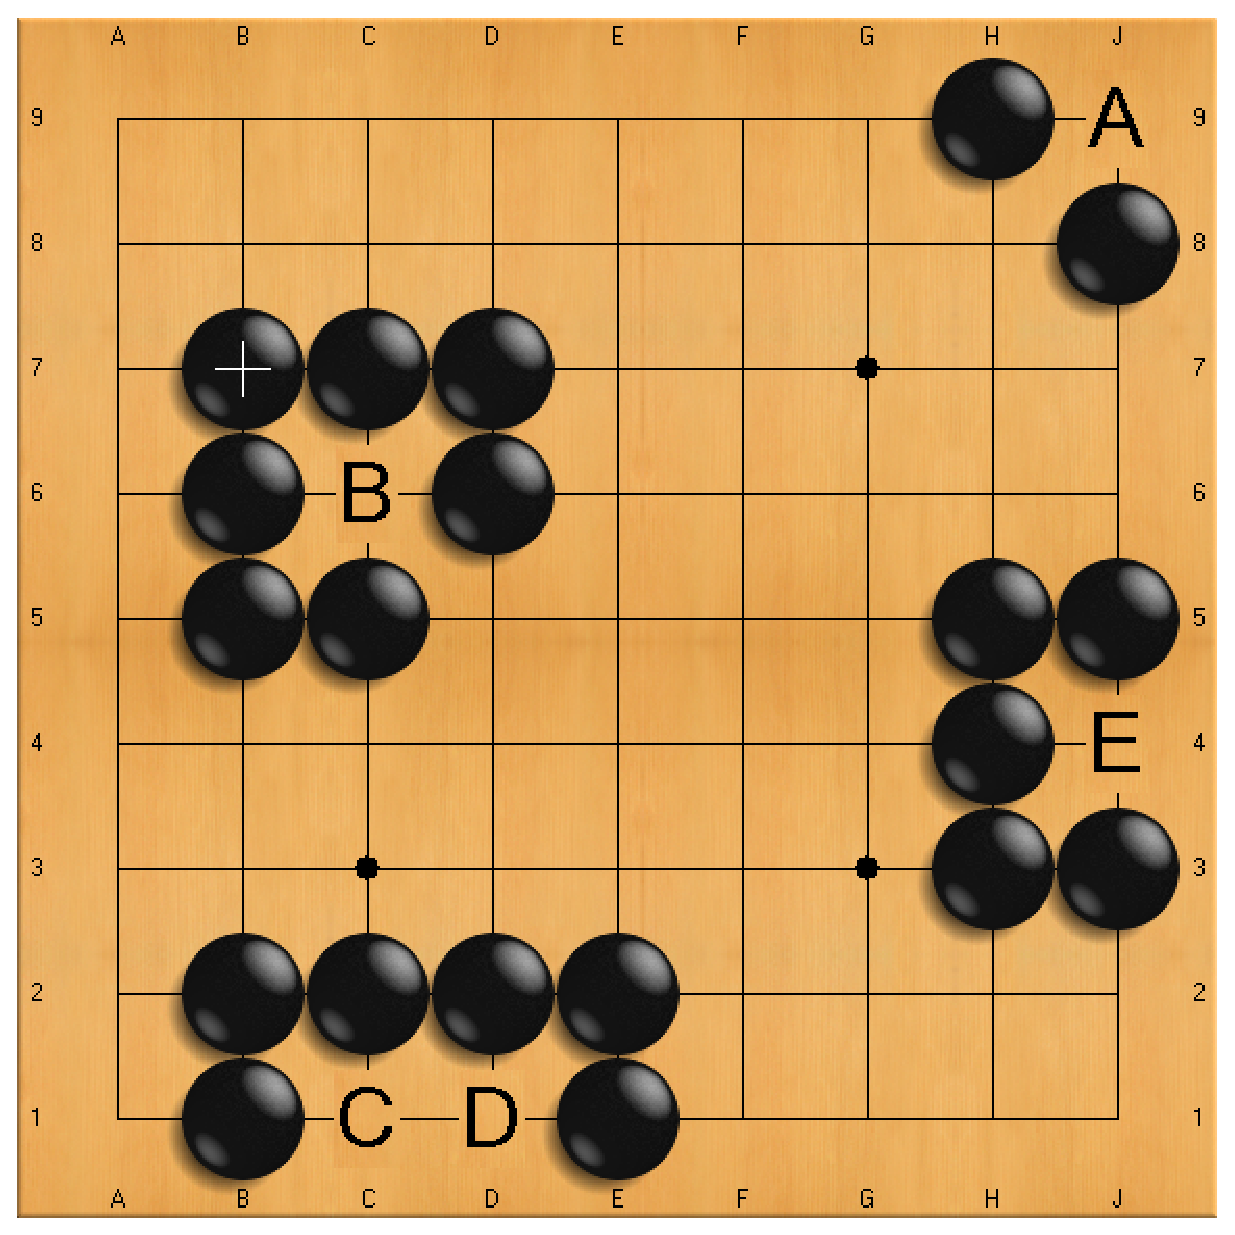
\includegraphics[scale=0.2]{contenido/cap2/imagenes/suicidio.eps}
		\caption[Situación de suicidio en el Go]{Situación de suicidio. Blancas no pueden mover en A, B o E.}
		\label{fig:go_suicidio}
	\end{minipage}
	\hspace{1cm}
	% Segunda imagen
	\begin{minipage}[t]{0.4\linewidth}
		\centering
		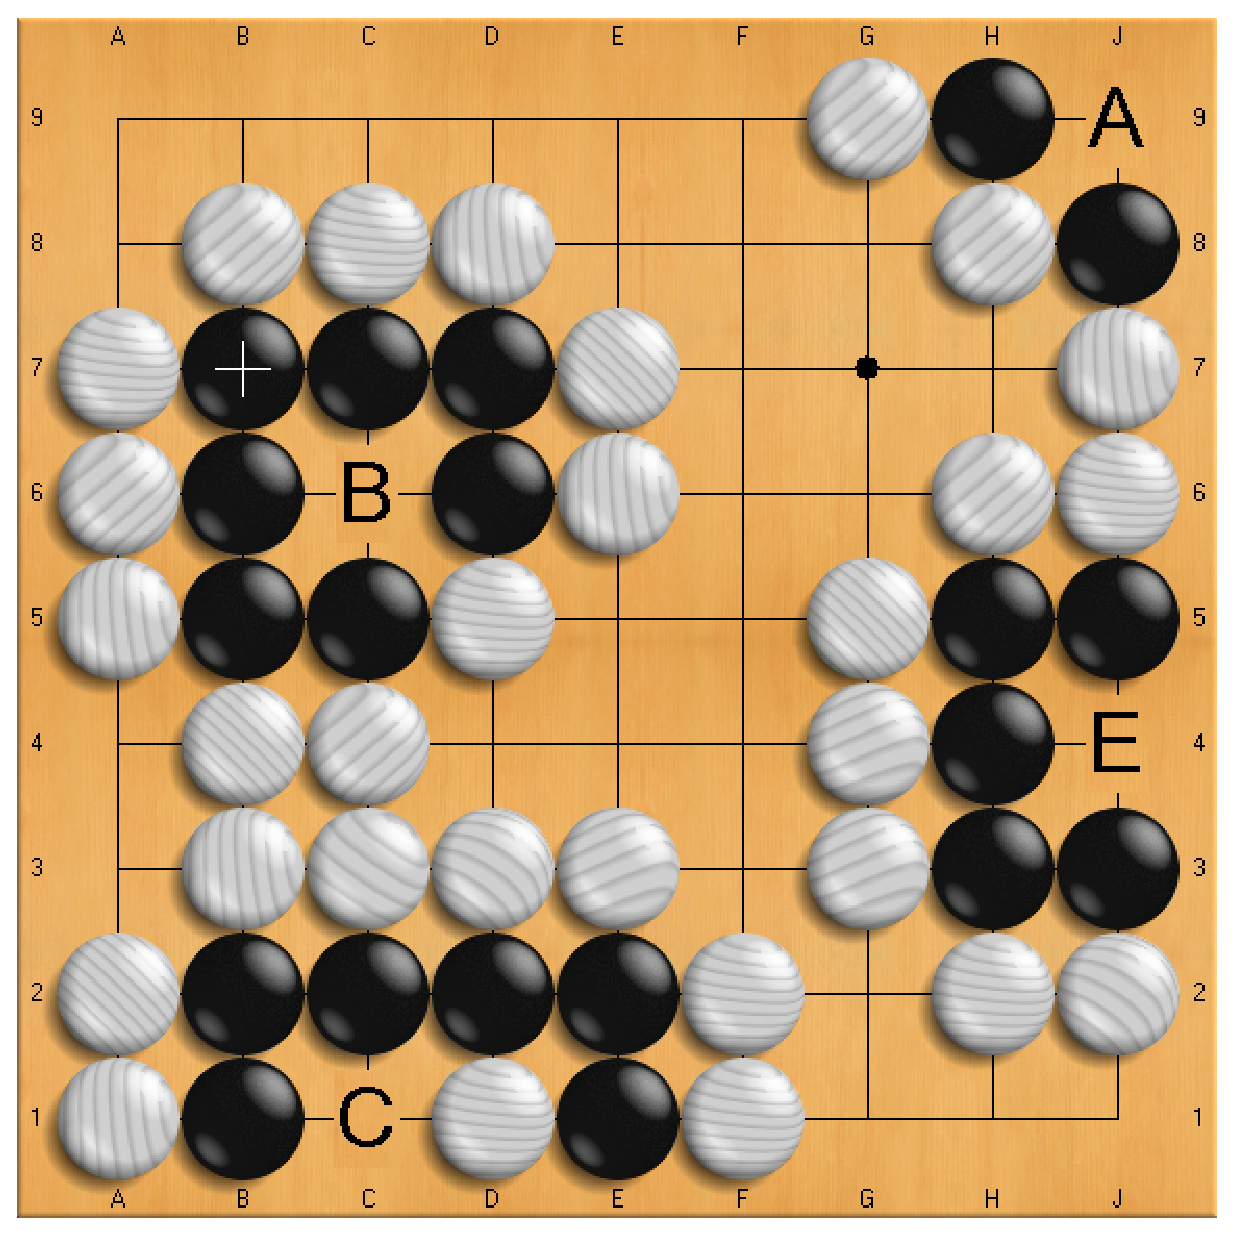
\includegraphics[scale=0.2]{contenido/cap2/imagenes/no_suicidio.eps}
		\caption[Situación de captura en el Go]{Blancas pueden mover en A, B, C o E, pues ha rodeado completamente al enemigo.}
		\label{fig:go_no_suicidio}
	\end{minipage}
\end{figure}
	\item \textbf{La regla del \textit{Ko}} \\
	La regla del \textit{Ko} evita que las posiciones de las piedras en el tablero se repitan en dos turnos diferentes.
Los tableros de la figura~\ref{fig:go_ko} reflejan esta situación.
Si un jugador captura una piedra en situación de \textit{Ko}, otro jugador no puede recapturar la misma piedra inmediatamente; ha de hacer otra jugada antes de recapturar.
Se trata de evitar una situación de infinitud.
\begin{figure}[t]
	\centering
	% Primera imagen
	\begin{minipage}[t]{0.4\linewidth}
		\centering
		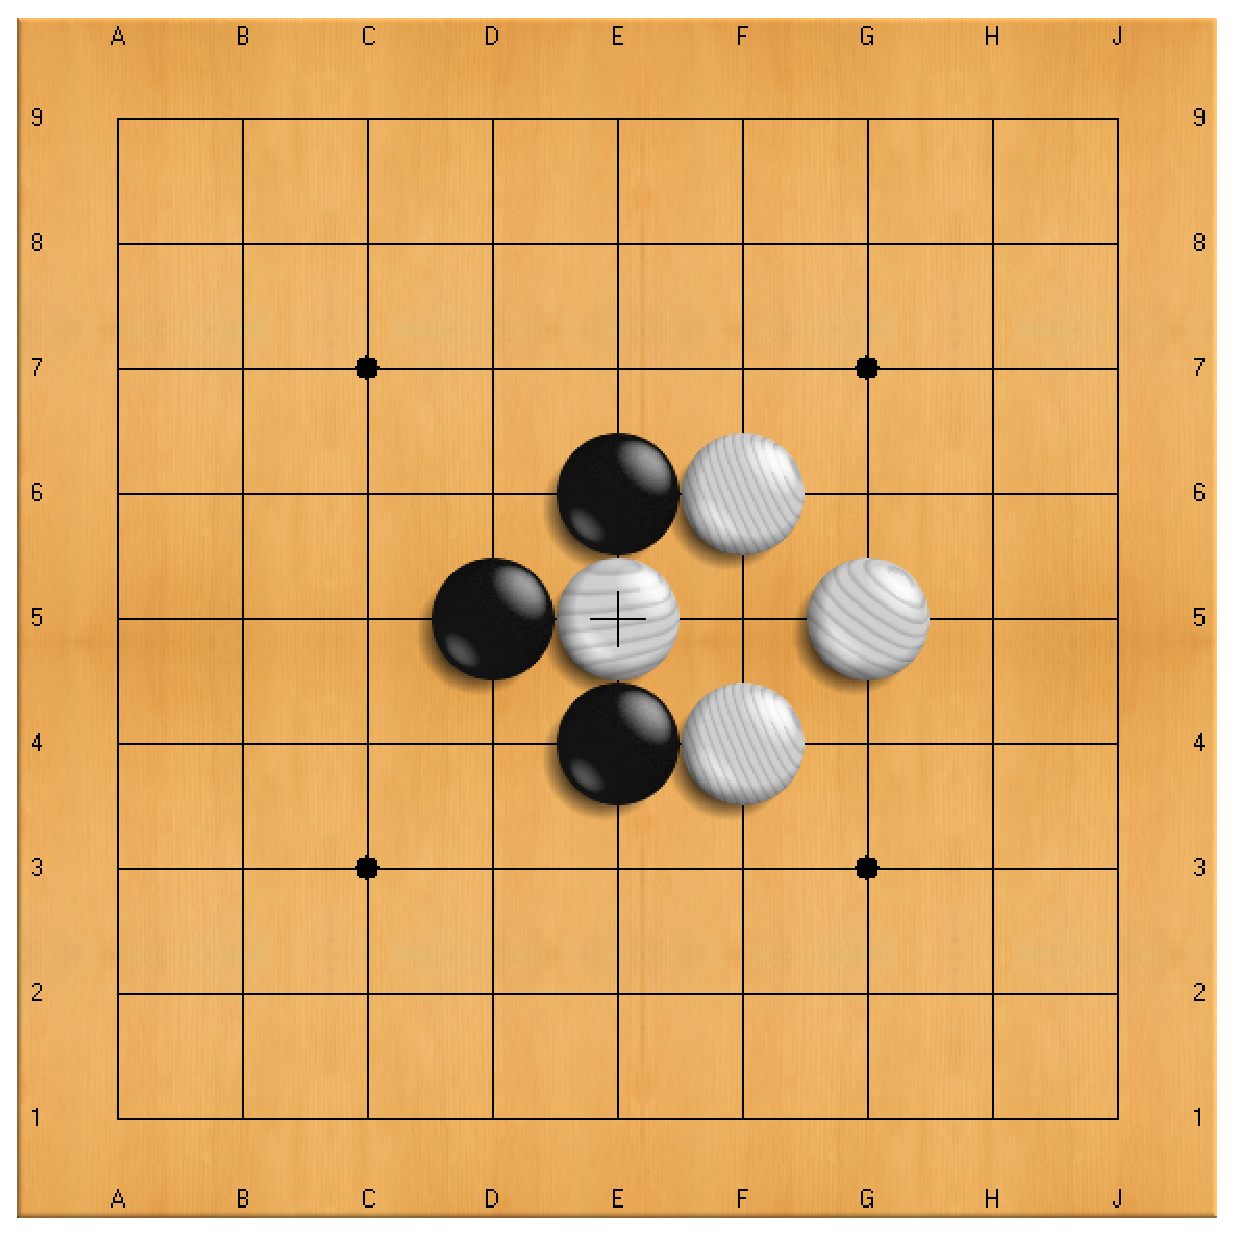
\includegraphics[scale=0.2]{contenido/cap2/imagenes/ko1.eps}
	\end{minipage}
	\hspace{1cm}
	% Segunda imagen
	\begin{minipage}[t]{0.4\linewidth}
		\centering
		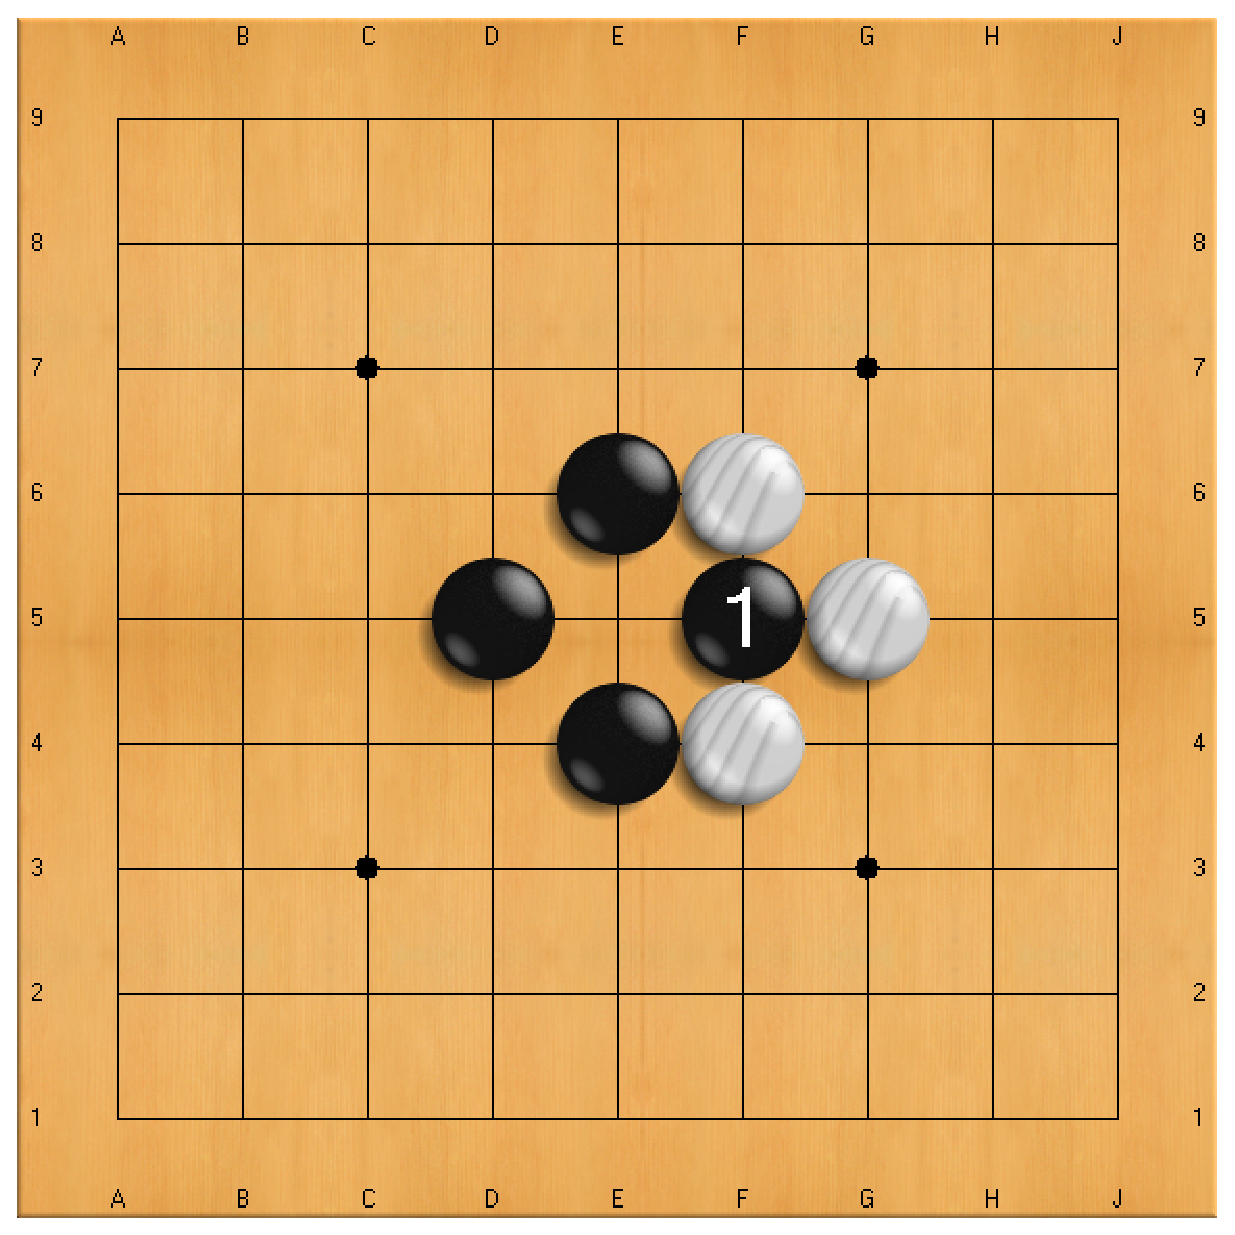
\includegraphics[scale=0.2]{contenido/cap2/imagenes/ko2.eps}
	\end{minipage}
	\caption[Situación de \textit{Ko} en el Go]{Situación de \textit{Ko}.}
	\label{fig:go_ko}
\end{figure}
\end{itemize}

Una partida de Go termina cuando ambos jugadores consideran que ya no existen territorios por disputar.
Cuando esto ocurre ambos jugadores pasan turno consecutivamente.
En una partida profesional, tal circunstancia la decide un juez.
Una partida también puede terminar si ambos jugadores han agotado sus piedras.

El \textbf{territorio} está formado por las intersecciones del tablero que se encuentren vacías.
El \textbf{territorio privado} está formado por las intersecciones que se encuentran dentro de algún cerco de uno u otro jugador.
El \textbf{territorio público} es aquel que no está cercado por ninguno de los jugadores y no influye en la puntuación final.
Hay ciertos territorios conquistados que no se encuentran protegidos del todo, pero que si el jugador contrario los atacase perdería de todas formas, luego son parte del territorio privado de quien lo tiene cercado.

El ganador de la partida es el jugador con más puntos.

\subsubsection{Puntuación}
\label{sssec:puntuacion_go}
Existen dos formas de contar los puntos de una partida: según las reglas japonesas y según las reglas chinas:

\bigskip

\begin{itemize}
	\item \textbf{Reglas japonesas}\\
	Cada jugador recibe un punto por cada intersección vacía dentro de su territorio, menos un punto por cada piedra que haya capturado el enemigo.
	\item \textbf{Reglas chinas}\\
	Cada jugador recibe un punto por cada intersección vacía dentro de su territorio, más un punto por cada piedra que tenga sobre el tablero. 
\end{itemize}
Ambos métodos producen el mismo resultado. Las reglas de puntuación japonesas son las más extendidas y son las que se usan en los torneos oficiales.

El jugador con piedras negras tiene ventaja debido a que siempre mueve primero.
Para compensar esta ventaja se suma una cantidad de puntos al jugador blanco.
A estos puntos se les denomina \textit{komi} y son determinados antes de empezar la partida.
El valor de \textit{komi} puede variar según los distintos reglamentos; suele oscilar entre 5.5 y 7.5 puntos para un tablero 19x19.
Este valor también es usado para evitar que una partida termine en empate.

\subsubsection{\textit{Handicap}}
\label{ssec:handicap_go}
En el Go existe un sistema de \textit{handicap} o ventaja para igualar una partida entre jugadores de diferente nivel.

El \textit{handicap} consiste en un número de piedras colocadas sobre el tablero antes de empezar la partida.
En ese caso el jugador de menor nivel jugará con las piedras negras y comenzará con un número determinado de piedras ya colocadas sobre el tablero.
Estas piedras se colocan sobre los puntos marcados del tablero, quedando las piedras de forma simétrica.
También existen otras variantes de \textit{handicap} libre, en el cual el jugador coloca las piedras de ventaja donde él quiera.

El número de piedras de \textit{handicap} depende de la diferencia de nivel entre los jugadores. 
Existe una clasificación oficial de niveles para los jugadores de Go \citeref{MCTS2}.









% 3. Algoritmos
\chapter{Estrategias}
\label{cap:estrategias}
Este capítulo define el concepto de \textit{agente inteligente} y profundiza en el estudio de los algoritmos que usan los agentes para juegos con adversario.
Estos algoritmos representan las estrategias usadas por los agentes para realizar los movimientos válidos en los juegos y lograr sus objetivos.

\bigskip
La siguiente sección comienza definiendo el concepto de agente de forma general.

\section{Agentes}
\label{sec:agentes}
Un \textbf{agente} o \textbf{agente inteligente} es un sistema capaz de percibir su entorno, procesar tales percepciones y actuar en su entorno de manera racional.

Un agente tiene por lo tanto un \textbf{comportamiento}: se desenvuelve en un \textbf{medio}, es capaz de percibir el medio y es capaz de actuar sobre el medio; tiene un \textbf{objetivo} y tiene \textbf{conocimiento} que le permite tomar una decisión %obtener una representación del medio y realizar un proceso de búsqueda en el mismo 
para actuar siguiendo el principio de \textbf{racionalidad}: eligiendo siempre la acción que parece acercarle más a su objetivo.

\bigskip
Antes de definir completamente nuestro agente indicando sus objetivos, conocimiento y acciones a realizar, debemos definir el medio en el que se va a desenvolver.
\section{El medio}
\label{sec:el_medio}
El \textbf{medio} o \textbf{entorno} en el que se desenvuelven nuestros agentes son los juegos con adversario, un subconjunto de los problemas de decisión Markovianos.
El entorno está definido por el espacio de estados del problema, en el caso de los juegos podemos considerar el espacio de estados como un árbol de juegos.

Un \textbf{árbol de juegos} es una representación de los estados de un juego mediante un \textit{hipergrafo}.
Un \textbf{hipergrafo} es un tipo de grafo cuyos arcos o aristas (llamadas \textbf{hiperarcos} o \textbf{hiperaristas}) pueden relacionar a cualquier cantidad de vértices, en lugar de sólo un máximo de dos.
Se caracteriza por la distinción entre 2 tipos de arcos que se denominan arcos \textit{'Y'} y arcos \textit{'O'}.
Los arcos \textit{'O'} se corresponden con aquellos definidos y utilizados en los grafos, mientras que un arco \textit{'Y'} puede apuntar a cualquier número de sucesores y representa un conjunto de posibilidades que se deben satisfacer simultáneamente.

En un árbol de juegos los nodos son los estados del juego y las aristas son los movimientos legales.
El nodo raíz del árbol es el estado inicial del juego mientras que las hojas del árbol son los estados finales del juego. 
Un camino en el árbol representa una sucesión de jugadas o movimientos en el juego.

El estado del juego está definido por la ``situación del tablero'' y el turno (el jugador al que le toca a jugar). 
Las reglas del juego limitan los movimientos legales del juego.
No todos los juegos disponen de un tablero sobre el que realizar movimientos, por ejemplo el juego de \textit{Grundy}~\citeref{grundy} o los juegos de cartas; por lo que la situación del tablero se refiere a la posición o estado de todos los elementos que intervienen en el juego (fichas, monedas, cartas, tablero, \ldots) y que permiten diferenciar un estado del juego de otro diferente.

En el capítulo~\ref{cap:juegos} se definió formalmente un juego como una clase de problemas de búsqueda con un estado inicial, una función sucesor, un test terminal y una función de utilidad.
El estado inicial y los movimientos legales para cada jugador (función sucesor) definen el árbol de juegos.
La figura~\ref{fig:arbol_juego_3enraya} muestra parcialmente el árbol de búsqueda para el juego del \textit{3 en Raya} o \textit{Tic-Tac-Toe}.
El nodo raíz es el estado inicial; el primer jugador coloca una \textit{X} en una posición vacía y a continuación se alternan los movimientos con el segundo jugador que coloca \textit{O}; finalmente se alcanzan los estados terminales en los cuales se puede asignar utilidades según las reglas del juego, en este caso +1 si gana el primer jugador (\textit{X}), -1 si gana el segundo jugador (\textit{O}) y 0 si hay empate.
\begin{figure}[h]
	\centering
	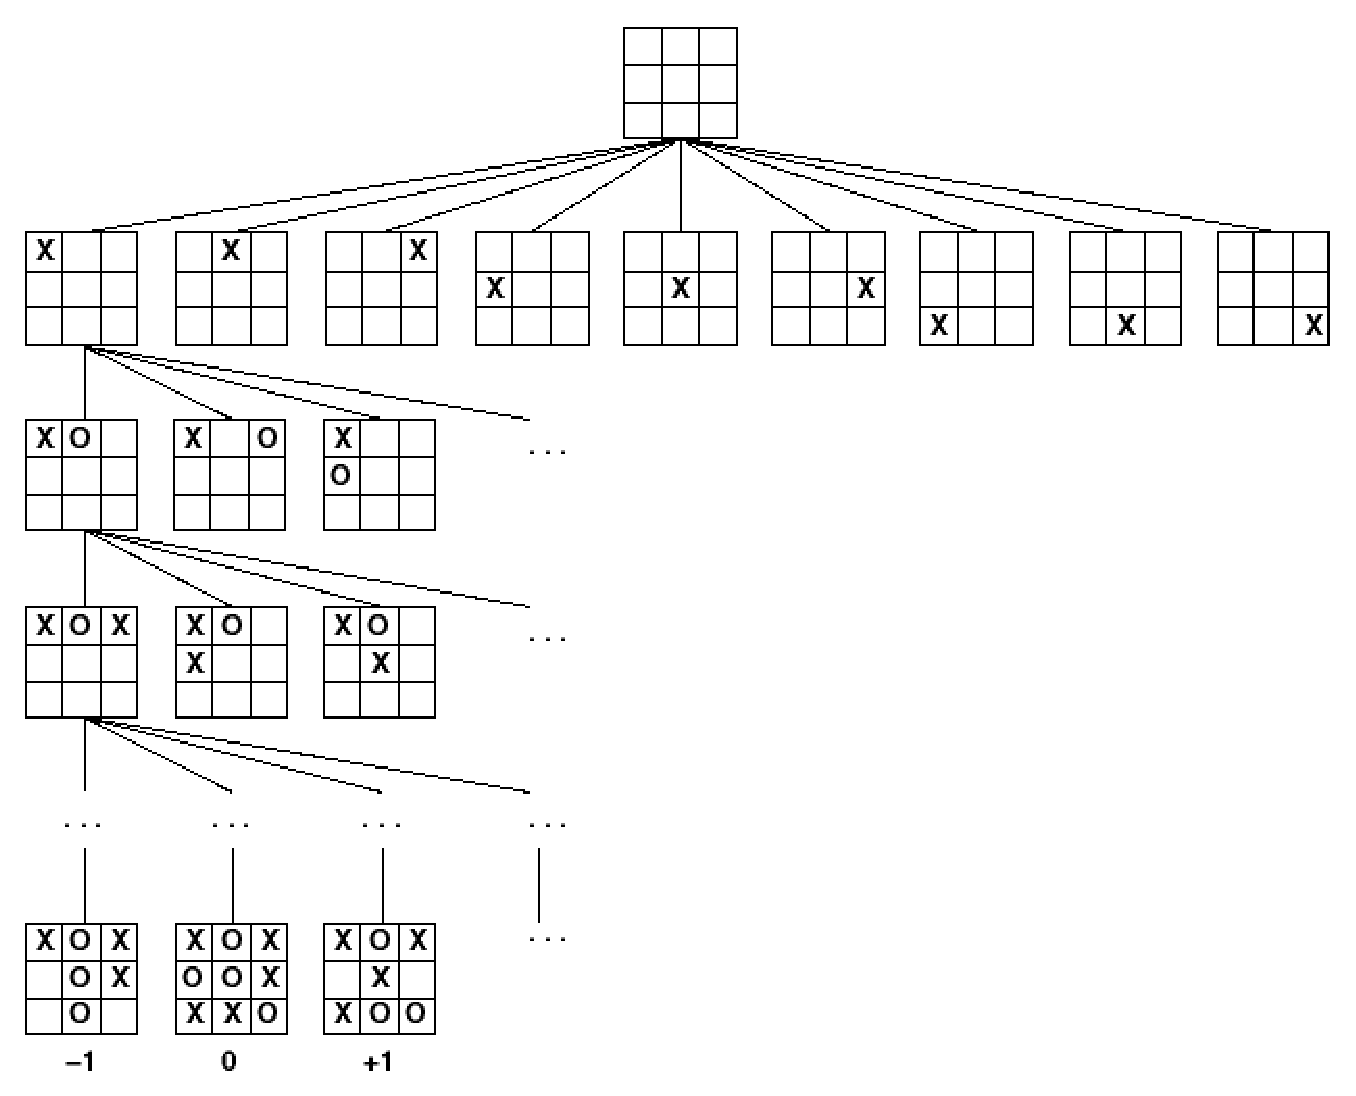
\includegraphics[scale=0.5]{contenido/cap3/imagenes/game_tree.eps}
	\caption{Árbol parcial de búsqueda para el \textit{3 en Raya}.}
	\label{fig:arbol_juego_3enraya}
\end{figure}

Los juegos a tratar son principalmente juegos bipersonales, de suma cero (si un jugador gana, el otro pierde), de información perfecta y por turnos; tal y como se definieron en el capítulo~\ref{cap:juegos} dedicado a los juegos.

\bigskip
Una vez conocido el medio en el que se desenvuelve el agente podemos completar la definición de un agente inteligente jugador de juegos.

\section{Agentes para juegos}
\label{sec:agentes_para_juegos}
En los juegos, el agente hará las veces de jugador.
Por esa razón, para referirnos a él, se utilizarán indistintamente los términos agente, agente inteligente, jugador o agente jugador.
Podemos ahora definir formalmente un agente en el contexto de los juegos.

Un \textbf{agente jugador} viene definido por los siguientes elementos:
\begin{itemize}	
	\item \textbf{El medio} \\
	El jugador se desenvuelve en el espacio de estados de un juego (representado mediante el árbol de juegos) donde otro jugador independiente (un adversario) mueve por turnos. 
	\item \textbf{Objetivos} \\
	El objetivo del agente es ganar el juego.
	\item \textbf{Percepciones} \\
	El agente es capaz de percibir el estado del juego antes de realizar cada movimiento.
	\item \textbf{Acciones} \\
	El agente es capaz de ejecutar movimientos válidos del juego.
	Pueden existir limitaciones de tiempo para realizar el siguiente movimiento.
	\item \textbf{Conocimiento} \\
	El jugador necesita una representación y una \textit{estrategia} que le permitan proponer un movimiento válido conforme a las reglas del juego.
\end{itemize}

De la sofisticación de la estrategia que use, así como de las limitaciones físicas (por ejemplo, tiempo de cálculo), dependerá la capacidad del agente para alcanzar su objetivo.

\section{Búsqueda de una estrategia ganadora}
\label{sec:busqueda_de_una_estrategia_ganadora}
Una \textbf{estrategia ganadora} es un camino (secuencia de movimientos) desde la raíz del árbol de juegos (estado inicial) hasta las hojas del árbol (estados terminales), que garantiza que el jugador gana siempre.
En la terminología introducida en la sección~\ref{sec:el_medio}, una estrategia ganadora es una solución del árbol de juegos que se corresponde con un \textbf{hipercamino solución}, es decir, un camino de arcos e hiperarcos tal que todas sus hojas son ganadoras para un jugador.

Encontrar una solución a través de una búsqueda directa desde el estado inicial hasta una posición ganadora no es factible hoy día salvo para juegos muy sencillos (como el \textit{Grundy}), ya que no es posible generar todo el árbol de búsqueda.
Incluso para un juego simple como el \textit{3 en Raya} es complejo dibujar el árbol de juegos completo.
La tabla~\ref{tab:complejidad_juegos} presentada en el capítulo~\ref{cap:juegos} muestra este hecho.
% poner tabla de juegos y complejidad en relacion al factor de ramificacion.

Por lo tanto no se puede conocer de antemano una estrategia ganadora para un jugador; y en la mayoría de los casos hay que conformarse con obtener una buena jugada a partir de una configuración dada.
Esto obliga al agente a tomar algún tipo de decisión para realizar los movimientos del juego.

\bigskip
En la siguiente sección se estudiarán las diferentes estrategias y algoritmos propuestos que usarán los agentes.

\section{Estrategias}
\label{sec:estrategias}
A continuación se estudian los algoritmos y estrategias desarrollados.
Todas las estrategias han sido incluidas en la aplicación interactiva para poder usarlas: jugar con ellas, analizarlas y compararlas.
Los algoritmos estudiados son versiones generales de los mismos con el objetivo de que sean sencillos de entender y resulten útiles para la docencia.
Versiones más sofisticadas de los algoritmos propuestos pueden ser desarrolladas e incluidas en la aplicación como se explica en el apéndice~\ref{cap:desarrollo_juegos_estrategias_heuristicos}.

%\bigskip
% PONER ESTO EN LA INTRODUCCION.
%Implementarán versiones generales de estas estrategias de forma que resulten
%sencillas de entender de cara a la docencia. Estas van desde el caso más básico
%como la estrategia aleatoria hasta algoritmos más complejos como una estrategia
%con aprendizaje u otra con redes neuronales, pasando por los clásicos
%algoritmos de evaluación minimax y poda alfa-beta, entre otros.
%Además de las estrategias que se detallan a continuación, para cada juego
%se implementará un jugador que pida el movimiento al usuario. De esta
%manera un jugador humano podrá jugar contra cualquier estrategia o incluso
%contra otro jugador humano.

\subsection{Aleatoria}
\label{ssec:aleatoria}
La estrategia más sencilla es un jugador que realice movimientos aleatorios.
Este jugador es totalmente independiente del juego.

Un agente con una estrategia aleatoria obtiene todos los posibles estados sucesores a partir del estado actual del juego y elige uno de ellos de forma aleatoria.
Esta forma de proceder es ineficiente para juegos con un factor de ramificación elevado;
pero evita que el agente deba conocer cómo se generan los estados para cada juego, ya que los estados sucesores son generados por el propio estado actual del juego, tal y como se definió en~\ref{sec:juegos_problemas_busqueda_adversario}.
Esto hace que el agente pueda jugar a cualquier tipo de juego.

Una estrategia aleatoria tampoco ayuda al agente a lograr su objetivo (ganar) de una forma directa;
pero será de gran utilidad como base para comparar el rendimiento del resto de estrategias, además de servir como estrategia oponente en los entrenamientos de los agentes que lo requieran. 

\subsection{Evaluador heurístico}
\label{ssec:evaluador_heuristico}
Un agente evaluador heurístico es capaz de evaluar heurísticamente si una situación dada le es favorable o no.

El agente emplea la siguiente estrategia de juego: \emph{dada una situación, considera todos los movimientos inmediatos, los evalúa heurísticamente y escoge el mejor.}

Esta estrategia, al contrario que la estrategia aleatoria, no es totalmente independiente del juego, pues necesita de una función de evaluación heurística que depende del tipo de juego.

Cualquier jugador que necesite de una función de evaluación heurística puede considerarse como una especialización de este agente.
El capítulo~\ref{cap:heuristicos} está dedicado a los evaluadores heurísticos que pueden usar los agentes.

%\bigskip
%La siguiente sección estudia la estrategia minimax y los agentes desarrollados que emplean dicha estrategia.

\subsection{Minimax}
\label{ssec:minimax}
Antes de presentar los agentes que emplean la estrategia minimax, se detallará el algoritmo minimax de forma general, así como la variante implementada: negamax.

\bigskip
El \textbf{algoritmo minimax} proporciona una estrategia óptima, aunque en la práctica no es factible calcularla para juegos complejos.
Una \textbf{estrategia óptima}, en un problema de búsqueda normal, es una secuencia de movimientos que conducen a un estado objetivo (un estado terminal que es ganador).
Sin embargo, en problemas de búsquedas con adversario, el otro jugador también participa y su objetivo es el mismo y opuesto al del primer jugador, por lo que deberá usar una estrategia contingente.
Podemos decir que una estrategia óptima conduce a resultados al menos tan buenos como cualquier otra estrategia cuando uno juega con un oponente infalible.

La estrategia minimax consiste en realizar un análisis desde la posición actual y generar una serie de jugadas posibles por parte de ambos jugadores.
Una vez alcanzado el nivel de profundidad deseado en el árbol de juegos se utiliza una función de evaluación que asigna valores numéricos a las posiciones finales, lo que permite, además de elegir la mejor posición, transmitir esta información hasta la posición actual que corresponde a la raíz del árbol generado. 
Minimax sólo tiene en cuenta una visión local del árbol de búsqueda.

Llamaremos al primer jugador \textit{MAX} y al segundo jugador \textit{MIN}; y etiquetaremos los niveles del árbol con \textit{MAX} y \textit{MIN} según le toque jugar a \textit{MAX} o \textit{MIN} respectivamente.

Considerando un árbol de juegos, la estrategia óptima puede determinarse examinando el valor minimax de cada nodo, que llamamos \textit{VALOR\_MINIMAX(n)}.
El valor minimax de un nodo es la utilidad (para \textit{MAX}) de estar en el estado correspondiente, asumiendo que ambos jugadores juegan óptimamente desde allí hasta el final del juego.
El valor minimax de un estado terminal es su utilidad.
Considerando una opción, \textit{MAX} prefiere mover a un estado de valor máximo, mientras que \textit{MIN} prefiere un estado de valor mínimo. 
Se define entonces el \textit{VALOR\_MINIMAX(n)} de un nodo como:
{\footnotesize
\begin{equation}
VALOR\_MINIMAX(n) = 
\left\{\begin{array}{ll}
UTILIDAD(n) & \textnormal{si \textit{n} es un estado terminal}\\
\max_{s\in Sucesores(n)} VALOR\_MINIMAX(s) & \textnormal{si \textit{n} es un estado \textit{MAX}}\\
\min_{s\in Sucesores(n)} VALOR\_MINIMAX(s) & \textnormal{si \textit{n} es un estado \textit{MIN}}\\
\end{array}\right. \label{eq:minimax}
\end{equation}
}

La figura~\ref{fig:minimax} muestra el funcionamiento del algoritmo minimax para un árbol de juegos.
Los nodos $\Box$ son <<nodos \textit{MAX}>>, en los que le toca mover a \textit{MAX}, y los nodos $\bigcirc$ son <<nodos \textit{MIN}>>.
Los nodos terminales muestran los valores de utilidad para \textit{MAX}; los otros nodos son etiquetados por sus valores minimax.

\begin{figure}[h]
	\centering
	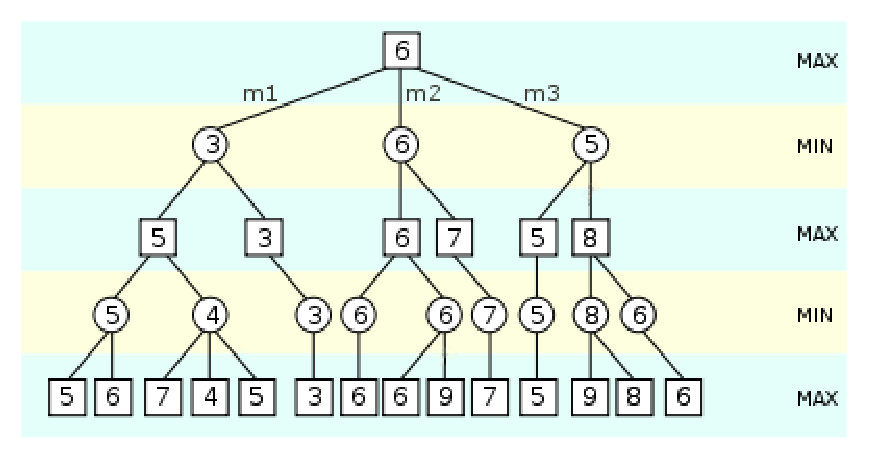
\includegraphics[scale=0.8]{contenido/cap3/imagenes/minimax.eps}
	\caption{Minimax aplicado a un árbol de juegos.}
	\label{fig:minimax}
\end{figure}

Se realiza una exploración hacia delante, generando primero el árbol completo a una determinada profundidad (cuatro en este caso), a continuación se evalúan las hojas con la función de utilidad y los valores se propagan hacia arriba de la siguiente forma:
\begin{itemize}
\renewcommand{\labelitemi}{-}
	\item Un nodo \textit{MAX} toma como valor el máximo de sus hijos.
	\item Un nodo \textit{MIN} toma como valor el mínimo de sus hijos.
\end{itemize}
Finalmente, el movimiento de \textit{MAX} es el mejor valorado de sus hijos inmediatos, que en el caso de la figura~\ref{fig:minimax} se trata del movimiento \textit{m2}.

Esta forma de proceder es más fiable que evaluar solamente los hijos inmediatos, como hacía el agente evaluador heurístico presentado en la sección~\ref{ssec:evaluador_heuristico}.
La función de utilidad que usa minimax para asignar los valores a los nodos evaluados es una función de evaluación heurística, puesto que en la mayoría de los casos los estados a evaluar no serán terminales.
Esta función se define en el capítulo~\ref{cap:heuristicos} dedicado a los evaluadores heurísticos.

El algoritmo minimax realiza una exploración primero en profundidad.
Para una búsqueda en un árbol a profundidad \textit{p} y un factor de ramificación \textit{b}, minimax evaluará $b^p$ nodos hojas.
La complejidad en tiempo del algoritmo minimax es $O(b^p)$; y la complejidad en espacio es $O(bp)$ si se generan todos los sucesores a la vez, o $O(p)$ si se generan uno por uno.
Para juegos reales, los costes de tiempo son impracticables, pero este algoritmo sirve como base para el análisis matemático de juegos y para otros algoritmos más prácticos.

Existen numerosas mejoras del algoritmo minimax original; algunas de ellas consisten en realizar:
\begin{itemize}
	\item una búsqueda en profundidad con retroceso (\textit{backtrack}),
	\item una búsqueda con profundización progresiva (\textit{algoritmos anytime}),
	\item explorar sólo la parte imprescindible del árbol (\textit{poda alfa-beta}), o
	\item almacenar información sobre los estados visitados anteriormente  y usarla cuando nos encontremos esos estados por otro camino del árbol (\textit{tablas de transposiciones}).
\end{itemize}
A continuación se detallan cada una de estas mejoras que se han implementado e incorporado a la aplicación; presentando primero la variante implementada del algoritmo minimax: negamax.

\subsubsection{Negamax}
\label{sssec:negamax}
En lugar del algoritmo minimax propiamente dicho se ha implementado una variante equivalente conocida como \textbf{negamax}.
En esta variante, cada nodo del árbol de juegos toma siempre el valor máximo de sus hijos, independientemente de que sea un nodo \textit{MAX} o \textit{MIN}.
Adicionalmente, los valores de los nodos \textit{MAX} se cambian de signo.
De este modo, es equivalente para un nodo \textit{MIN} tomar el máximo de las evaluaciones cambiadas de signo, que tomar el mínimo de las evaluaciones sin alterar.
El origen de negamax se basa en la igualdad matemática:
\begin{displaymath}
\max{(x, y)} = - \min{(-x, -y)}
\end{displaymath}

Negamax no supone una mejora directa de minimax, sino que se trata más bien del algoritmo minimax comprimido que evita tener que definir dos funciones distintas para \textit{MAX} y \textit{MIN}.
Además, se sigue teniendo el mismo problema de la complejidad que supone explorar el árbol de juegos al completo.
Para evitar esto se ha modificado la versión original de negamax dando lugar a dos agentes que emplean dos estrategias diferentes: una con profundidad máxima de búsqueda y otra con un límite de tiempo.

\subsubsection{Minimax con profundidad máxima de búsqueda}
\label{sssec:profundidad_maxima_busqueda}
El primer agente emplea una estrategia con la variante negamax y un parámetro adicional que indica la profundidad máxima de búsqueda en el árbol de juegos a partir de la posición actual.

La estrategia comienza en la posición actual y realiza una búsqueda en profundidad con retroceso (\textit{backtrack}) hasta la profundidad de búsqueda indicada.
Los sucesores son generados aleatoriamente de uno en uno y en cada paso el algoritmo se queda con el mejor movimiento en función del valor minimax devuelto.

% PONER ESTO EN DISEÑO.
%El algoritmo minimax y su variante negamax es recursivo por naturaleza y así ha sido implementado; aunque esto pueda parecer un inconveniente en cuanto a la eficiencia, el algoritmo resultante es muy fácil de entender y esto era uno de los objetivos de este proyecto, por encima de la eficiencia obtenida en los algoritmos.
%Además, una versión iterativa de los mismos no siempre supone una mejora en la eficiencia, debido al gran aumento en complejidad que supone desarrollar y gestionar una estructura temporal (por ejemplo una pila) para almacenar la información de la recursividad.

Este agente puede evaluar posiciones a una profundidad dada.
Sin embargo, incrementos lineales de profundidad pueden originar búsquedas que requieran un tiempo exponencialmente mayor.
Del mismo modo, aún sin variar la profundidad, el tiempo necesario para la búsqueda puede ser muy variable.
Normalmente el número de posibilidades al comienzo de un juego es mucho mayor que a medida que se desarrolla la partida, por lo que examinar los movimientos iniciales puede llevar un tiempo mayor.

La limitación del tiempo de cómputo puede superarse empleando un algoritmo que en cualquier momento pueda dar una solución, pero que proporcione soluciones mejores cuanto mayor sea el tiempo disponible.
Los algoritmos que presentan esta propiedad se conocen como algoritmos \textit{anytime}.
El siguiente agente, que también emplea una estrategia minimax, dispone de un límite de tiempo para realizar la búsqueda, en lugar de un límite en la profundidad máxima de búsqueda.

\subsubsection{Minimax con límite de tiempo}
\label{sssec:limite_tiempo}
El segundo agente también emplea negamax pero dispone de un tiempo limitado para realizar la búsqueda del mejor movimiento en el árbol de juegos.

Se trata de un algoritmo \textit{anytime}.
Un \textbf{algoritmo \textit{anytime}} devuelve una solución cuya calidad depende del tiempo de cómputo disponible.
El algoritmo encontrará mejores soluciones a medida que aumenta el tiempo disponible para realizar la búsqueda.

La estrategia realiza una búsqueda con retroceso y profundización progresiva (\textit{Backtrack with Iterative Deepening}.
La búsqueda dispone de una cota (profundidad máxima de búsqueda) que se incrementa automáticamente en cada iteración.
El algoritmo guarda siempre la mejor jugada inmediata para la última exploración realizada con objeto de devolverla cuando el tiempo se acabe.
En cada iteración el algoritmo comprueba el tiempo restante, terminando la búsqueda cuando este se agota.

Puede darse el caso de que el límite de tiempo sea tan pequeño que la estrategia no tenga tiempo de devolver un movimiento, en ese caso el agente acabará realizando un movimiento aleatorio.
Además, para asegurarse de devolver el mejor movimiento, la estrategia debe evaluar todos los nodos del nivel del árbol que corresponde a la cota de la iteración actual.
Si en la iteración actual no ha tenido tiempo de evaluarlos todos, devolverá el mejor movimiento obtenido en la iteración anterior.

Por simplicidad, la unidad de tiempo escogida ha sido el segundo, pues para la mayoría de juegos no tiene sentido dejar menos tiempo de cómputo al agente debido a la complejidad de los propios juegos.
Esto implica que el tiempo mínimo permitido sea de un segundo.


\bigskip
Una vez vista la estrategia básica minimax y su variante negamax, dedicaremos la siguiente sección a estudiar otra mejora de minimax: la poda alfa-beta.

\subsection{Poda alfa-beta}
\label{ssec:poda_alfa_beta}
Esta sección estudia la técnica de la poda alfa-beta como una mejora del algoritmo minimax.
También define los agentes que emplearán esta estrategia, que al igual que ocurría con minimax serán dos: uno con límite de profundidad en la búsqueda y otro con un límite en el tiempo de cómputo.

\bigskip
La \textbf{poda alfa-beta} calcula el mismo movimiento que devolvería minimax sin necesidad de examinar todos los nodos en el árbol de juegos, es decir, poda las ramas del árbol que no influyen en la decisión final.

Esta estrategia dispone de dos parámetros ($\alpha$ y $\beta$) que describen los límites sobre los valores que se propagan hacia arriba en el árbol:
\begin{itemize}
	\item $\alpha$ es el valor de la mejor opción (es decir, el valor más alto) que se ha encontrado hasta ahora en cualquiera de los estados elegidos para \textit{MAX}. 
	\item $\beta$ es el valor de la mejor opción (es decir, el valor más bajo) que se ha encontrado hasta ahora en cualquiera de los estados elegidos para \textit{MIN}.
\end{itemize}
La poda alfa-beta realiza una búsqueda primero en profundidad, con retroceso y de izquierda a derecha.
Para cada nodo se considera un intervalo de posibles valores [$\alpha$, $\beta$].
La búsqueda actualiza estos valores según recorre el árbol: actualiza el valor $\alpha$ (en los nodos \textit{MAX}) y el valor $\beta$ (en los nodos \textit{MIN}).
Cuando encuentra un nodo con un valor peor que su antecesor, la búsqueda se detiene y esa rama del árbol no se examina.
Así, se puede podar:
\begin{itemize}
\renewcommand{\labelitemi}{-}
	\item Debajo de un nodo \textit{MIN} cuando un nodo \textit{MAX} antecesor suyo tenga un valor $\alpha \geq \beta$; lo que se conoce como \textbf{corte $\alpha$}.
	\item Debajo de un nodo \textit{MAX} cuando un nodo \textit{MIN} antecesor suyo tenga un valor $\beta \leq \alpha$; lo que se conoce como \textbf{corte $\beta$}.
\end{itemize}

La figura~\ref{fig:alfabeta} muestra el funcionamiento de la poda alfa-beta para el mismo árbol de juegos de la figura~\ref{fig:minimax}.
Los nodos \textit{MAX} muestran el valor final de $\alpha$ mientras que los nodos \textit{MIN} muestran el valor final de $\beta$.
El valor minimax devuelto por la poda alfa-beta para el nodo raíz es el mismo que el valor devuelto por el algoritmo minimax y en este caso, el movimiento es también el mismo (\textit{m2}).

\begin{figure}[h]
	\centering
	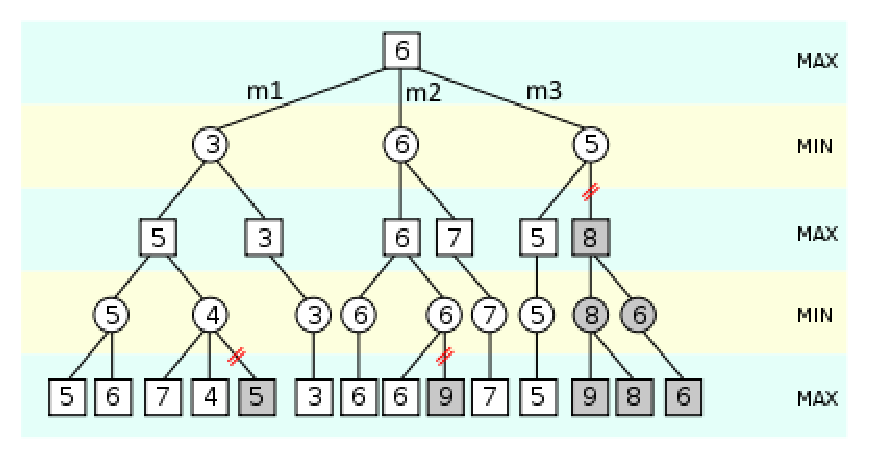
\includegraphics[scale=0.8]{contenido/cap3/imagenes/podaalfabeta.eps}
	\caption{Poda alfa-beta aplicada a un árbol de juegos.}
	\label{fig:alfabeta}
\end{figure}

En los agentes desarrollados esto no siempre es así y puede ocurrir que el mejor movimiento devuelto por minimax sea distinto del mejor movimiento devuelto por alfa-beta (pero ambos tendrán el mismo valor de evaluación); esto se debe a que los sucesores son generados en orden aleatorio y además, en el caso de que más de un estado tenga la misma evaluación, minimax cogerá el último sucesor que evalúe mientras que alfa-beta puede podar esa rama si encontró otro nodo con la misma evaluación.

La eficacia de la poda alfa-beta depende mucho del orden en el que se examinan los sucesores.
Una posible mejora del algoritmo sería examinar primero los sucesores que probablemente sean mejores.
Para una búsqueda en un árbol a profundidad \textit{p} y un factor de ramificación \textit{b}, en el mejor caso (los nodos están ordenados de mejor a peor), alfa-beta tiene que examinar $O(b^{p/2})$ nodos para escoger el mejor movimiento, en vez de $O(b^p)$ para minimax.% lo que reduce a la mitad el tiempo necesario.
En los algoritmos desarrollados donde los sucesores se examinan en orden aleatorio, el número total de nodos examinados es de $O(b^{3p/4})$.
Por último, en el peor de los casos, donde no se realiza ninguna poda, la complejidad es la misma que en minimax: $O(b^p)$.

\bigskip
A continuación se presentan los agentes que emplean la técnica de la poda alfa-beta, al igual que ocurría con minimax se trata de dos agentes con características diferentes: uno con un límite en la profundidad de búsqueda y otro con un tiempo limitado de búsqueda.

\subsubsection{Alfa-beta con profundidad máxima de búsqueda}
\label{sssec:profundidad_maxima_busqueda_alfabeta}
Este agente emplea el algoritmo negamax con poda alfa-beta incluida para realizar una búsqueda en el árbol de juegos a una profundidad máxima indicada a partir de la posición actual.

La lógica del agente es la misma que la explicada para el agente minimax con profundidad máxima de búsqueda (apartado~\ref{sssec:profundidad_maxima_busqueda}), con el incentivo de que incorpora la poda alfa-beta.

\subsubsection{Alfa-beta con límite de tiempo}
\label{sssec:limite_tiempo_alfabeta}
El segundo agente también emplea el algoritmo negamax con poda alfa-beta y dispone de un tiempo limitado para realizar la búsqueda del mejor movimiento en el árbol de juegos.

El agente tiene las mismas características que el agente minimax con límite de tiempo (descrito en el apartado~\ref{sssec:limite_tiempo}), pero incluyendo además las ventajas de la poda alfa-beta.


\bigskip
Otra mejora con respecto al algoritmo minimax original y de alfa-beta es la posibilidad de incorporar una tabla de transposición a la búsqueda.
En la siguiente sección se estudian las tablas de transposición.

\subsection{Tablas de transposición}
\label{ssec:tablas_transposicion}
Esta sección desarrolla los conceptos de \textit{transposición} y \textit{tabla de transposición} para las búsquedas en árboles de juegos.
Se presentan también los agentes que emplean esta técnica.

\bigskip
Una \textbf{transposición} es una permutación diferente de una secuencia de movimientos que termina en la misma posición.
En el árbol de juegos se trata de un estado que puede ser alcanzado por más de un camino distinto.

Los estados repetidos en el árbol de búsqueda pueden causar un aumento exponencial del coste de la búsqueda.
Es por ello que merece la pena almacenar la evaluación de ese estado en una tabla la primera vez que se encuentre, de modo que no tenga que volver a calcularse la próxima vez que se visite.
A esta tabla se le conoce como tabla de transposición.

Una \textbf{tabla de transposición} o \textbf{tabla de transposiciones} es una base de datos donde se almacenan los resultados de búsquedas previamente realizadas.
Normalmente se implementa mediante una tabla \textit{hash} de gran capacidad y se almacenan los estados previamente evaluados, hasta qué nivel se les realizó la búsqueda y qué acción se determinó para estos; aunque pueden almacenar más información si es necesario.

Se trata de una forma de reducir el espacio de búsqueda.
Cuando aparece una transposición, se busca en la tabla qué se determinó la última vez; evitando repetir de nuevo toda la búsqueda y pudiendo invertir ese ahorro de tiempo en aumentar la profundidad de búsqueda.

La utilización de una tabla de transposición puede tener un efecto espectacular en situaciones donde hay muchas posibles transposiciones como en la etapa final de los juegos (por ejemplo en el Ajedrez).
Por otra parte, el único problema de las tablas de transposiciones es su consumo en memoria.
Para que sean realmente útiles deben contener muchas posiciones y si se evalúan un millón de nodos por segundo no es práctico almacenar todos ellos en la tabla de transposición.

\bigskip
Los agentes que emplean las tablas de transposición son los mismos que se han presentado anteriormente para minimax y alfa-beta pero incorporando esta nueva característica, lo que da lugar a cuatro nuevos agentes que se presentan brevemente en los siguientes apartados.

\subsubsection{Minimax con profundidad máxima de búsqueda y tabla de transposición}
\label{sssec:minimax_profmax_tablatransposicion}
Se trata de un agente que realiza una búsqueda en el árbol de juegos mediante el algoritmo minimax, dispone de un límite en la profundidad máxima de búsqueda a partir del estado actual y cuenta con una tabla de transposición para almacenar los estados evaluados y usar la información guardada en caso de encontrar una transposición.

Para más información sobre este agente se puede consultar el agente minimax con profundidad máxima de búsqueda en la sección~\ref{sssec:profundidad_maxima_busqueda}.

\subsubsection{Minimax con límite de tiempo y tabla de transposición}
\label{sssec:minimax_limiteTiempo_tablatransposicion}
Este agente realiza una búsqueda en el árbol de juegos empleando el algoritmo minimax, dispone de un límite de tiempo para devolver el mejor movimiento y cuenta con una tabla de transposición.

La sección~\ref{sssec:limite_tiempo} contiene información sobre el agente minimax con límite de tiempo.

\subsubsection{Alfa-beta con profundidad máxima de búsqueda y tabla de transposición}
\label{sssec:alfabeta_profmax_tablatransposicion}
Este agente emplea el algoritmo minimax con poda alfa-beta incluida para realizar la búsqueda en el árbol de juegos; tiene una profundidad máxima de búsqueda y se ayuda de una tabla de transposición para evitar evaluar los estados repetidos.

En la sección~\ref{sssec:profundidad_maxima_busqueda_alfabeta} se detalla el agente alfa-beta con profundidad máxima de búsqueda, que cuenta con las mismas características que este, salvo obviamente, la tabla de transposición.

\subsubsection{Alfa-Beta con límite de tiempo y tabla de transposición}
\label{sssec:alfabeta_limiteTiempo_tablatransposicion}
El último agente también usa el algoritmo minimax con poda alfa-beta; tiene un límite de tiempo para realizar la búsqueda en el árbol y también cuenta con una tabla de transposición.

El agente alfa-beta con límite de tiempo puede consultarse en la sección~\ref{sssec:limite_tiempo_alfabeta}.

\bigskip
A continuación se describen los agentes que no necesitan de un evaluador heurístico para determinar el mejor movimiento, estos son los agentes que usan el método de Monte-Carlo y Monte-Carlo Tree Search.
Ambas estrategias son totalmente independientes del tipo de juego, ya que no necesitan de una función de evaluación heurística.

\subsection{Monte-Carlo}
\label{ssec:montecarlo}
Esta sección explica el método de Monte-Carlo aplicado a los problemas de búsqueda en árboles de juegos.
Se estudia una versión básica del mismo y se presentan los agentes que lo usan.

El \textbf{método de Monte-Carlo} consiste en realizar un número de simulaciones a partir del estado actual para decidir el próximo movimiento.

Una \textbf{simulación} es una partida al azar completa del juego desde la posición actual; es decir, partiendo del estado actual en el árbol de juegos, se realizan movimientos aleatorios hasta llegar a un estado terminal, donde se asigna el valor de utilidad (+1, -1 ó 0 si es el estado es ganador, perdedor o empate para el jugador).
Este valor es usado como la recompensa esperada que se puede obtener a partir del estado sucesor elegido.
Para estimar el valor final de un estado se toman estadísticas haciendo un promedio de las recompensas obtenidas en las simulaciones.

El método genera una lista de posibles movimientos (sucesores del estado actual) y para cada movimiento realiza miles de simulaciones (partidas al azar), obteniendo el valor de recompensa.
El movimiento con un valor de recompensa mayor es el elegido como mejor movimiento, es decir, aquel que conduce a la mejor serie de partidas al azar para el jugador actual.

La ventaja de esta técnica es que requiere poco conocimiento del entorno, pero se incrementan los requisitos computacionales (procesador y memoria).
Para que el método sea efectivo se deben realizar muchísimas simulaciones, ya que los movimientos de las simulaciones se generan al azar y es posible que una buena jugada sea evaluada erróneamente como una mala jugada.

A priori es difícil establecer de antemano un número determinado de simulaciones, por lo que se suele dejar un tiempo máximo para realizar las simulaciones.

\bigskip
Los siguientes apartados presentan dos agentes que usan el método de Monte-Carlo: uno con un número determinado de simulaciones y otro con un límite de tiempo para realizar las simulaciones.

\subsubsection{Monte-Carlo con número de simulaciones fijas}
\label{sssec:montecarlo_simulaciones}
El jugador Monte-Carlo más simple es aquel que tiene un número de simulaciones determinado.

Partiendo del estado actual juega el número de partidas indicadas para evaluar el mejor movimiento.
Para cada sucesor del estado actual se realiza un número diferente de simulaciones, pues estos también son elegidos aleatoriamente.
El número de simulaciones debe ser suficientemente grande para asegurarse de que se realizan aproximadamente el mismo número de simulaciones para cada posible movimiento.
Si \textit{N} es el número total de simulaciones a realizar y \textit{p} es el número de sucesores del estado actual, se espera que se realicen $p/N$ simulaciones para cada movimiento.
Esto sólo se cumple cuando \textit{N} tiende a infinito.

Asignar de antemano un número determinado de simulaciones es una tarea complicada.
Juegos con un espacio de estados mayor requieren mayor número de simulaciones, pero el tiempo de cómputo necesario también es mucho mayor.

\bigskip
El siguiente agente incorpora un límite de tiempo para realizar las simulaciones.

\subsubsection{Monte-Carlo con límite de tiempo}
\label{sssec:montecarlo_limiteTiempo}
El segundo agente que emplea el método de Monte-Carlo dispone de un límite de tiempo para realizar simulaciones.

Se trata de otro algoritmo \textit{anytime}; devuelve mejores soluciones a medida que aumenta el tiempo disponible para realizar la búsqueda, en este caso para realizar las simulaciones.

Asignar un tiempo límite para Monte-Carlo tampoco es tarea sencilla pues no conocemos el tiempo necesario que necesita cada simulación.
La simulaciones deben completarse totalmente para que sean válidas.
No tiene sentido dejar un sólo segundo para realizar simulaciones si cada simulación dura más de un segundo.
En ese caso el tiempo disponible del agente se extenderá hasta el tiempo necesario para terminar la simulación.

Por simplicidad, al igual que ocurre con la estrategia minimax con tiempo limitado (seccion~\ref{sssec:limite_tiempo}), la unidad de tiempo escogida ha sido el segundo.

\bigskip
Una vez presentado el método básico de Monte-Carlo, se explica una versión mejorada del mismo: Monte-Carlo Tree Searh.
También se describen los agentes que usan esta nueva versión.

\subsection{Monte-Carlo Tree Search}
\label{ssec:monteCarloTreeSearch}
Esta sección detalla la estrategia Monte-Carlo Tree Search, basada en el método tradicional de Monte-Carlo explicado en la sección anterior.
Se describen también los dos agentes desarrollados que usan esta técnica.

\bigskip
\textbf{Monte-Carlo Tree Search} (MCTS a partir de ahora) consiste en realizar un número de simulaciones a partir del estado actual para decidir el próximo movimiento, igual que hace el método básico de Monte-Carlo; pero dispone además de un árbol propio para almacenar la información obtenida en las simulaciones y poder usarla para mejorar las propias simulaciones y por tanto la decisión final.

Para no confundir el árbol de búsqueda de los propios juegos con el árbol de búsqueda que emplea el método MCTS llamaremos a este último: árbol de Monte-Carlo (árbol MC).

Antes de cada simulación, MCTS realiza primero una búsqueda en el árbol de juegos a partir de la posición actual hasta encontrar un nodo que no se encuentre en el árbol MC (inicialmente el árbol MC está vacío).
Para realizar esta búsqueda se utiliza una estrategia o política basada en la información almacenada en el árbol MC.
El nuevo estado encontrado se añade al árbol MC y a partir de esa posición se realiza una simulación completa hasta el final de la partida, obteniendo el valor de utilidad del estado terminal.
Con el valor de utilidad obtenido se actualiza la información de los estados visitados en el árbol MC durante la simulación.
\begin{figure}[h]
	\centering
	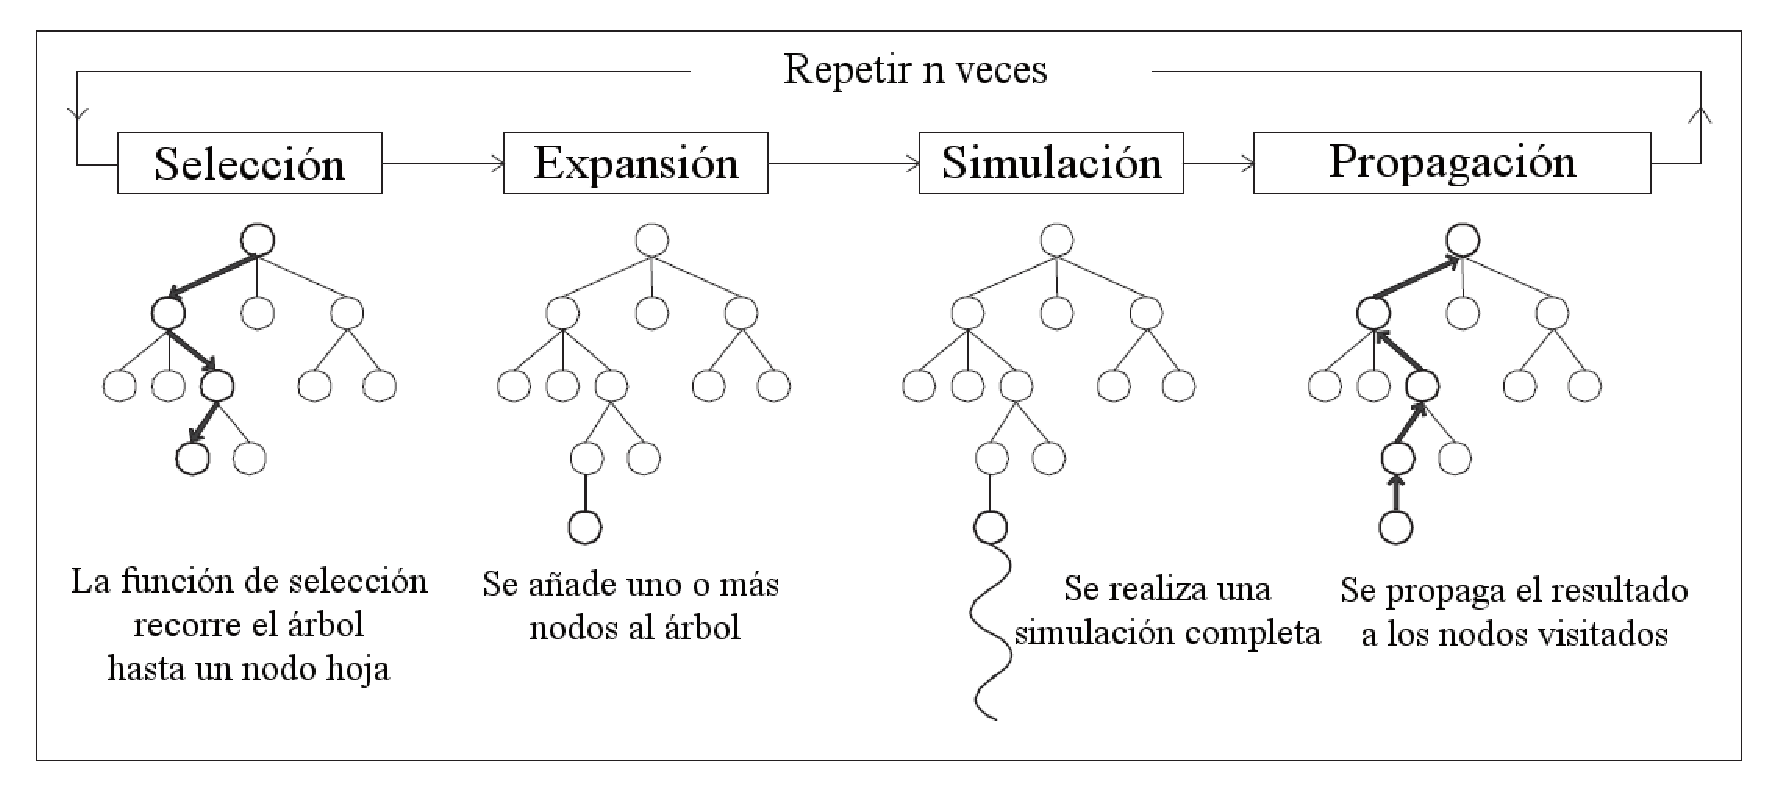
\includegraphics[scale=0.45]{contenido/cap3/imagenes/mcts1.eps}
	\caption[Fases del algoritmo Monte-Carlo Tree Search.]%
	{Fases del algoritmo Monte-Carlo Tree Search. (Imagen adaptada de \citeref{MCTS}.)}
	\label{fig:mcts1}
\end{figure}
La figura~\ref{fig:mcts1} muestra este proceso, que se puede dividir en cuatro fases:
selección, expansión, simulación y propagación.
Antes de detallar cada una de estas fases conviene definir la información que almacenará el árbol MC en cada nodo.

Sea \textit{s} el estado actual, el nodo correspondiente en el árbol MC contiene tres valores:
\begin{itemize}
	\item Número total de simulaciones realizadas desde el estado \textit{s}, que denotamos como \textit{N(s)}.
	\item Número total de simulaciones en las que se selecciona el movimiento \textit{a} desde el estado \textit{s}, que llamamos \textit{N(s,a)}.
	\item El valor Monte-Carlo del estado (valor MC), representado por \textit{Q(s,a)}, es el resultado promedio de todas las simulaciones realizadas en las que se seleccionó el movimiento \textit{a} en el estado \textit{s}:
	\begin{displaymath}
	Q(s,a)=\frac{1}{N(s,a)}\sum_{i=1}^{N(s)}\mathds{I}_i(s,a)z_i
	\end{displaymath}
	donde $z_i$ es el valor de utilidad devuelto por la \textit{i}-ésima simulación, y $\mathds{I}_i(s,a)$ es un indicador que vale 1 si el movimiento \textit{a} fue seleccionado en el estado \textit{s} durante la simulación \textit{i} y 0 en otro caso.
	Nótese que $N(s,a) = \sum_{i=1}^{N(s)}\mathds{I}_i(s,a)$.
\end{itemize}

La información almacenada puede variar dependiendo de la estrategia de selección que se use en la primera fase, aunque aquí se ha usado la información genérica que se puede obtener mediante las simulaciones, es decir, sin emplear conocimiento experto sobre el entorno.

A continuación se detalla cada una de las fases del algoritmo MCTS:
\begin{enumerate}
	\item \textbf{Selección} \\
	Partiendo del estado actual, se realiza una búsqueda en el árbol de juegos hasta encontrar un nodo que no está en el árbol MC.
	Los movimientos realizados en esta búsqueda están elegidos acorde a la información almacenada en el propio árbol MC, siguiendo una determinada estrategia.
	
La estrategia elegida debe mantener un equilibrio entre explotación y exploración.
Se puede seleccionar en cada paso el mejor movimiento, lo que favorecerá la explotación; pero por otro lado, los movimientos menos prometedores todavía tienen que ser explorados a mayor profundidad, debido a la incertidumbre de la evaluación, lo que favorecería la exploración.

En función de la estrategia escogida, obtendremos diferentes versiones del algoritmo MCTS.
Al final de la sección se citan algunas extensiones de MCTS.

Usaremos una estrategia conocida como \textit{optimism in the face of uncertainty}\footnote{Puede traducirse como \textit{optimismo frente a la incertidumbre}.}, que favorece los movimientos con un valor más alto pero permite a su vez explorar aquellas acciones que todavía no han sido suficientemente exploradas.
Para ello, definimos $Q^\oplus(s,a)$ como el valor del movimiento \textit{a} desde el estado actual \textit{s} (valor MC) con una bonificación adicional que será más alta para los movimientos menos visitados:
\begin{displaymath}
Q^\oplus(s,a) = Q(s,a) + c\sqrt{\dfrac{\log N(s)}{N(s,a)}}
\end{displaymath}
donde \textit{c} es una constante de exploración con valores reales en el intervalo [0,1] y \textit{log} es el logaritmo natural (base \textit{e}).

El movimiento elegido, que llamamos $a^\ast$, será aquel que maximize el valor $Q^\oplus(s,a)$:
\begin{displaymath}
a^\ast = \max_a{Q^\oplus(s,a)}
\end{displaymath}

	\item \textbf{Expansión} \\
	Cuando se encuentra un estado que no aparece en el árbol MC, este se añade como un nuevo nodo.
	De esta forma el árbol se expande un nodo en cada simulación.

Una variante puede ser añadir al árbol MC cada estado que se visite en la búsqueda, aunque en la práctica, para reducir los requisitos de memoria, no se añaden todos los nodos en cada simulación.
Normalmente, sólo se añade un nodo al árbol MC en cada simulación: el primer nodo encontrado que no esté presente en el árbol MC.
Si aún así la limitación de la memoria supone un problema, es posible realizar varias simulaciones antes de añadir un nuevo nodo al árbol MC; o incluso podar antiguos nodos del árbol MC a medida que la búsqueda progresa.

	\item \textbf{Simulación} \\
A partir del nuevo estado almacenado en el árbol MC se realiza una simulación completa de la partida siguiendo la estrategia por defecto, esto es, realizando movimientos aleatorios hasta el final del juego.
Después se asigna el valor de utilidad \textit{z} al estado terminal: +1 si es ganador para el jugador, -1 si es perdedor y 0 si es empate.

%En un juego no todos los posibles movimientos tienen la misma probabilidad de jugarse
Obviamente, también puede emplearse en esta fase otra estrategia distinta para elegir los posibles movimientos, como una función heurística que asigne valores más altos a aquellos movimientos que tienen más probabilidad de ser jugados o que parecen más prometedores; pero esta mejora se sale de los objetivos del proyecto por lo que los agentes desarrollados usan la estrategia por defecto para esta fase.

	\item \textbf{Propagación} \\
	Una vez realizada la simulación, se actualiza la información de cada nodo en el árbol MC en función del valor de utilidad obtenido:
	\begin{displaymath}
		\begin{array}{l}
		N(s) \leftarrow N(s) + 1 \\
		N(s,a) \leftarrow N(s,a) + 1 \\ 
		Q(s,a) \leftarrow Q(s,a) + \dfrac{z - Q(s,a)}{N(s,a)} \\
		\end{array}
	\end{displaymath}

\end{enumerate}

El movimiento final seleccionado por MCTS en el estado actual será el movimiento mejor valorado en el árbol MC, es decir, el movimiento \textit{a} con un valor MC mayor.

La figura~\ref{fig:mcts2} muestra cinco simulaciones de MCTS en las que se va construyendo el árbol MC.
Se trata de una versión simplificada del algoritmo. 
Siguiendo con la misma terminología usada en minimax, los nodos de color negro corresponden a nodos \textit{MAX}, los blancos a \textit{MIN}.
Cada simulación obtiene un valor de utilidad (en el caso de la figura~\ref{fig:mcts2} el valor es 1 si gana \textit{MAX} y 0 si gana \textit{MIN}).
En cada simulación se añade un nuevo nodo al árbol y se actualiza el valor de cada nodo en el árbol con el valor de utilidad; también se actualiza el número de veces que se ha seleccionado cada nodo.
\begin{figure}[h]
	\centering
	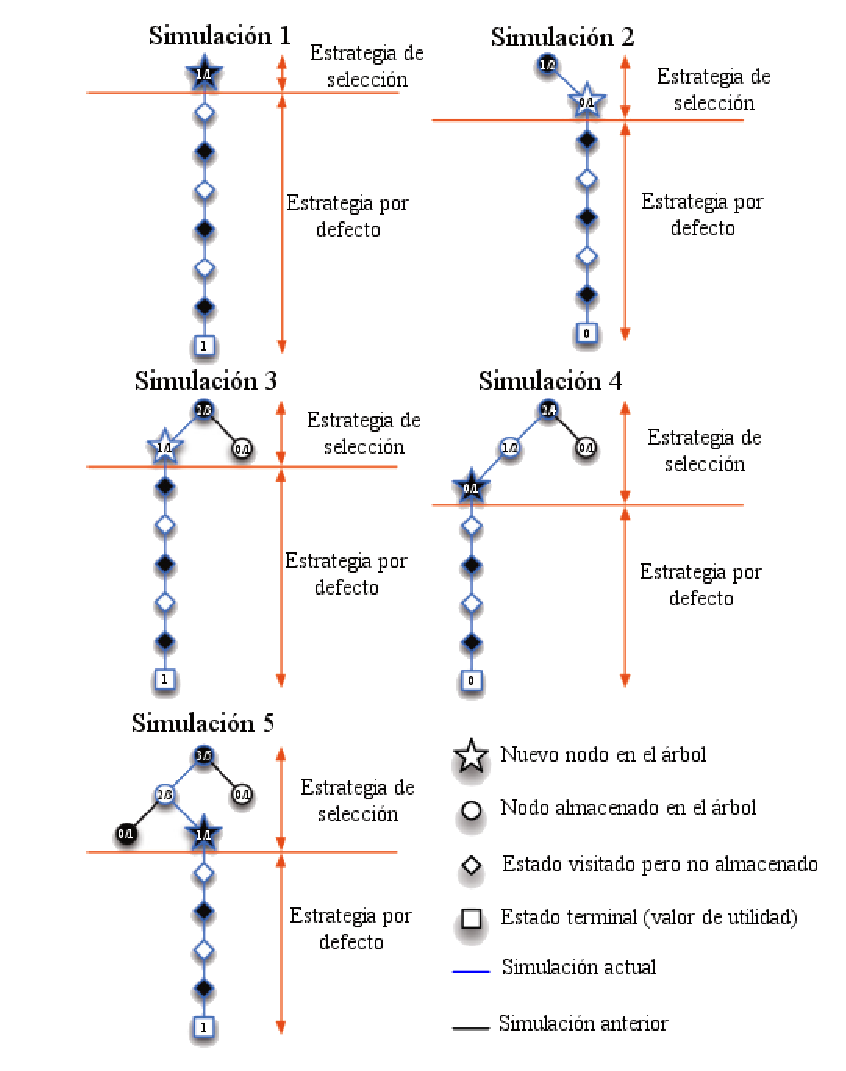
\includegraphics[scale=1]{contenido/cap3/imagenes/mcts2.eps}
	\caption[Cinco simulaciones de Monte-Carlo Tree Search.]%
	{Cinco simulaciones de Monte-Carlo Tree Search. (Imagen adaptada de \citeref{MCTS2}.)}
	\label{fig:mcts2}
\end{figure}
A medida que el árbol MC crece con cada simulación, los valores de los nodos se aproximan al valor minimax real y por tanto la estrategia basada en las simulaciones también se aproxima a la estrategia óptima de minimax.

\clearpage	% le dice a Latex que suelte todas las figuras en una página y comience una página nueva (detallado en los apuntes de los indios).

\bigskip
A continuación se presentan brevemente cuatro extensiones de MCTS en función de la estrategia elegida en las fases de selección y simulación.

\subsubsection{Extensiones de Monte-Carlo Tree Search}
\label{sssec:extensiones_MCTS}
El rendimiento de MCTS puede mejorarse significativamente si se incorpora información del dominio a la estrategia usada en la fase de selección o incluso a la estrategia por defecto usada en la fase de simulación.
Existen varias extensiones de MCTS basadas en la estrategia elegida para ambas fases, algunas extensiones son:
\begin{itemize}
	\item \textbf{\textit{Greedy MCTS}} \\
	La versión más básica de MCTS usa una estrategia \textit{best-first} (primero el mejor) que favorece la explotación frente a la exploración en la fase de selección.
A este algoritmo se le conoce como \textit{greedy MCTS}.
	\item \textbf{Algoritmo \textit{UCT}} \\
	El algoritmo \textit{UCT} (\textit{Upper Confidence bounds applied to Trees}, traducido como \textit{límites superiores de confianza aplicados a los árboles}). 
Usa el principio \textit{optimism in the face of uncertainty} que puede usarse para explorar el árbol de forma eficiente, ya que favorece a los movimientos con mayor valor potencial.
	Nuestra versión MCTS desarrollada se basa en este algoritmo.
	\item \textbf{\textit{Heuristic MCTS}} \\
	Utiliza funciones heurísticas con información del dominio para inicializar los valores de las nuevas posiciones en el árbol MC.
	\item \textbf{\textit{MC-RAVE}} \\
	Utiliza el algoritmo \textit{RAVE} (\textit{Rapid Action Value Estimation}), que mejora el método original compartiendo los valores de diferentes subárboles del árbol MC, por ejemplo en el caso de las transposiciones.
\end{itemize}
\citeref{MCTS2} contiene información detallada sobre estas extensiones de MCTS.

\bigskip
Explicada la estrategia MCTS, se presentan a continuación los agentes que la usan; al igual que ocurrió con el método básico de Monte-Carlo se trata de dos agentes: uno con un número de simulaciones fijado de antemano y otro con un límite de tiempo.

\subsubsection{Monte-Carlo Tree Search con número de simulaciones fijas}
\label{sssec:montecarloTreeSearch_simulaciones}
El primer agente que usa MCTS realiza un número de simulaciones determinado.

Partiendo del estado actual, ejecuta el ciclo de cuatro fases presentado anteriormente tantas veces como indique el número de simulaciones asignado.
Establecer el número de simulaciones en MCTS es aún más difícil que para el agente Monte-Carlo básico porque ahora cada simulación necesita más tiempo para llevarse a cabo debido a que debe gestionar el árbol MC.

Por otro lado, el agente dispone de una opción que permite reutilizar el árbol MC de un movimiento para el siguiente, ya que los valores del árbol son válidos de un movimiento a otro.
Esto permite mejorar la evaluación de los movimientos a medida que el agente juega la partida, a costa de incrementar los recursos necesarios (en memoria y tiempo) para manejar el árbol MC.
Recordemos que el árbol se expande un nodo en cada simulación.

Este agente tiene también un parámetro perteneciente a la constante de exploración \textit{c} que se vio en la fase de selección.
El parámetro permite ajustar la estrategia de selección favoreciendo la exploración (valores próximos a 1) o la explotación (valores próximos a 0).

El último agente también usa MCTS para evaluar el mejor movimiento, pero esta vez dispone de un tiempo limitado para devolver el movimiento.

\subsubsection{Monte-Carlo Tree Search con límite de tiempo}
\label{sssec:montecarloTreeSearch_limiteTiempo}
Este agente usa MCTS con un límite de tiempo para realizar las simulaciones, esto es, las iteraciones completas de cuatro fases de MCTS (selección, expansión, simulación y propagación).

Las iteraciones deben completarse totalmente para que sean válidas; de ahí que asignar el límite de tiempo no sea una tarea trivial.
Si cada iteración necesita más tiempo del disponible, el tiempo límite del agente se extenderá hasta completar la última iteración.
El límite de tiempo viene expresado en segundos al igual que el resto de jugadores con límite de tiempo que se han desarrollado.

Este agente también cuenta con la opción de reutilizar el árbol MC de un movimiento a otro; y también tiene parámetro para ajustar el nivel de exploración en la fase de selección.




% 4. Heurísticos
\chapter{Heurísticos}
\label{cap:heuristicos}
Este capítulo presenta los conceptos de heurístico y evaluador heurístico.
Define la función de evaluación heurística que deben implementar los evaluadores heurísticos que necesitan las estrategias presentadas en el capítulo~\ref{cap:estrategias}.
Se describen dos evaluadores heurísticos que implementan la función de evaluación de forma genérica, mediante tablas de valores y redes neuronales; y se estudiará una forma de entrenarlos con aprendizaje con refuerzo mediante el método de las diferencias temporales.
Estos evaluadores serán en la medida de lo posible, independientes del juego pues no necesitarán información sobre el mismo.
Por último, se presentarán también los evaluadores heurísticos desarrollados específicamente para los juegos del Conecta-4 y del Go.

\bigskip
Un \textbf{heurístico} es una función o algoritmo que nos ayuda a encontrar soluciones ``buenas'' a los problemas.
El heurístico proporciona información que nos permite decidir entre varias alternativas, aunque esta información puede estar incompleta o no ser completamente fiable.
Los heurísticos generalmente se emplean en problemas donde no se puede obtener una solución óptima bajo los requisitos dados de tiempo y espacio. En esos casos nos conformamos con una buena solución.

%En esta sección se describen los evaluadores heurísticos genéricos que emplean los agentes.
%Con genérico queremos decir que son independientes del tipo de juego.
%Los heurísticos genéricos serán aquellos que necesiten de un entrenamiento previo; pues no usan información alguna del dominio.
%Por ello también se estudiará el aprendizaje con refuerzo mediante el método de las diferencias temporales, lo que nos permitirá entrenar a los dos evaluadores heurísticos propuestos: la tabla de valo y la red neuronal.
%Comenzaremos definiendo qué es un heurístico y un evaluador heurístico.

Un \textbf{evaluador heurístico} nos permite evaluar si una situación dada nos es favorable o no, usando para ello una función de evaluación heurística.
El agente presentado en \ref{ssec:evaluador_heuristico} al que llamábamos, valga la redundancia, \textit{Agente evaluador heurístico}, usa un evaluador heurístico para decidir el próximo movimiento.

\bigskip
A continuación se define la función de evaluación heurística, cómo implementar esta función dependerá de cada juego; aunque también se puede implementar de manera genérica para cualquier juego como se verá en las siguientes secciones.

\section{Función de evaluación heurística}
\label{sec:funcion_evaluacion_heuristica}
Este apartado describe las características que deben cumplir las funciones de evaluación heurísticas, de forma que permitan a la estrategia que las use cumplir su objetivo.

\bigskip
Una función de evaluación devuelve una estimación de la utilidad esperada de una posición dada del juego, independientemente de si se trata de una posición final o no.
Por un lado, la función de evaluación debería ordenar los estados terminales del mismo modo que la función de utilidad verdadera del juego.
Por otro lado, para estados no terminales la función de evaluación debería estar fuertemente correlacionada con las posibilidades reales de ganar.
En último lugar, el cálculo no debe emplear demasiado tiempo, ya que la función será invocada repetidas veces por la estrategia para decidir un único movimiento.

La función de evaluación heurística empleada para evaluar los estados de un juego debe devolver un valor positivo si el estado es favorable para nuestro jugador (que llamaremos \textit{MAX} siguiendo la terminología de minimax introducida en \ref{ssec:minimax}), un valor negativo si el estado es desfavorable y cero si el estado es indiferente (no es favorable ni desfavorable).
Este valor será más grande cuanto más favorable sea el estado para \textit{MAX} y más pequeño cuanto más desfavorable sea.
Llamaremos a la función de evaluación \textit{e(n)}, donde \textit{n} es el estado a evaluar:
\begin{equation}
e(n) = \left\{\begin{array}{ll}
\infty & \textnormal{si \textit{n} es un estado terminal y gana \textit{MAX}}\\
>0 & \textnormal{si \textit{n} es favorable para \textit{MAX}}\\
0 & \textnormal{si \textit{n} es indiferente (``empate'')}\\
<0 & \textnormal{si \textit{n} es desfavorable para \textit{MAX}}\\
-\infty & \textnormal{si \textit{n} es un estado terminal y pierde \textit{MAX}}\\
\end{array}\right. \label{eq:heuristico}
\end{equation}

Dos formas de implementar esta función de manera genérica (sin necesitar conocimiento del juego en cuestión) son las tablas de valores y las redes neuronales que darán lugar a nuestros dos evaluadores genéricos.
Para ello es necesario que dispongan de algún tipo de aprendizaje que les permita aprender cuándo un estado es favorable o no.

\bigskip
A continuación se presenta el aprendizaje con refuerzo mediante el método de las diferencias temporales, que será la forma de entrenar a los evaluadores con tablas de valor y redes neuronales.

\section{Aprendizaje con refuerzo}
\label{sec:aprendizaje_refuerzo}
El \textbf{aprendizaje con refuerzo} es un método de aprendizaje automático en el que el algoritmo aprende observando el medio que le rodea.
La información de entrada es el \textit{feedback} o retroalimentación que obtiene del medio como respuesta a sus acciones.
Por lo tanto, el sistema aprende por sí mismo a base de ensayo-error.
Un agente que use aprendizaje con refuerzo necesita saber que algo bueno ha ocurrido cuando gana y que algo malo ha ocurrido cuando pierde.
Esta clase de retroalimentación se denomina \textbf{recompensa} (\textit{reward}).

En este tipo de aprendizaje el agente no tiene ningún conocimiento a priori sobre el entorno, ya que no es necesario.
Lo único que tiene que saber el agente es cuándo ha ganado o ha perdido y puede usar esta información para aprender una función de evaluación que proporcione estimaciones certeras y razonables de la probabilidad de ganar a partir de una situación dada.

En nuestro caso no entrenaremos directamente al agente sino al evaluador heurístico que usa.
El entrenamiento se realizará mediante el método de las diferencias temporales, que se explica a continuación.

\subsection{Método de las diferencias temporales}
\label{ssec:diferencias_temporales}
Llamaremos función de recompensa a la función que indica al evaluador heurístico cuándo ha ganado, ha empatado o ha perdido; y función de utilidad a la función de evaluación que debe aprender y que proporciona la recompensa esperada a partir de una situación dada.

La función de recompensa (R) define el objetivo del problema: obtener la mayor recompensa posible.
Dado un estado, devuelve su valor de recompensa real.
Este valor puede ser por ejemplo un número positivo en caso de que el estado sea ganador, negativo y opuesto si es perdedor y cero si es empate.

La función de utilidad (U) define lo ``deseable'' que es un estado, es decir, su propio valor de recompensa más la utilidad esperada de sus estados sucesores.
Dado un estado, devuelve la recompensa esperada a largo plazo.
La acción o movimiento a elegir en cada momento es la que lleva a un estado de mayor utilidad.

El \textbf{método de las diferencias temporales} (\textit{TD}) consiste en usar las acciones realizadas para ajustar los valores de los estados correspondientes según los valores de recompensa obtenidos.
Se elaboran unas secuencias de entrenamiento, en este caso las secuencias de entrenamiento serán partidas completas de un juego; y partiendo de unos valores iniciales cualesquiera, en cada paso (estado \textit{n} $\rightarrow$ sucesor \textit{s}) de cada secuencia se actualiza el valor de utilidad correspondiente:
\begin{displaymath}
U(n) = U(n) + \alpha(R(n) + U(s) - U(n))
\end{displaymath}
donde $\alpha$ es la tasa de aprendizaje, expresada como un escalar en el intervalo $(0,1)$.
La diferencia de utilidades entre estados sucesivos es la regla de aprendizaje por diferencias temporales y los valores así calculados convergen a las utilidades óptimas de los estados.

En el caso de los juegos el valor inicial de recompensa para un estado es cero.
Por lo que si el valor de utilidad del estado sucesor es menor que el valor del padre, el valor de este último desciende; por el contrario, si el valor de utilidad del estado sucesor es mayor que el valor del padre, el valor de este último aumentará.

Para garantizar que se obtiene una buena estrategia, se pueden realizar movimientos exploratorios durante el entrenamiento.
Para ello se introduce una componente aleatoria para los movimientos del evaluador a entrenar: cada movimiento tendrá una probabilidad de ser aleatorio (exploratorio); en caso de que el movimiento sea exploratorio, no se entrenará al evaluador.

El método de las diferencias temporales se puede aplicar a cualquier juego, pues no necesita de un modelo concreto para llevar a cabo sus actualizaciones; el entorno proporciona las conexiones entre los diferentes estados en forma de movimientos posibles.
Este tipo de aprendizaje es sencillo y no requiere de mucho tiempo de cálculo, pero tiene la desventaja de que el aprendizaje el lento.

\bigskip
Las siguientes secciones describen los evaluadores que implementan la función de evaluación de forma genérica, y que son entrenados empleando aprendizaje con refuerzo mediante el método de las diferencias temporales.

\section{Tabla de Valor}
\label{sec:tabla_valor}
El primer evaluador heurístico que presentamos es la tabla de valor.
Este evaluador implementa la función de evaluación mediante una tabla que almacena el valor de utilidad para cada estado.
El evaluador es entrenado mediante el método de las diferencias temporales; actualizando los valores de la tabla en cada paso del entrenamiento:
\begin{displaymath}
tabla(n) \leftarrow tabla(n) + \alpha(tabla(s) - tabla(n))
\end{displaymath}
donde \textit{n} es el estado cuyo valor se actualiza, \textit{s} es el sucesor del estado \textit{n} elegido y $\alpha$ es la tasa de aprendizaje.

Los valores de utilidad de cada estado al final del entrenamiento se corresponden con el valor de evaluación que devolverá el evaluador para cada estado:
\begin{displaymath}
e(n) = tabla(n)
\end{displaymath}

La ventaja de este evaluador es que es independiente del juego y podrá usarse en cualquiera de los juegos propuestos.
La principal desventaja es la propia tabla de valores, debido al consumo de memoria.

\section{Red Neuronal}
\label{sec:red_neuronal}
El segundo evaluador heurístico es una red neuronal.
Este evaluador implementa la función de evaluación mediante una red neuronal multicapa con el algoritmo de aprendizaje mediante retropropagación.

Para diseñar la arquitectura de la red, se seleccionan una serie de características del entorno.
El número de neuronas de entrada dependerá de las características elegidas, es decir, de cómo se codifiquen los estados de los juegos; lo que implica que este evaluador no pueda ser del todo independiente del juego.\footnote{En \ref{ssec:redNeuronal_conecta4} y \ref{ssec:redNeuronal_go} se definen la funciones de codificación propuestas para los estados del juego del Conecta-4 y del Go.}

La red tiene dos neuronas de salida para realizar la evaluación.
La primera ($p_1$) se interpreta como la probabilidad de que la posición sea ganadora para el primer jugador; y la segunda ($p_2$) como la probabilidad de que la posición sea ganadora para el segundo jugador.
El resultado de la evaluación es la diferencia entre las dos salidas:
\begin{displaymath}
e(n) = p_1 - p_2
\end{displaymath}
donde \textit{n} es el estado evaluado.

La red cuenta con una sola capa intermedia de neuronas.
El número de neuronas de esta capa será un parámetro adicional de la red.
La función que cumple dicha capa intermedia es tratar de realizar una proyección en la que resulten separables linealmente los patrones de entrada de manera que las unidades de salida pueda realizar una clasificación correcta.
Establecer de antemano el número de neuronas intermedias no es sencillo y puede ser necesario realizar varios experimentos antes de encontrar la estructura ideal de la red para un determinado juego.

La forma de entrenar una red neuronal multicapa mediante aprendizaje por refuerzo es un algoritmo conocido como $TD(\lambda)$ (nosotros usaremos la versión simplificada del método TD, visto en el apartado~\ref{ssec:diferencias_temporales}); entrenando la red del siguiente modo: cuando una posición del juego es final, se entrena con la salida correcta (posición ganadora, perdedora o de empate para el jugador); cuando la posición no sea final, se entrena la red para que su evaluación sea parecida a la de la siguiente posición en la secuencia de entrenamiento.

La red dispone también de dos parámetros adicionales para tener un mayor control sobre su aprendizaje.
Por un lado tiene una \textit{tasa de aprendizaje} que permite ajustar la velocidad a la que aprende la red.
Por otro lado tiene un \textit{momento} de entrenamiento que indica la influencia que tendrá la iteración anterior sobre la actual.
Ambos valores son porcentajes expresados mediante escalares en el intervalo $[0,1]$.

%Puede ser necesario un cierto grado de experimentación antes de dar con un red correctamente entrenada.
%Además, pueden presentarse oscilaciones en el aprendizaje de la red.

\section{Heurísticos para el Conecta-4}
\label{sec:heuristicos_conecta4}
En esta sección se define una función heurística que proporciona una evaluación de los estados del juego para el Conecta-4, empleando para ello una matriz de posibilidades.
También se presenta una función de codificación de los estados del juego para un evaluador con red neuronal.

\subsection{Matriz de posibilidades}
\label{ssec:matriz_posibilidades}
Dado un estado del juego la función de evaluación heurística debe devolver un número positivo si el estado es favorable para nuestro jugador, un número negativo si el estado es desfavorable y cero si es indiferente.

Llamaremos a nuestro jugador \textit{MAX} y a su oponente \textit{MIN}.
La función de evaluación para los estados del juego Conecta-4 se define como:
\emph{número de posibilidades de conectar 4 fichas que tiene \textit{MAX}, menos el número de posibilidades de conectar 4 fichas que tiene \textit{MIN}.}

Para determinar el número de posibilidades de conectar 4 fichas se emplea una \textit{matriz de posibilidades}.
A continuación se detalla un método para construir la matriz de posibilidades.
Por simplicidad y sin perder genericidad se considera una versión simplificada del juego: el Conecta-3 sobre un tablero 4x4.

Cada posición del tablero tiene un número de posibilidades distintas de conectar 3 fichas.
La figura~\ref{fig:conecta3_posibilidades1} muestra las posibilidades de conectar 3 fichas que tiene la posición correspondiente a la esquina inferior izquierda del tablero.
Esta posición interviene en tres posibilidades que numeramos del 0 al 2.
La figura~\ref{fig:conecta3_posibilidades2} muestra las posibilidades de conectar 3 fichas que tiene la posición siguiente.
En este caso también tiene tres posibilidades que numeramos del 3 al 5.
\begin{figure}[h]
	\centering
	% Primera imagen
	\begin{minipage}[t]{0.3\linewidth}
		\centering
		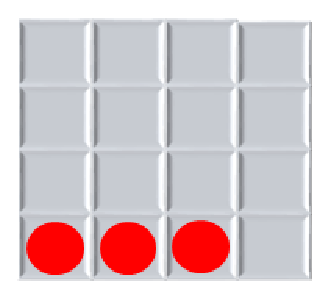
\includegraphics[scale=0.5]{contenido/cap4/imagenes/posibilidadesConecta3_01.eps}
	\end{minipage}
	%\hspace{0.5cm}
	% Segunda imagen
	\begin{minipage}[t]{0.3\linewidth}
		\centering
		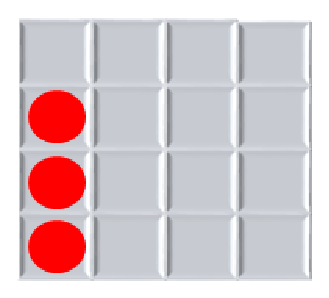
\includegraphics[scale=0.5]{contenido/cap4/imagenes/posibilidadesConecta3_03.eps}
	\end{minipage}
	%\hspace{0.5cm}
	% Tercera imagen
	\begin{minipage}[t]{0.3\linewidth}
		\centering
		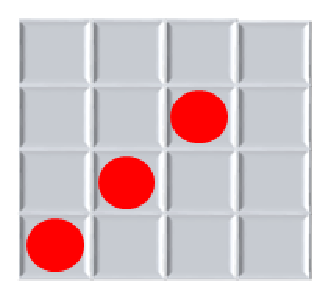
\includegraphics[scale=0.5]{contenido/cap4/imagenes/posibilidadesConecta3_02.eps}
	\end{minipage}
	\caption[Posibilidades en el Conecta-3 (I)]{Posibilidades 0, 1 y 2.}
	\label{fig:conecta3_posibilidades1}
\end{figure}

\begin{figure}[h]
	\centering
	% Primera imagen
	\begin{minipage}[t]{0.3\linewidth}
		\centering
		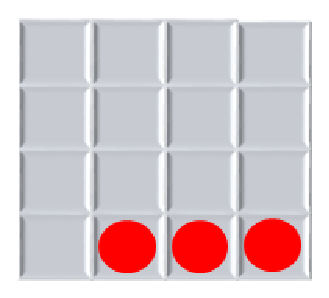
\includegraphics[scale=0.5]{contenido/cap4/imagenes/posibilidadesConecta3_01b.eps}
	\end{minipage}
	%\hspace{0.5cm}
	% Segunda imagen
	\begin{minipage}[t]{0.3\linewidth}
		\centering
		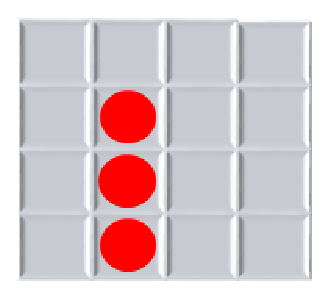
\includegraphics[scale=0.5]{contenido/cap4/imagenes/posibilidadesConecta3_03b.eps}
	\end{minipage}
	%\hspace{0.5cm}
	% Tercera imagen
	\begin{minipage}[t]{0.3\linewidth}
		\centering
		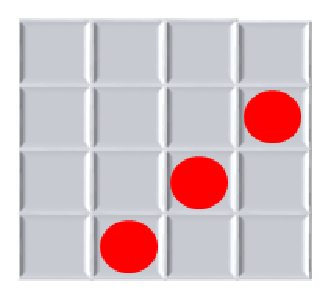
\includegraphics[scale=0.5]{contenido/cap4/imagenes/posibilidadesConecta3_02b.eps}
	\end{minipage}
	\caption[Posibilidades en el Conecta-3 (II)]{Posibilidades 3, 4 y 5.}
	\label{fig:conecta3_posibilidades2}
\end{figure}

Recorriendo todas las posiciones del tablero y enumerando todas las posibilidades en las que interviene cada posición del tablero se obtiene una matriz de posibilidades como la mostrada en la figura~\ref{fig:conecta3_matrizPosibilidades}.

\begin{figure}[h]
	\centering
	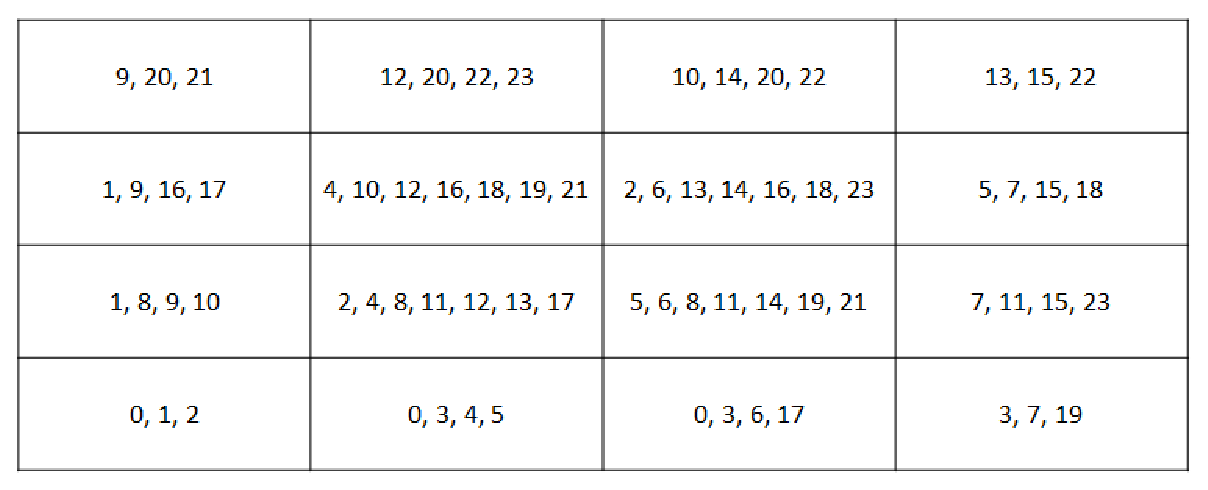
\includegraphics[scale=0.6]{contenido/cap4/imagenes/matrizPosibilidades_Conecta3.eps}
	\caption{Matriz de posibilidades.}
	\label{fig:conecta3_matrizPosibilidades}
\end{figure}

Existen 24 posibilidades de conectar 3 fichas.
Las posiciones menos interesantes del tablero corresponden a las cuatro esquinas.
Las posiciones situadas en las columnas centrales, por el contrario, son las que ofrecen más posibilidades.

Para realizar la evaluación, la función heurística tiene acceso a la matriz de posibilidades del tablero.
Cada jugador dispone de un vector de longitud \textit{n}, donde\textit{ n} es el número de posibilidades de conectar \textit{k} fichas en el tablero.
Para cada casilla ocupada en el tablero se actualizan los vectores adecuadamente con la ayuda de la matriz de posibilidades: si una casilla está ocupada por una ficha de \textit{MAX}, se elimina del vector de \textit{MIN} todas las posibilidades en las que interviene; y si está ocupada por una ficha de \textit{MIN}, se elimina las posibilidades del vector de \textit{MAX}.
El valor devuelto por la función heurística es la diferencia entre la suma de posibilidades libres en el vector de \textit{MAX} y la suma de posibilidades libres en el vector de \textit{MIN}:
\begin{displaymath}
e(n) = posibilidades_{MAX}(n) - posibilidades_{MIN}(n)
\end{displaymath}

\bigskip
A continuación se presenta el evaluador con red neuronal para el Conecta-4, definiendo la función para codificar los estados como entrada a la red.

\subsection{Red neuronal para el Conecta-4}
\label{ssec:redNeuronal_conecta4}
El evaluador con red neuronal presentado en la sección~\ref{sec:red_neuronal} necesitaba de una función de codificación de los estados de los juegos para usarlos como entrada de la red neuronal.

Para los estados del juego del Conecta-4 se codificará cada posición del tablero mediante dos entradas a la red neuronal:
\begin{itemize}
\renewcommand{\labelitemi}{-}
	\item La primera entrada será 1 si hay una ficha del primer jugador y 0 en caso contrario.
	\item La segunda entrada será 1 si hay una ficha del segundo jugador y 0 en caso contrario.
\end{itemize}
De este modo, para un tablero \textit{nxm} se necesitan \textit{2xnxm} entradas en la red neuronal.

El número de neuronas de la capa intermedia no está fijado; lo que permite realizar varias pruebas con diferentes valores hasta encontrar el valor que mejor resultados obtenga.

\bigskip
Una vez definidos los heurísticos específicos para el juego del Conecta-4, presentamos los heurísticos para el juego del Go.

\section{Heurísticos para el Go}
\label{sec:heuristicos_go}
En esta sección se estudiarán varios heurísticos para el juego del Go que permitan decidir si un estado del juego es mejor que otro.

\bigskip
%En la actualidad los computadores juegan al Go a nivel aficionado, debido a que el factor de ramificación para un tablero 19x19 es muy elevado (comenzando en 361).
%Este proyecto estudia una versión reducida en un tablero de 9x9;
%aunque los heurísticos aquí descritos son válidos para cualquier dimensión del tablero.

Las funciones heurísticas están basadas en el objetivo principal del juego: controlar el mayor número de territorios del tablero, entendiendo por territorios el número de intersecciones libres conquistadas por un jugador.
Ubicar piedras juntas ayuda a protegerlas entre sí y evitar ser capturadas. 
Por otro lado, colocar piedras de forma separada hace que se tenga influencia sobre una mayor porción del tablero. 
Parte de la dificultad estratégica del juego surge a la hora de encontrar un equilibrio entre estas dos alternativas. 
Los jugadores pueden jugar tanto de manera ofensiva como defensiva y deben elegir entre tácticas de urgencia y planes a largo plazo más estratégicos.

Teniendo esto en cuenta se definen tres evaluadores heurísticos: uno basado únicamente en los territorios conquistados por cada jugador, y los otros dos en función de los puntos conseguidos por cada jugador hasta el momento, según las reglas de puntuación japonesas para el primer evaluador y según las reglas chinas para el segundo evaluador.

\subsection{Evaluador de territorios}
\label{ssec:evaluador_territorios}
El primer evaluador tiene en cuenta solamente los territorios conquistados por cada jugador.
El valor devuelto por la función heurística para un estado \textit{n} es la diferencia entre el número de territorios pertenecientes a \textit{MAX} y el número de territorios de \textit{MIN}:
\begin{displaymath}
e(n) = territorios_{MAX}(n) - territorios_{MIN}(n)
\end{displaymath}

\subsection{Evaluador de puntos JP}
\label{ssec:evaluador_puntosJP}
El segundo evaluador se basa en la puntuación de cada jugador en el estado actual, según las reglas de puntuación japonesas.
Recordemos que los japoneses cuentan un punto por cada intersección vacía dentro del territorio conquistado menos un punto por cada piedra que haya capturado el enemigo.
El valor de la función heurística para un estado \textit{n} es la diferencia entre los puntos de \textit{MAX} y de \textit{MIN} según las reglas de puntuación japonesas:
\begin{displaymath}
e(n) = puntos_{MAX}^{JP}(n) - puntos_{MIN}^{JP}(n)
\end{displaymath}

\subsection{Evaluador de puntos CH}
\label{ssec:evaluador_puntosCH}
El último evaluador propuesto es igual que el anterior pero teniendo en cuenta las reglas de puntuación chinas.
Los jugadores chinos cuentan un punto por cada intersección vacía dentro del territorio más un punto por cada ficha del jugador sobre el tablero.
Para un estado \textit{n}, el valor de la función heurística es la diferencia de puntos entre \textit{MAX} y \textit{MIN} según las reglas de puntuación chinas:
\begin{displaymath}
e(n) = puntos_{MAX}^{CH}(n) - puntos_{MIN}^{CH}(n)
\end{displaymath}

\bigskip
La siguiente sección presenta el evaluador con red neuronal para el Go, definiendo la función para codificar los estados como entrada a la red.

\subsection{Red neuronal para el Go}
\label{ssec:redNeuronal_go}
Se define a continuación la función de codificación para los estados del Go que necesita la red neuronal como entrada.
El evaluador con red neuronal se presentó en la sección~\ref{sec:red_neuronal} de manera general.

\bigskip
La forma de codificar los estados será la misma que la empleada en el juego del Conecta-4.
Cada posición del tablero se codifica mediante dos entradas a la red neuronal:
\begin{itemize}
\renewcommand{\labelitemi}{-}
	\item La primera entrada será 1 si hay una ficha del primer jugador y 0 en caso contrario.
	\item La segunda entrada será 1 si hay una ficha del segundo jugador y 0 en caso contrario.
\end{itemize}
Para un tablero de \textit{nxn} se necesitan \textit{2xnxn} entradas en la red neuronal.

El número de neuronas de la capa intermedia tampoco está fijado para la red neuronal del Go porque puede ser útil modificar este número en función del tamaño del tablero de juego para encontrar la red neuronal ideal que juegue al Go.


% 5. Especificación
\chapter{Especificación}
\label{cap:especificacion}
En este capítulo se detallan los requisitos del proyecto y se describen los casos de uso de la aplicación interactiva.

\bigskip
El objetivo del proyecto es construir un entorno interactivo que permita jugar y  comparar las diferentes estrategias de juego en IA.
% poner en introducción (objetivos).
%Este entorno interactivo esta basado en una aplicación Java.

\section{Requisitos}
\label{sec:requisitos}
El proyecto puede dividirse en dos partes bien diferenciadas: por un lado el módulo de razonamiento de los agentes junto con los juegos; por otro lado la aplicación interactiva, es decir, la interfaz gráfica de usuario.
Teniendo esto en cuenta se pueden extraer los requisitos de ambas partes de forma separada.

\bigskip
A continuación se presentan primero las características del módulo de razonamiento y después la aplicación gráfica de usuario.

\subsection{Módulo de razonamiento}
\label{ssec:modulo_razonamiento}
El proyecto incluye un módulo de razonamiento para los agentes jugadores y los juegos.

Los algoritmos de decisión deben ser independientes de los propios juegos, es decir, en cada juego debe poder usarse todos los algoritmos disponibles.
Esto es complicado pues hay estrategias que necesitan de información concreta sobre el estado de los juegos para evaluar las posiciones.
Para solucionarlo se separarán también los evaluadores heurísticos de los algoritmos que los usan, independizando totalmente los algoritmos de los juegos.

Los juegos tienen las siguientes características: juegos de dos jugadores, por turnos, de suma cero, de información perfecta y deterministas.
El módulo se completará con la implementación de dos juegos:
\begin{itemize}
\renewcommand{\labelitemi}{$\bullet$}
	\item El juego del Conecta-4; considerando una versión generalizada del mismo con un tamaño de tablero \textit{nxm} y una longitud ganadora de \textit{k} fichas.
	Las pruebas se realizarán sobre tableros de dimensiones 4x4 y 6x7 con longitudes ganadores de tres y cuatro fichas respectivamente.
	\item El juego del Go; considerando una versión generalizada del mismo con un tamaño de tablero \textit{nxn}.
	Las pruebas se realizarán sobre un tablero de dimensiones 9x9.
\end{itemize}
Ambos juegos deben ser representados mediante un espacio de estados que entiendan todos los algoritmos.

Por otro lado, los algoritmos o estrategias deben ajustarse a un espacio de estados genérico, independiente del juego.
Se tratará de versiones generales de los algoritmos, de forma que resulten sencillas de entender.
Los jugadores que se desarrollarán son los presentados a continuación cuyas respectivas estrategias han sido estudiadas en el capítulo~\ref{cap:estrategias}:
\begin{itemize}
\renewcommand{\labelitemi}{$\bullet$}
	\item Un jugador humano, que será el único jugador totalmente dependiente del juego, pues es necesario que pida el movimiento a realizar al usuario mediante un dispositivo de entrada como el teclado o el ratón.
	\item Un jugador con estrategia aleatoria.
	\item Un jugador con evaluador heurístico.
	\item Un jugador con estrategia minimax y una profundidad máxima de búsqueda fijada.
	\item Un jugador con estrategia minimax y un tiempo limitado para realizar la búsqueda.
	\item Un jugador con poda alfa-beta y una profundidad máxima de búsqueda.
	\item Un jugador con poda alfa-beta y un tiempo limitado.
	\item Un jugador con estrategia minimax y una profundidad máxima de búsqueda que incluye además una tabla de transposición.
	\item Un jugador con estrategia minimax y un tiempo limitado que incluye además una tabla de transposición.
	\item Un jugador con poda alfa-beta y una profundidad máxima de búsqueda que incluye también una tabla de transposición.
	\item Un jugador con poda alfa-beta y un tiempo limitado que incluye también una tabla de transposición.
	\item Un jugador que utiliza el método de Monte-Carlo para decidir el mejor movimiento realizando un número determinado de simulaciones.
	\item Un jugador que utiliza el método de Monte-Carlo con un límite de tiempo para realizar las simulaciones.
	\item Un jugador que utiliza el método Monte-Carlo Tree Search para decidir el mejor movimiento realizando un número determinado de simulaciones.
	\item Un jugador que utiliza el método Monte-Carlo Tree Search con un límite de tiempo para realizar las simulaciones.
\end{itemize}

La tabla \ref{tab:agentes_parametros} muestra de forma resumida todas las estrategias junto con los parámetros permitidos.
{\footnotesize
\begin{table}[!h]
\caption{Estrategias y sus parámetros.}
\label{tab:agentes_parametros}	% La etiqueta debe ir justo despues de caption o dentro de él.
\begin{center}
\begin{tabular}{lp{2cm}p{2cm}p{2cm}p{2cm}}
\hline
 & \multicolumn{4}{c}{\textbf{Parámetros}}\\
\textbf{Estrategias} & Prof. máx. búsqueda & Nº simulaciones & Límite tiempo & Heurísticos\\
\hline
Aleatoria &  & & & \\
Evaluador heurístico & & & & \checkmark \\ 
Minimax & \checkmark & & \checkmark & \checkmark \\
Alfa-Beta & \checkmark & & \checkmark & \checkmark \\ 
Minimax (tabla de transposición) & \checkmark & & \checkmark & \checkmark \\ 
Alfa-Beta (tabla de transposición) & \checkmark & & \checkmark & \checkmark \\
Monte-Carlo & & \checkmark & \checkmark & \\
Monte-Carlo Tree Search & & \checkmark & \checkmark  & \\
\hline
\end{tabular}
\end{center}
\end{table}
}

Los evaluadores heurísticos que necesitan algunos de los jugadores son independientes de estos últimos como se comentó anteriormente.
Los evaluadores heurísticos que se incluirán son:
\begin{itemize}
\renewcommand{\labelitemi}{$\bullet$}
	\item Un evaluador para el Conecta-4 basado en una matriz de posibilidades.
	\item Un evaluador para el Go basado el número de territorios conquistados.
	\item Un evaluador para el Go basado en los puntos según las reglas japonesas.
	\item Un evaluador para el Go basado en los puntos según las reglas chinas.
	\item Un evaluador que emplea una tabla de valor.
	\item Un evaluador que emplea una red neuronal.
\end{itemize}
Los dos últimos evaluadores (tabla de valor y red neuronal) necesitan de un entrenamiento previo; por lo que se incluirá un módulo de aprendizaje que permita entrenar dichos evaluadores.

El módulo de razonamiento debe proporcionar un marco de trabajo de forma que permita modificar o añadir nuevos algoritmos, juegos y heurísticos de manera independiente y sencilla.

\bigskip
A continuación se detallan los requisitos de la aplicación interactiva que hará uso del módulo de razonamiento de los algoritmos y juegos.

\subsection{Aplicación interactiva}
\label{ssec:aplicacion_interactiva}
El proyecto incluye una aplicación interactiva basada en una interfaz gráfica de usuario. 
La aplicación integra el módulo de razonamiento de los algoritmos y juegos dando acceso a toda su funcionalidad.

La aplicación permite al usuario seleccionar un juego disponible y configurar sus parámetros, como el tamaño del tablero.
También permite seleccionar la estrategia a usar por cada jugador, configurando a su vez los parámetros de la estrategia en cuestión, como por ejemplo los evaluadores heurísticos o el tiempo disponible para realizar la jugada.
En el caso de los evaluadores heurísticos que lo necesiten, la aplicación ofrece la posibilidad de entrenarlos configurando los diferentes aspectos del entrenamiento (número de partidas, oponente, pruebas, etc.).

Una vez seleccionado el juego y los jugadores, la aplicación permite jugar, ver el desarrollo de una partida, simular varias partidas o analizar estados.
Al finalizar cada una de estas acciones, la aplicación muestra estadísticas sobre las mismas y ofrece la opción de generar un informe con las estadísticas.

La aplicación también cuenta con un sistema de ayuda que proporciona información sobre los componentes visuales cuando el usuario se sitúa sobre ellos.

\bigskip
A partir de estos requisitos, la siguiente sección detalla los principales casos de uso de la aplicación.

\section{Casos de uso}
\label{sec:casos_uso}
La aplicación interactiva cuenta principalmente con tres casos de uso: jugar, simular y analizar estado, que se muestran en el diagrama de la figura~\ref{fig:casos_uso_principales}.
El actor principal de todos los casos de uso es el usuario de la aplicación.
\begin{figure}[h]
	\centering
	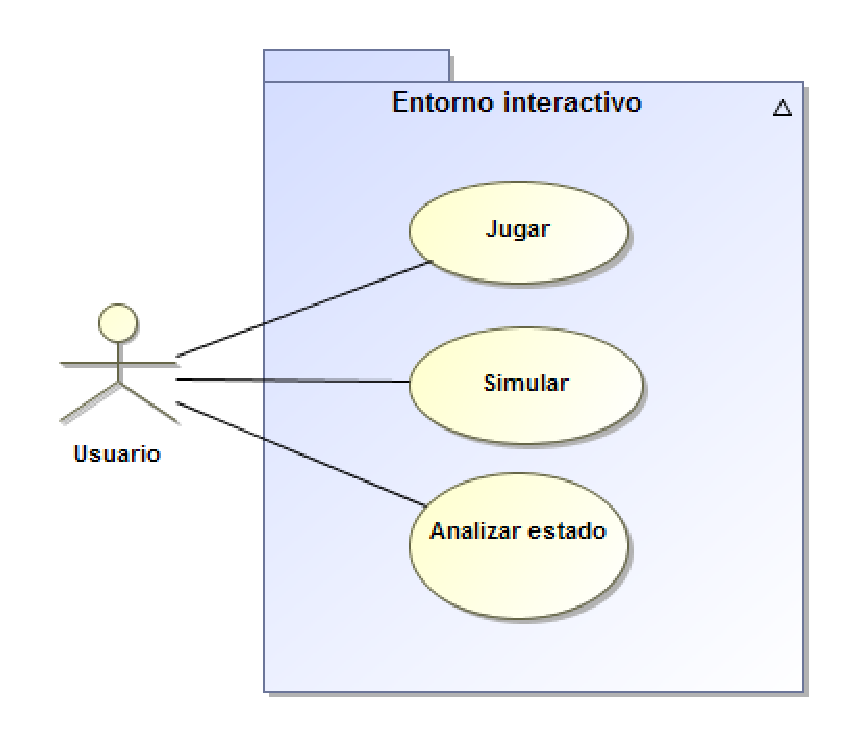
\includegraphics[scale=0.5]{contenido/cap5/imagenes/principales.eps}
	\caption{Diagrama de los principales casos de uso de la aplicación.}
	\label{fig:casos_uso_principales}
\end{figure}
\begin{enumerate}
	\item \begin{description}
		\item \textbf{Caso de uso:} Jugar\\
		El usuario juega una partida al juego elegido con los jugadores seleccionados. 
		\item \textbf{Extensión:} Si ninguno de los jugadores es humano, se muestra el desarrollo de la partida entre los jugadores controlados por el ordenador.
	\end{description}
	\item \begin{description}
		\item \textbf{Caso de uso:} Simular\\
		El usuario indica un número de partidas y la aplicación juega las partidas entre los dos jugadores seleccionados. El desarrollo de las partidas no se muestra. 
		\item \textbf{Precondición:} Ambos jugadores deben ser controlados por el ordenador, en caso contrario la opción de simular estará desactivada.
	\end{description}
	\item \begin{description}
		\item \textbf{Caso de uso:} Analizar estado\\
		El usuario crea un estado concreto del juego elegido, colocando manualmente las fichas sobre el tablero. A partir de ese estado, los jugadores seleccionados realizan independientemente un único movimiento cada uno.
		\item \textbf{Precondición:} Ambos jugadores deben ser controlados por el ordenador, en caso contrario la opción de analizar estado estará desactivada.
	\end{description}
\end{enumerate}
Cada uno de estos casos de uso produce unas estadísticas diferentes que son mostradas al finalizar los mismos.
Parte de esta información depende del jugador seleccionado; cada estrategia proporciona sus propias estadísticas, que son independientes del caso de uso elegido.
La aplicación permite además generar un informe en texto plano con toda la información de las estadísticas obtenidas.
Una vez terminado un caso de uso, los jugadores se pueden reutilizar para iniciar otro caso de uso sin tener en cuenta las estadísticas anteriores; lo que permite realizar tantas pruebas como se desee.

A continuación se presentan los casos de uso pertenecientes a la selección y configuración de los juegos y de las estrategias.
Para los juegos tenemos un único caso de uso (seleccionar juego) con la opción de modificar sus parámetros. La figura~\ref{fig:casos_uso_juegos} muestra el diagrama para este caso de uso.

\begin{figure}[b]
	\centering
	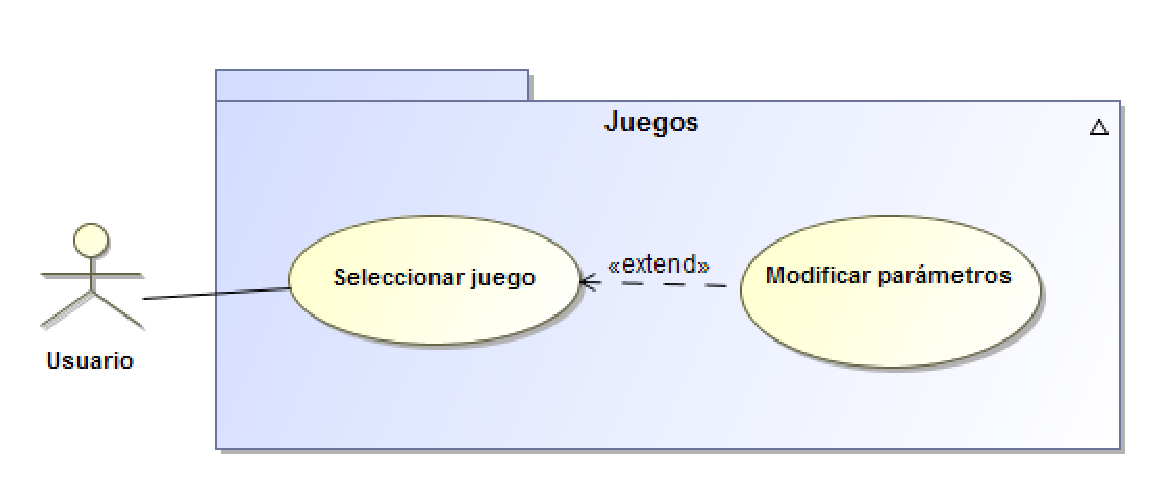
\includegraphics[scale=0.5]{contenido/cap5/imagenes/seleccionarJuego.eps}
	\caption{Diagrama de casos de uso para los juegos.}
	\label{fig:casos_uso_juegos}
\end{figure}

\begin{enumerate}[resume]
%\renewcommand{\labelitemi}{$\bullet$}
%\renewcommand{\labelitemii}{-}
	\item \begin{description}
		\item \textbf{Caso de uso:} Seleccionar juego \\
		El usuario elige el juego deseado de entre los disponibles.	
		\item \textbf{Extensión:} El usuario configura el juego seleccionado. Los parámetros a configurar dependen del juego:
		\begin{itemize}
	\item Conecta-4: El usuario elige el tamaño del tablero y la longitud ganadora de fichas.
	\item Go: El usuario elige el tamaño del tablero, las reglas de puntuación y los puntos de ventaja para el segundo jugador.
	\end{itemize}
	\end{description}
\end{enumerate}

En el caso de las estrategias, existen dos casos de uso: uno para seleccionar la estrategia del primer jugador y otro para seleccionar la estrategia del segundo jugador.
El escenario principal de ambos casos de uso es idéntico, por lo que sólo se describe uno de forma general. 
El diagrama de la figura~\ref{fig:casos_uso_estrategias} muestra el caso de uso de forma genérica para ambos jugadores.
\begin{figure}[h]
	\centering
	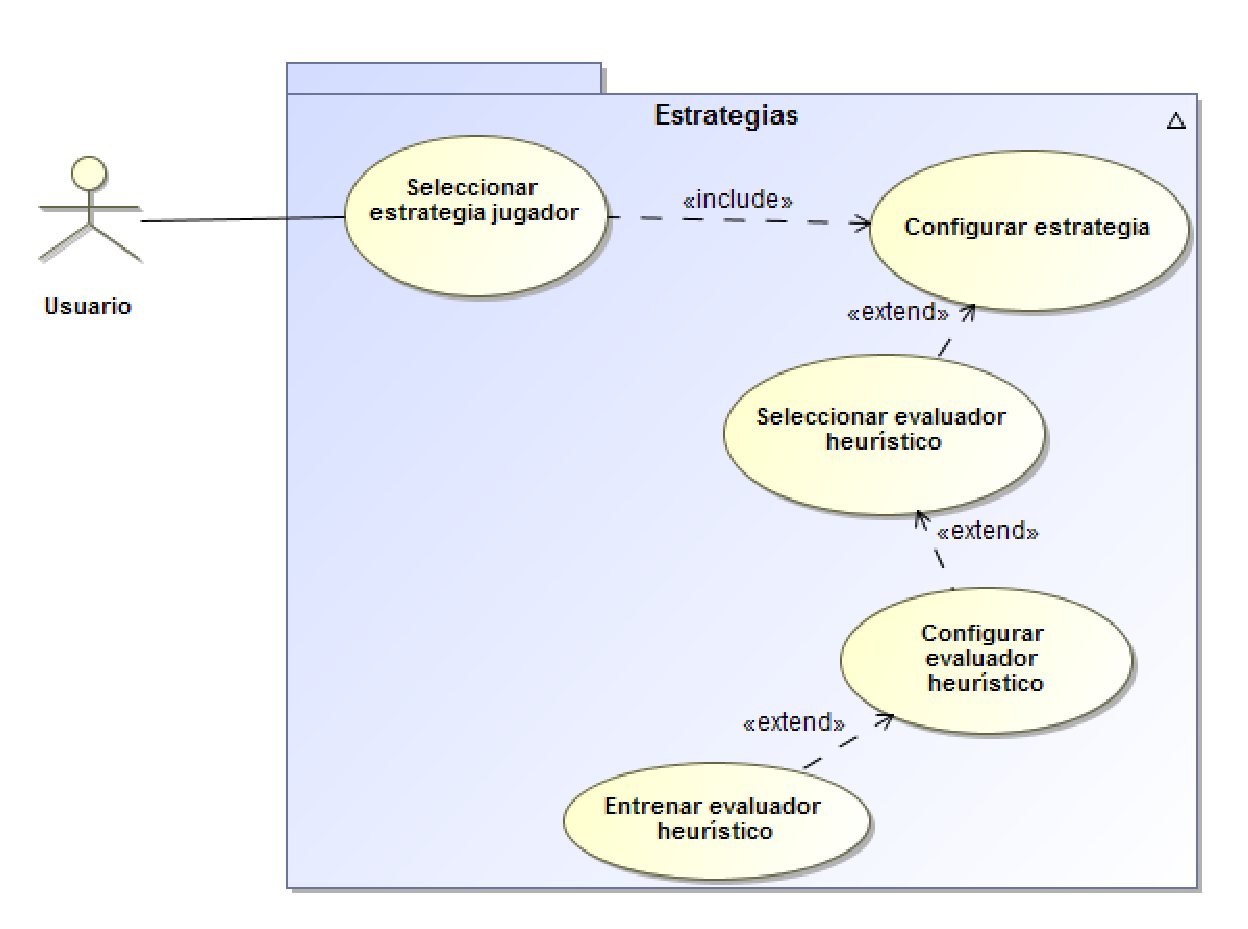
\includegraphics[scale=0.5]{contenido/cap5/imagenes/seleccionarEstrategia.eps}
	\caption{Diagrama de casos de uso para las estrategias.}
	\label{fig:casos_uso_estrategias}
\end{figure}
\begin{enumerate}[resume]
	\item \begin{description}
		\item \textbf{Caso de uso:} Seleccionar estrategia del jugador \\
		El usuario selecciona y configura los parámetros de la estrategia para uno de los jugadores.
		\item \textbf{Precondición:} El usuario ha seleccionado un juego.
		\item \textbf{Extensiones:}\\
		\begin{enumerate}
		 \renewcommand{\labelenumii}{\arabic{enumi}\alph{enumii}.}  
		 \renewcommand{\labelenumiii}{\arabic{enumi}\alph{enumii}.\arabic{enumiii}.}
		 \renewcommand{\labelenumiv}{\arabic{enumi}\alph{enumii}.\arabic{enumiii}\alph{enumiv}.}
			\item El usuario selecciona un evaluador heurístico.
			\begin{enumerate}
				\item El usuario configura el evaluador heurístico seleccionado.
				\begin{enumerate}
					\item El usuario configura el entrenamiento y la aplicación entrena el evaluador heurístico.
				\end{enumerate}				 
			\end{enumerate}
		\end{enumerate}
	\end{description}
\end{enumerate}
 

% 5. Arquitectura de la aplicación (diseño)
\chapter{Arquitectura de la aplicación}
\label{cap:diseno}
Este capítulo presenta la arquitectura del sistema.
Describe el diseño del módulo de razonamiento y muestra los diagramas de clases correspondientes.
También se presentan brevemente el diseño de la interfaz de la aplicación con los patrones de diseño usados en la misma.

% PARA DISEÑO
%%Figura~\ref{fig:sistema} 
%muestra un esquema de la arquitectura del sistema.
%Se observa la base del sistema constituida por el marco de trabajo dividido en dos partes principales relacionadas: Estrategias y Juegos, que definen las interfaces que deben implementar las estrategias y los juegos que se quieran desarrollar.
%Este incluye también el entorno de usuario interactivo y otros componentes estándar para el dominio de los juegos en IA.
%
%Las distintas implementaciones de estrategias y juegos no forma parte del marco de trabajo, lo que permite ampliar el número de estrategias y juegos del sistema.
%
%

%La siguiente sección describe la arquitectura del módulo de razonamiento.

\section{Módulo de razonamiento}
\label{sec:arquitectura_modulo_razonamiento}
El módulo de razonamiento se ha dividido en tres módulos más pequeños: el módulo de los juegos, el de los jugadores o estrategias y el de los heurísticos.
Todos los módulos se encuentran relacionados mediante unas interfaces definidas.
A continuación se describen en detalle cada uno de estos módulos.

\subsection{Juegos}
\label{ssec:arquitectura_juegos}
En el capítulo~\ref{cap:juegos} se definió formalmente un juego como una clase de problemas de búsqueda que contiene: un estado inicial, una función sucesor, un test terminal y una función de utilidad o función objetivo.
Definiendo una interfaz adecuada se puede construir un módulo que permita implementar fácilmente cualquier juego del tipo considerado.

La figura~\ref{fig:diagramaclases_juegos} muestra el diagrama de clases del módulo de juegos junto con los dos juegos considerados (Conecta-K y Go).
Para simplificar el diagrama no se muestra la implementación de ambos juegos, sino únicamente la relación existente entre ellos y el módulo de juegos.

\begin{figure}[!p]
	\centering
	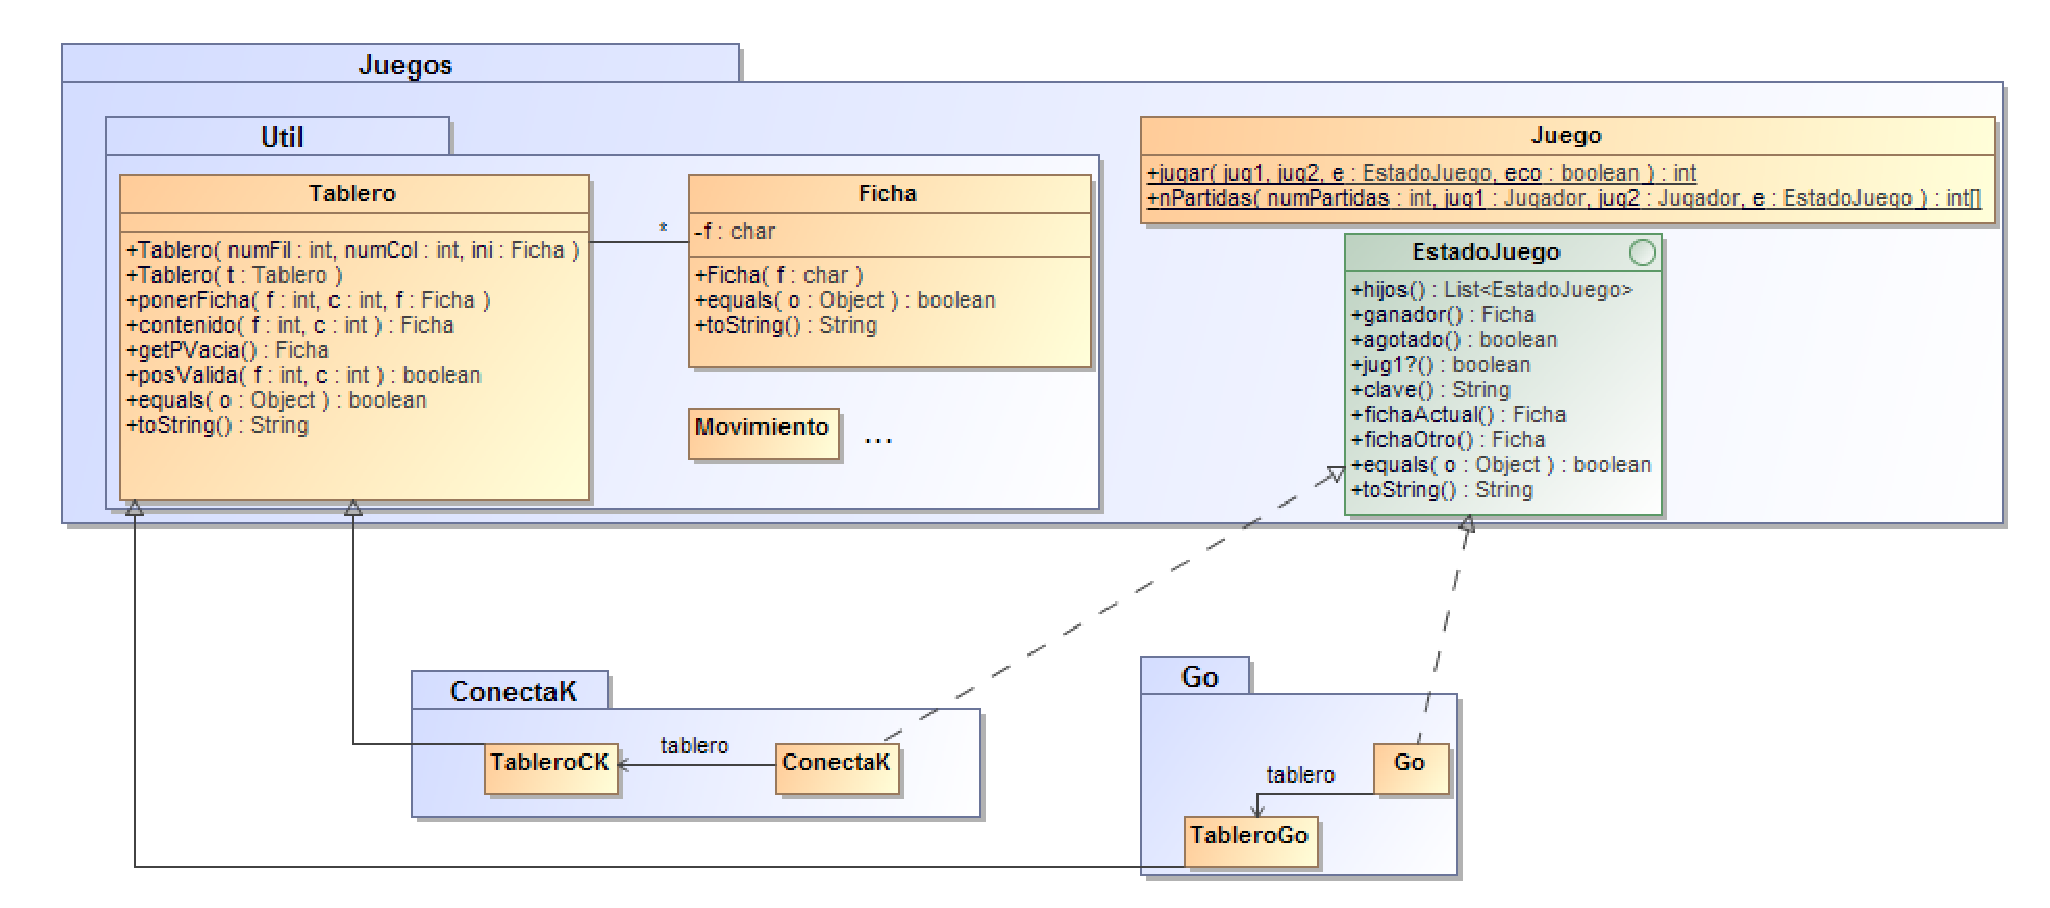
\includegraphics[scale=0.5,angle=90]{contenido/cap6/imagenes/diagramaclases_juegos.eps}
	\caption{Diagrama de clases de los juegos.}
	\label{fig:diagramaclases_juegos}
\end{figure}

El elemento principal del módulo de juegos es la interfaz \texttt{\textit{EstadoJuego}}, que proporciona una representación de los estados de un juego.
Se trata del elemento más importante de todo el módulo de razonamiento: cualquier juego debe implementar esta interfaz para representar sus estados.
La interfaz contiene una función sucesor (método \texttt{hijos}), un test terminal (\texttt{agotado}), y métodos que permiten indexar el estado en una posible estructura, conocer el ganador (si lo hay) y el jugador al que le toca jugar, comparar dos estados y proporcionar una descripción del estado.

Esta representación permite obtener el árbol de juegos a partir un estado gracias al método \texttt{hijos} que devuelve los sucesores inmediatos del estado actual.

Nótese que la interfaz no proporciona una función de utilidad para los estados terminales, ya que el método ganador sólo indica quién ha ganado.
El valor de utilidad al final de una partida se ha diseñado de manera independiente del juego: el método estático \texttt{jugar} de la clase \texttt{Juego} permite jugar una partida entre dos jugadores a partir de un estado inicial y devuelve el valor de utilidad obtenido (1 si gana el primer jugador, -1 si gana el segundo jugador y 0 en caso de empate).
Igualmente el método \texttt{nPartidas} juega un número determinado de partidas devolviendo los valores de utilidad de cada partida.

El módulo también proporciona un paquete de utilidades que ayuda a implementar los juegos como un tablero genérico, fichas o una representación de los movimientos.

El diagrama de la figura~\ref{fig:diagramaclases_juegos} sólo muestra en los paquetes \texttt{ConectaK} y \texttt{Go} las clases que representan a dichos juegos.
Estos paquetes son independientes del módulo de juegos y contienen otras clases como evaluadores heurísticos específicos para cada juego o jugadores dependientes del juego como el jugador humano.

\bigskip
El siguiente apartado muestra el diseño del módulo correspondiente a las estrategias.

\subsection{Estrategias}
\label{ssec:arquitectura_estrategias}
El módulo de estrategias se muestra en el diagrama de la figura~\ref{fig:diagramaclases_estrategias}.

\begin{figure}[!p]
	\centering
	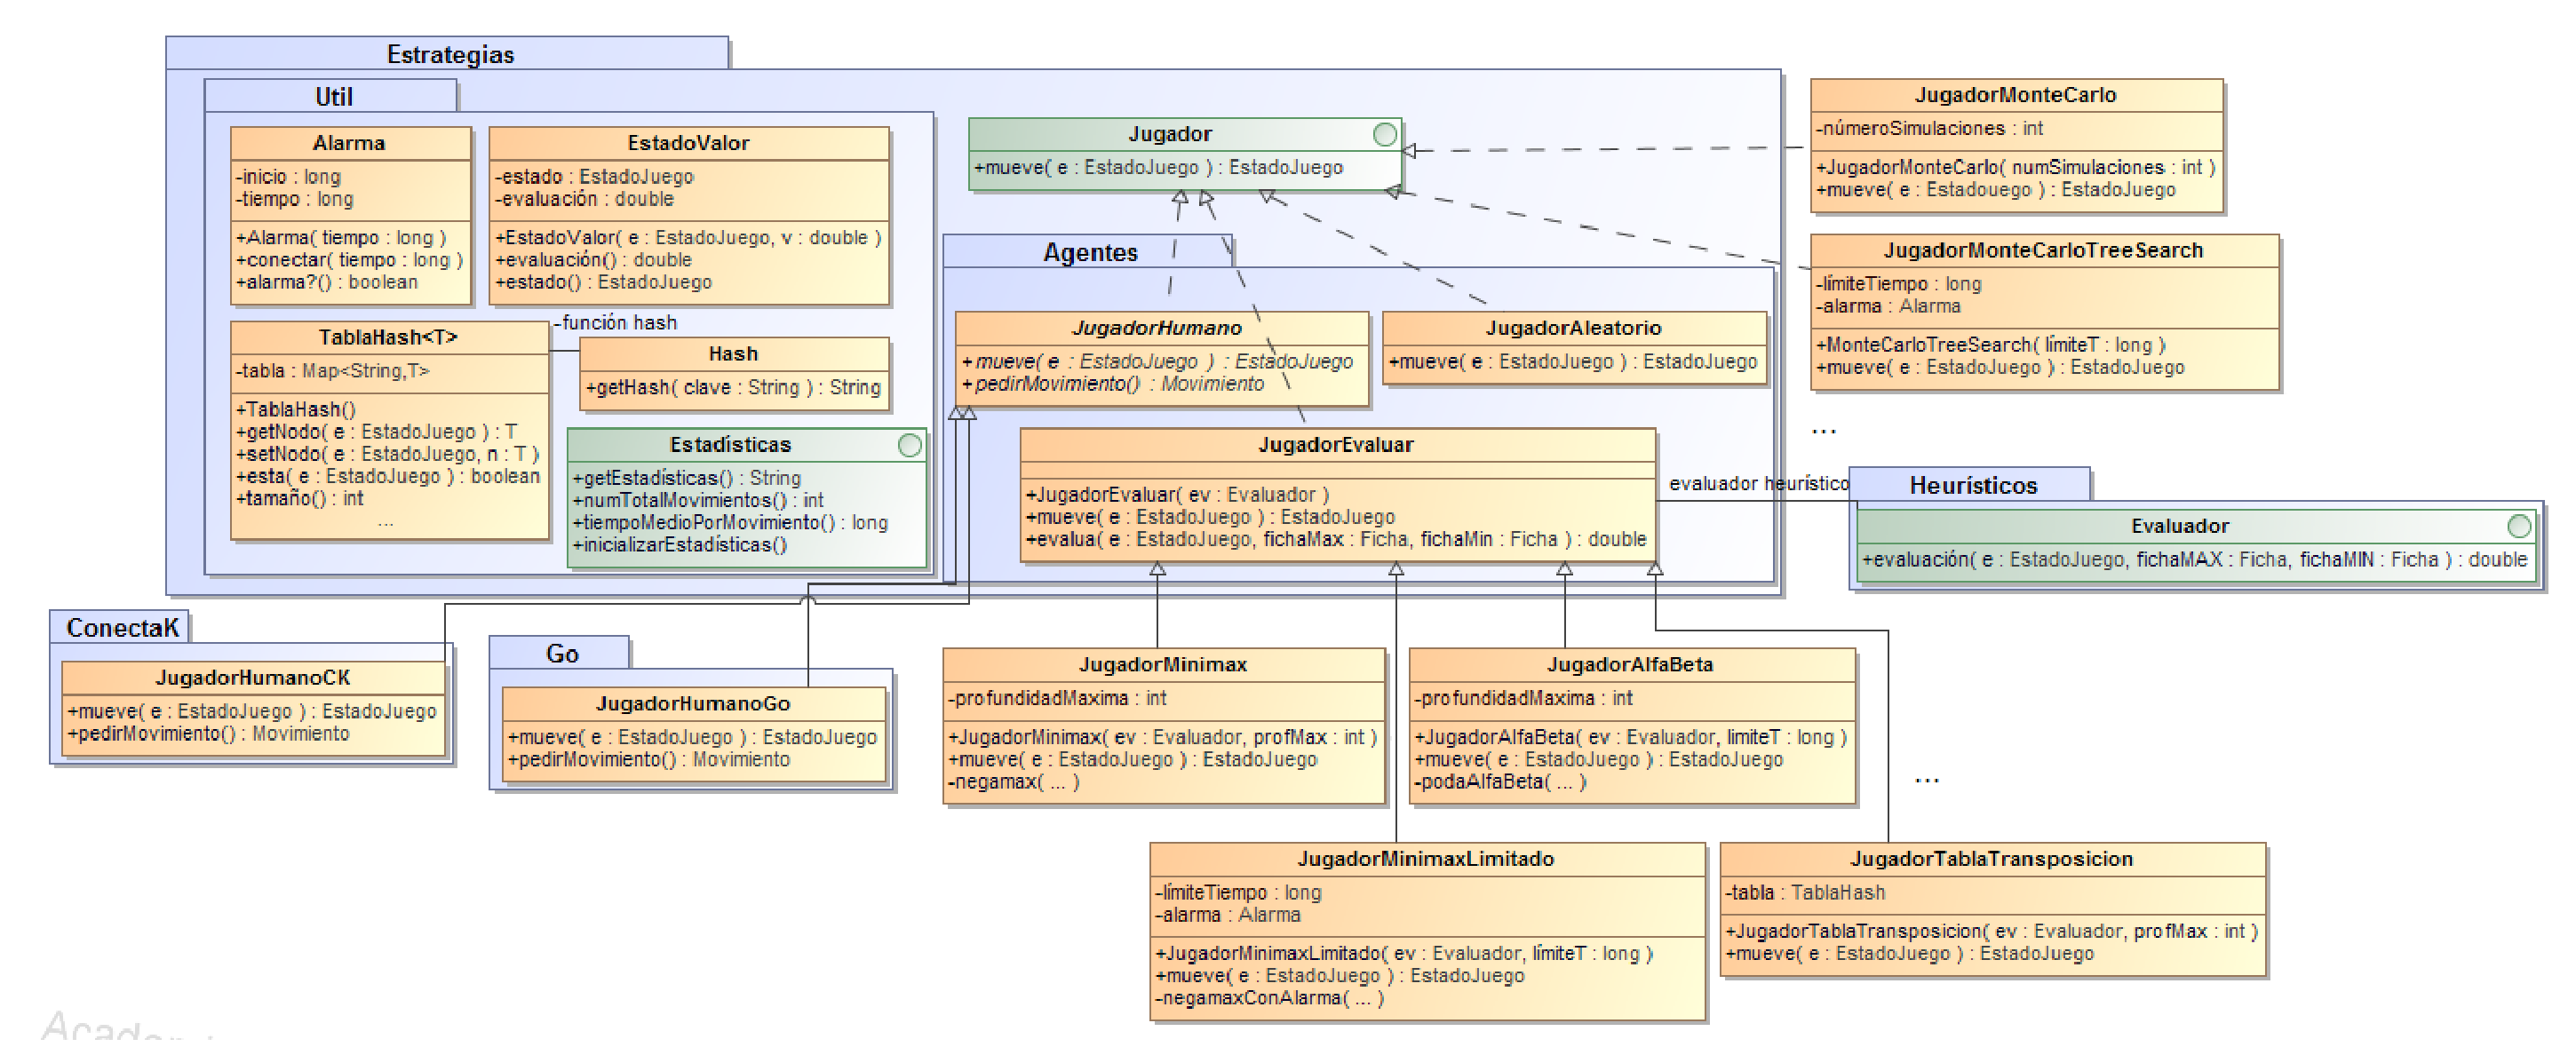
\includegraphics[scale=0.4,angle=90]{contenido/cap6/imagenes/diagramaclases_estrategias.eps}
	\caption{Diagrama de clases de las estrategias.}
	\label{fig:diagramaclases_estrategias}
\end{figure}

Toda clase que represente un agente jugador debe implementar la interfaz \texttt{\textit{Jugador}}.
Esta interfaz solamente tiene un método (\texttt{mueve}) que devuelve el estado resultante de que el jugador mueva en el estado actual dado.

El \texttt{JugadorAleatorio} implementa esta interfaz de forma general lo que le permite jugar a cualquier tipo de juego.
No ocurre lo mismo con el \texttt{JugadorHumano}, que necesita pedir el movimiento a realizar mediante un dispositivo de entrada, de ahí que se trate de una clase abstracta.
Cada juego debe implementar su propio jugador humano.

El \texttt{JugadorEvaluar} necesita de un evaluador heurístico que proporciona la evaluación de los estados; toda estrategia que necesite de un heurístico se considera una especialización de este jugador.
El resto de jugadores no forman parte del paquete \texttt{Estrategias} porque cada jugador puede implementar su estrategia de forma diferente, por ejemplo, la estrategia minimax se puede implementar siguiendo la definición \ref{eq:minimax} o mediante el algoritmo negamax (\ref{sssec:negamax}).
En el diagrama, por simplicidad, no aparecen todos las estrategias desarrolladas.

También se proporciona un paquete de utilidades para las estrategias que necesiten de una alarma de tiempo, una tabla hash o una función hash\footnote{La función hash implementada realiza una codificación mediante el algoritmo de reducción criptográfico \textit{MD5}\citeref{rfc1321}.}.
Para simplificar el diagrama tampoco se muestran explícitamente las asociaciones entre los jugadores y las utilidades usadas por cada uno.
Destaca la interfaz \texttt{\textit{Estadísticas}} que deberán implementar las estrategias que deseen proporciona sus propias estadísticas.

\bigskip
A continuación se detalla el módulo de los heurísticos.

\subsection{Heurísticos}
\label{ssec:arquitectura_heuristicos}
El módulo de heurísticos contiene las definiciones de los objetos evaluadores y permite entrenarlos mediante aprendizaje por refuerzo.
La figura~\ref{fig:diagramaclases_heuristicos} muestra en el diagrama de este módulo.

\begin{figure}[!p]
	\centering
	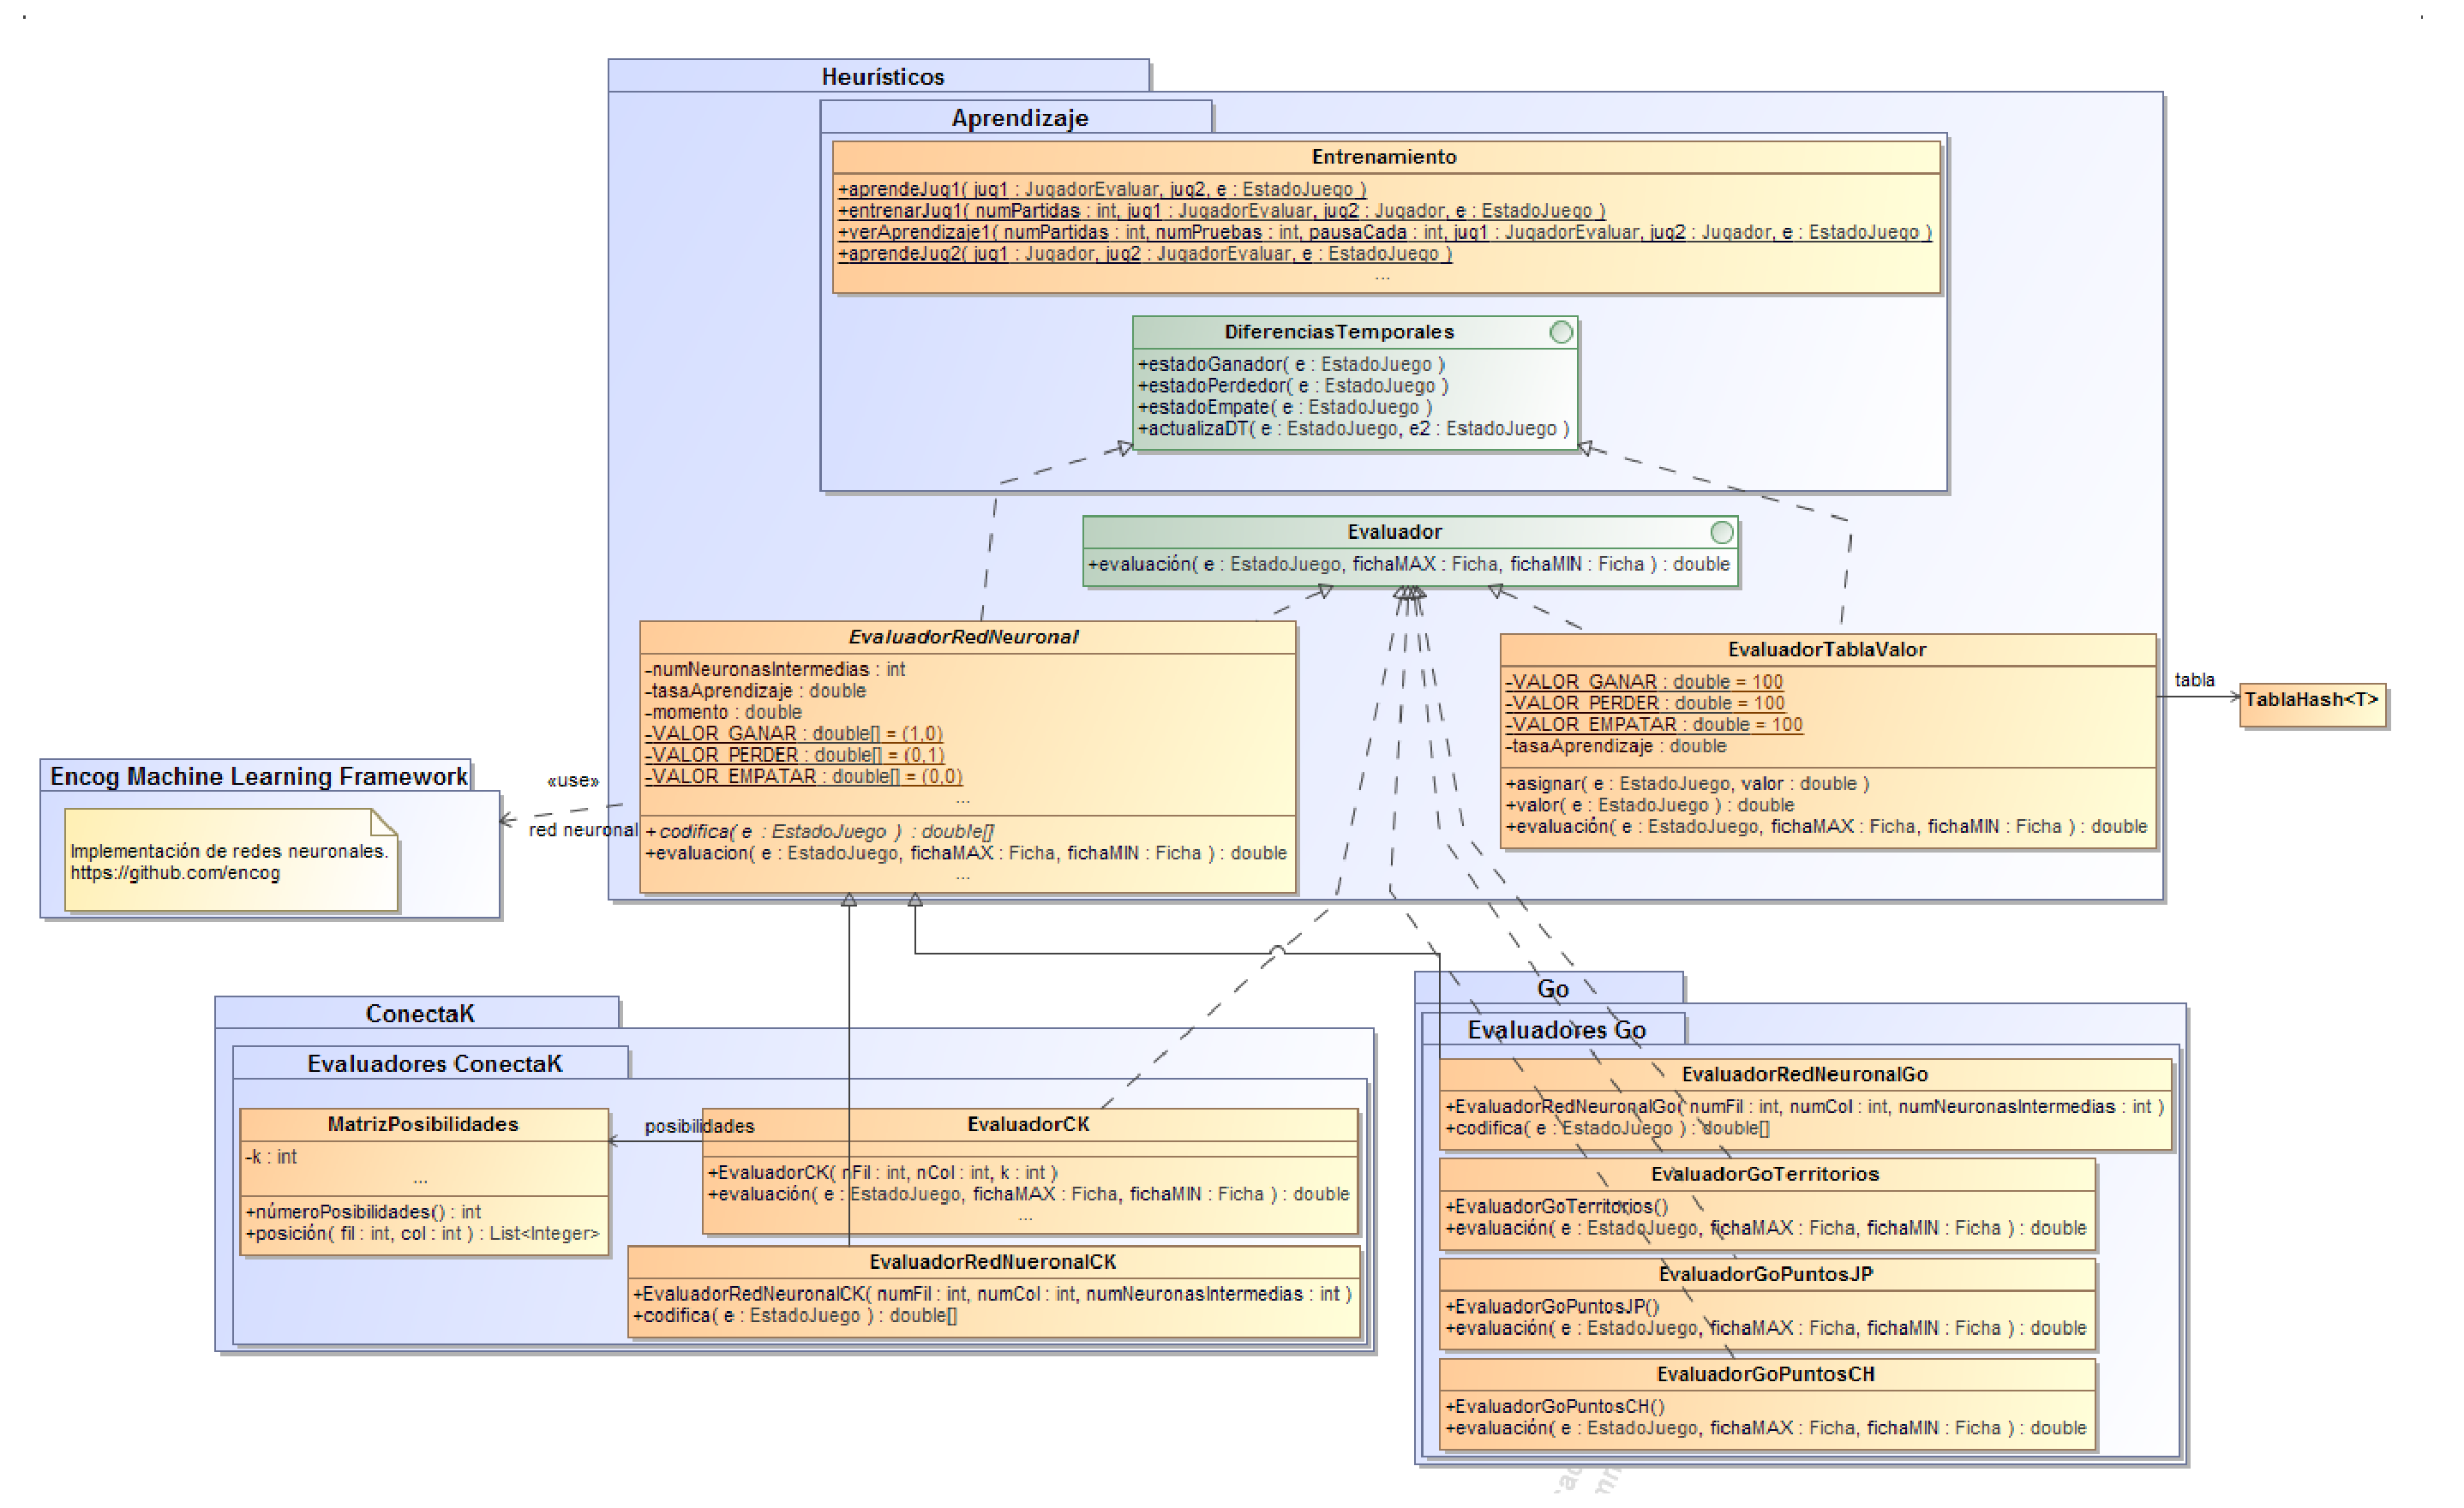
\includegraphics[scale=0.4,angle=90]{contenido/cap6/imagenes/diagramaclases_heuristicos.eps}
	\caption{Diagrama de clases de los heurísticos.}
	\label{fig:diagramaclases_heuristicos}
\end{figure}

La interfaz \texttt{\textit{Evaluador}} representa los objetos evaluadores heurísticos que proporcionan el valor de evaluación de un estado.
El juego que quiera proporcionar un heurístico para sus estados debe implementar esta interfaz siguiendo la definición de la función de evaluación heurística dada en~\ref{eq:heuristico}.

El módulo ofrece un paquete para definir evaluadores entrenables mediante aprendizaje por refuerzo; para ello los evaluadores deben implementar la interfaz \texttt{\textit{DiferenciasTemporales}}.
La clase \texttt{Entrenamiento} permite entrenar a los jugadores.
Debido a que los valores aprendidos por el evaluador son diferentes según se trate del primer jugador o del segundo, la clase proporciona métodos diferentes para entrenar al primer jugador, al segundo jugador o a ambos jugadores simultáneamente; para simplificar el diagrama, no se muestran todos estos métodos, pero sus cabecera son idénticas a las mostradas teniendo en cuenta que el jugador que entrena debe ser un \texttt{JugadorEvaluar} o una especialización del mismo.

El módulo también proporciona dos evaluadores: las tablas de valor y la red neuronal, ambos entrenables.
La red neuronal es una clase abstracta porque la función de codificación de los estados debe ser definida para cada juego.
Para la red neuronal se ha usado una implementación de libre distribución llamada \textit{Encog Machine Learning Framework} y que está disponible para varios lenguajes de programación~\citeref{encog}.

\bigskip
Los tres módulos juntos que se han presentado forman el marco de trabajo del proyecto.

\subsection{Marco de trabajo}
\label{ssec:marco_trabajo}
El marco de trabajo está compuesto por los tres módulos presentados en las secciones anteriores, concretamente los paquetes: \texttt{Juegos}, \texttt{Estrategias} y \texttt{Heurísticos}.

El marco de trabajo es una arquitectura especializada para el dominio de los juegos en IA; describe las interfaces, implementa algunos componentes y establece las reglas de interacción entre los componentes.
No se trata de una biblioteca de clases puesto que el marco de trabajo contiene abstracciones que pueden instanciar o invocar a las abstracciones del desarrollador que extienda el marco.

Los diagramas de las figuras \ref{fig:diagramaclases_juegos}, \ref{fig:diagramaclases_estrategias} y \ref{fig:diagramaclases_heuristicos} muestran también las extensiones del marco de trabajo, permitiendo extenderlo mediante herencia (extensión de caja blanca) o mediante composición (extensión de caja negra).

\bigskip
A continuación se describe la arquitectura de la aplicación interactiva que hace uso del módulo de razonamiento.

\section{Aplicación interactiva}
\label{sec:arquitectura_aplicacion_interactiva}
La aplicación interactiva es en realidad una interfaz de usuario para el módulo de razonamiento del sistema, que da acceso a toda su funcionalidad de forma fácil y atractiva.

Para diseñar la aplicación se ha seguido en todo momento el principio de integridad conceptual, por el cual los patrones generales de diseño del sistema se reflejan en cada parte del mismo. Un ejemplo es el sistema de ayuda de la aplicación, cuyo patrón se puede apreciar en cada parte de la interfaz.
Lo mismo ocurre con el patrón \textit{Modelo-Vista-Controlador} (\textit{MVC}) aplicado independientemente a cada parte de la aplicación, aunque su uso no se refleje en la estructura global del sistema.

El diagrama de la figura~\ref{fig:diagramaclases_gui} muestra las clases e interfaces que facilitan la incorporación de los juegos, estrategias y heurísticos a la interfaz gráfica.

\begin{figure}[!p]
	\centering
	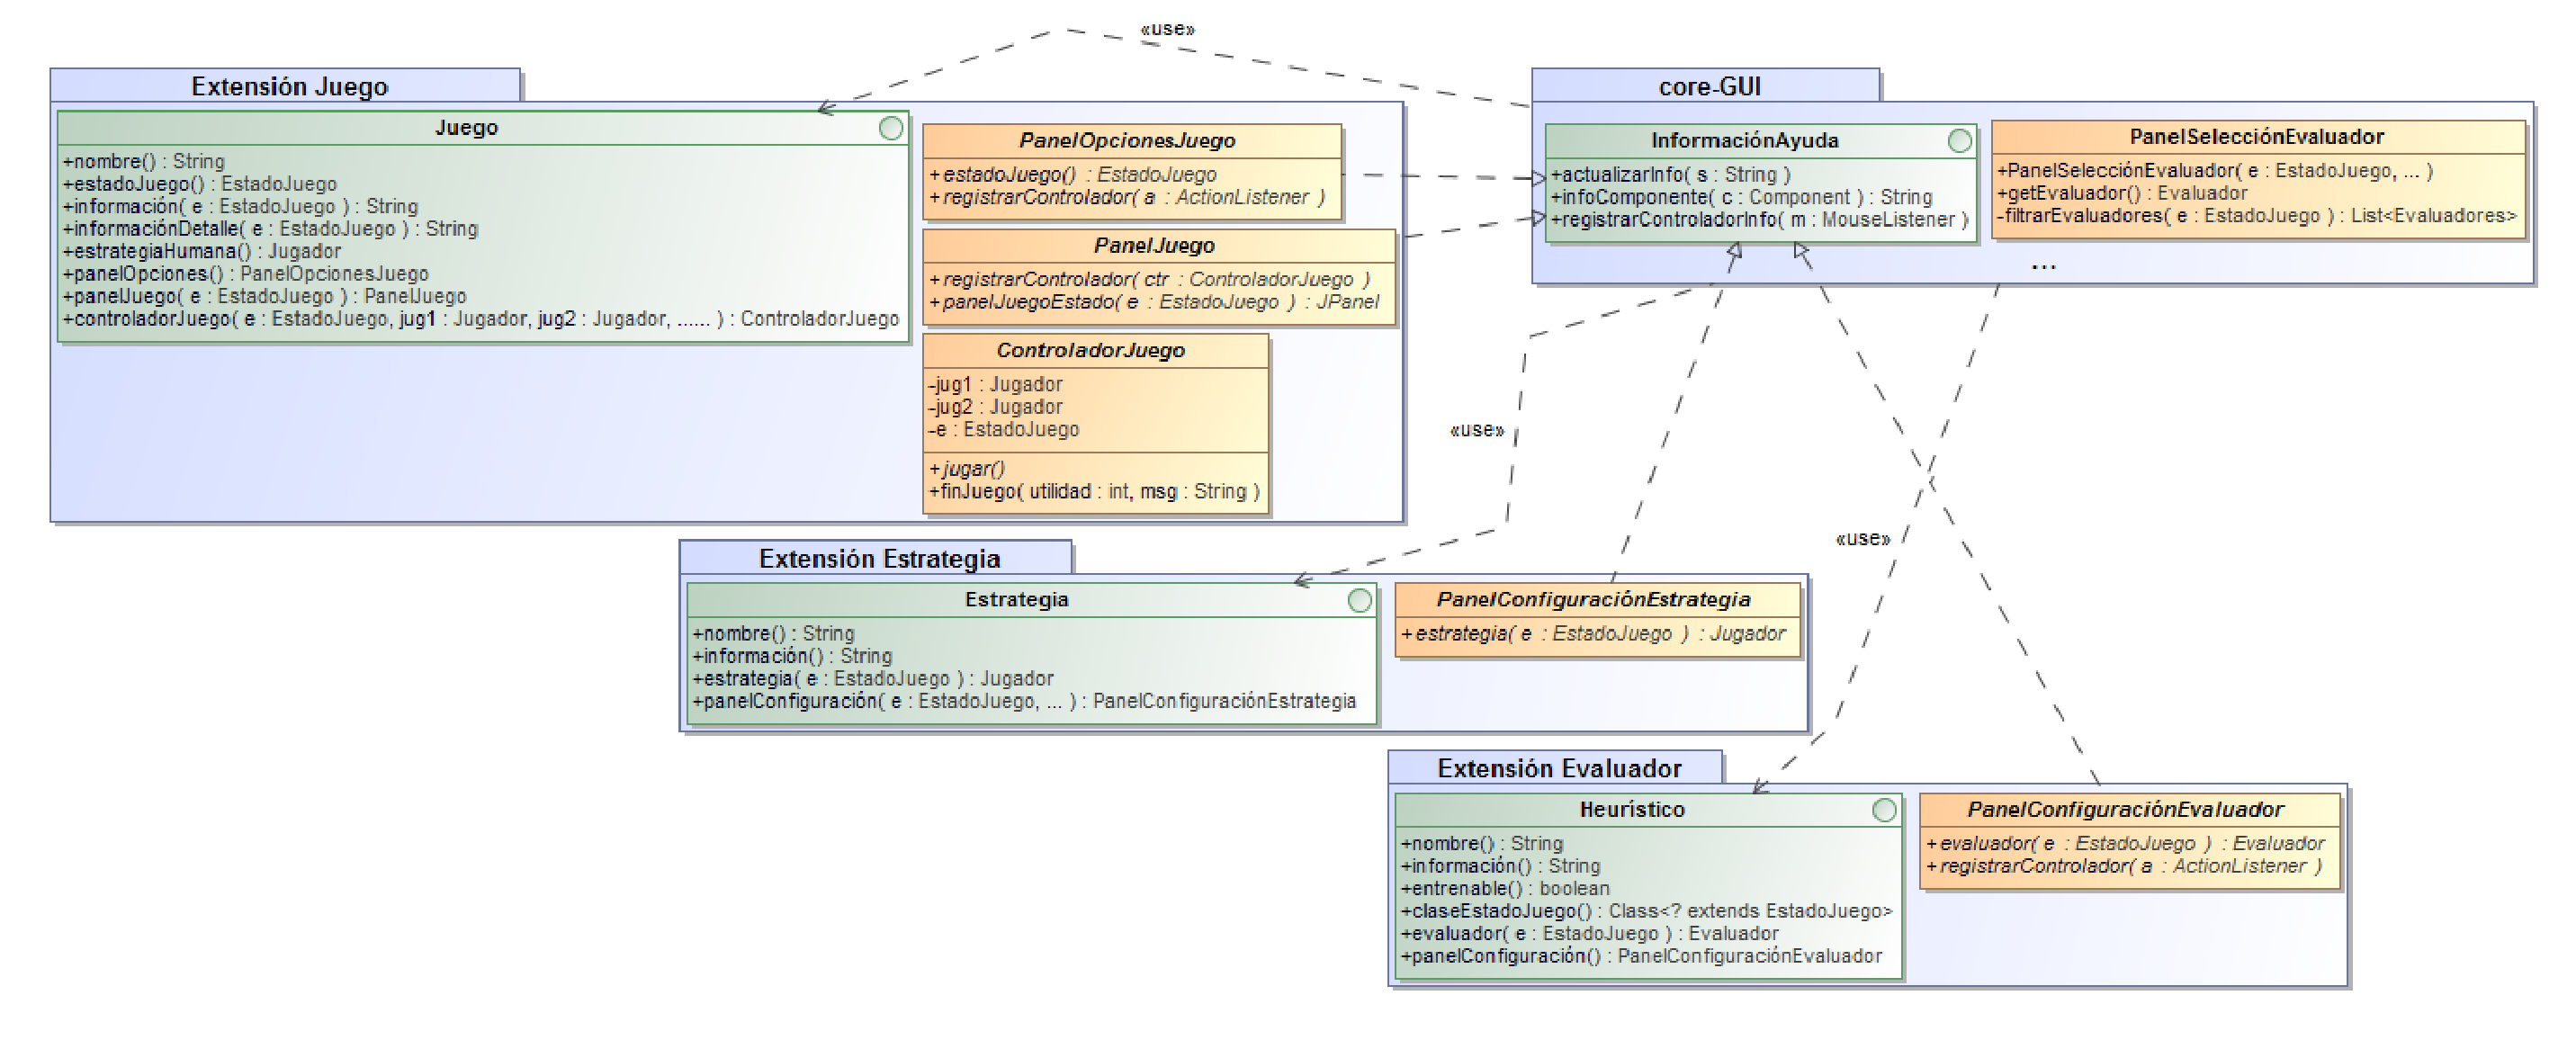
\includegraphics[scale=0.4,angle=90]{contenido/cap6/imagenes/diagramaclases_gui.eps}
	\caption{Diagrama de clases de las extensiones de la interfaz gráfica.}
	\label{fig:diagramaclases_gui}
\end{figure}

Todos los juegos, estrategias y heurísticos desarrollados se han incorporado a la interfaz de la aplicación interactiva siguiendo el esquema mostrado.
Cada elemento debe implementar su respectiva interfaz, lo que supone a su vez desarrollar los paneles de configuración adecuados, los controladores o el tablero para los juegos.

El núcleo de la interfaz gráfica consta de las vistas y los controladores necesarios para llevar a cabo los casos de uso de la aplicación, aunque estas clases no se muestran en el diagrama.

El sistema de información de ayuda está representado por la interfaz \texttt{\textit{InformaciónAyuda}}, que es implementada por cada componente visual de la interfaz gráfica (pantallas y paneles) usando el patrón de diseño \textit{Cadena de Mando} (\textit{Chain of Responsability}).
El usuario puede obtener información de ayuda sobre cualquier parte de la interfaz situándose sobre ella; la ayuda que se obtiene depende de la parte de la interfaz sobre la que solicita y de su contexto.

Por último, destacar que la aplicación se ha realizado íntegramente sobre tecnología \textit{Java} \citeref{java} en su versión 1.6; aunque el diseño propuesto permite desarrollar el entorno interactivo al completo en cualquier lenguaje de programación orientado a objetos.
La documentación en este proyecto es un aspecto clave, por lo que todo el código desarrollado se encuentra documentado en formato \textit{javadoc} para que cualquier alumno, profesor o investigador pueda hacer uso de él.



% 6. Experimentación
\chapter{Experimentación}
\label{cap:experimentacion}
Este capítulo muestra algunas de las pruebas realizadas y los resultados obtenidos.
Se comparan diferentes estrategias en los dos juegos desarrollados.
Para ello se han realizado varias simulaciones y análisis de estados con las estrategias.

La siguiente sección se centra en las pruebas realizadas a los evaluadores heurísticos de cada juego, incluyendo algunas series de entrenamientos para los evaluadores entrenables.

\section{Comparativa de evaluadores heurísticos}  
\label{sec:comparativa_evaluadores_heuristicos}
Primero se han comparado los evaluadores heurísticos de cada uno de los juegos de forma independiente.

\subsection{Evaluadores del Conecta-4}
\label{ssec:comparativa_evaluadores_conecta4}
Para comparar los evaluadores heurísticos del Conecta-4 se han jugado 100 partidas entre un jugador evaluador (\texttt{JugadorEvaluar}) y un jugador aleatorio para cada prueba.
Recordemos que un \texttt{JugadorEvaluar} considera todos los movimientos inmediatos, los evalúa heurísticamente y escoge el mejor.

Las pruebas se han realizado en un tablero de dimensiones 6x7 con una longitud ganadora de cuatro fichas.
Los evaluadores heurísticos usados son la matriz de posibilidades (número de posibilidades de conectar cuatro fichas de \textit{MAX} menos el número de posibilidades de conectar cuatro fichas que tiene \textit{MIN}), la tabla de valor y la red neuronal.
La tabla de valor y la red neuronal se han entrenado con 2.000 partidas frente a un jugador aleatorio, con una tasa de aprendizaje de 0.1 y una tasa de exploración de 0.1.
La red neuronal cuenta con una única neurona en la capa intermedia.

Las tablas~\ref{tab:comparativa_heuristicos_conecta4_jug1} y \ref{tab:comparativa_heuristicos_conecta4_jug2} presentan los resultados de las pruebas realizadas con el \texttt{JugadorEvaluar} jugando como primer jugador y como segundo jugador respectivamente.
Las figuras~\ref{fig:comparativa_heuristicos_conecta4_jug1} y \ref{fig:comparativa_heuristicos_conecta4_jug2} muestran de forma gráfica estos resultados. 

% HEURISTICOS CONECTA-4
\begin{table}[!h]
\centering
\caption[Comparativa de los evaluadores heurísticos del Conecta-4 (I)]{Comparativa de los evaluadores heurísticos del Conecta-4 para el primer jugador.}
\label{tab:comparativa_heuristicos_conecta4_jug1}
\begin{tabular}{lccc}
\hline
\textbf{Jugador 1:} & \textbf{Ev. Heur. (Matriz de posibilidades)} & \textbf{Tabla de valor} & \textbf{Red neuronal} \\
%\hline
\textbf{Gana} & 98\% & 84\% & 88\% \\
\textbf{Empata} & 0\% & 0\% & 0\% \\
\textbf{Pierde} & 2\% & 16\% & 12\% \\
\hline
\end{tabular}
\end{table} 

\begin{figure}[!h]
	\centering
	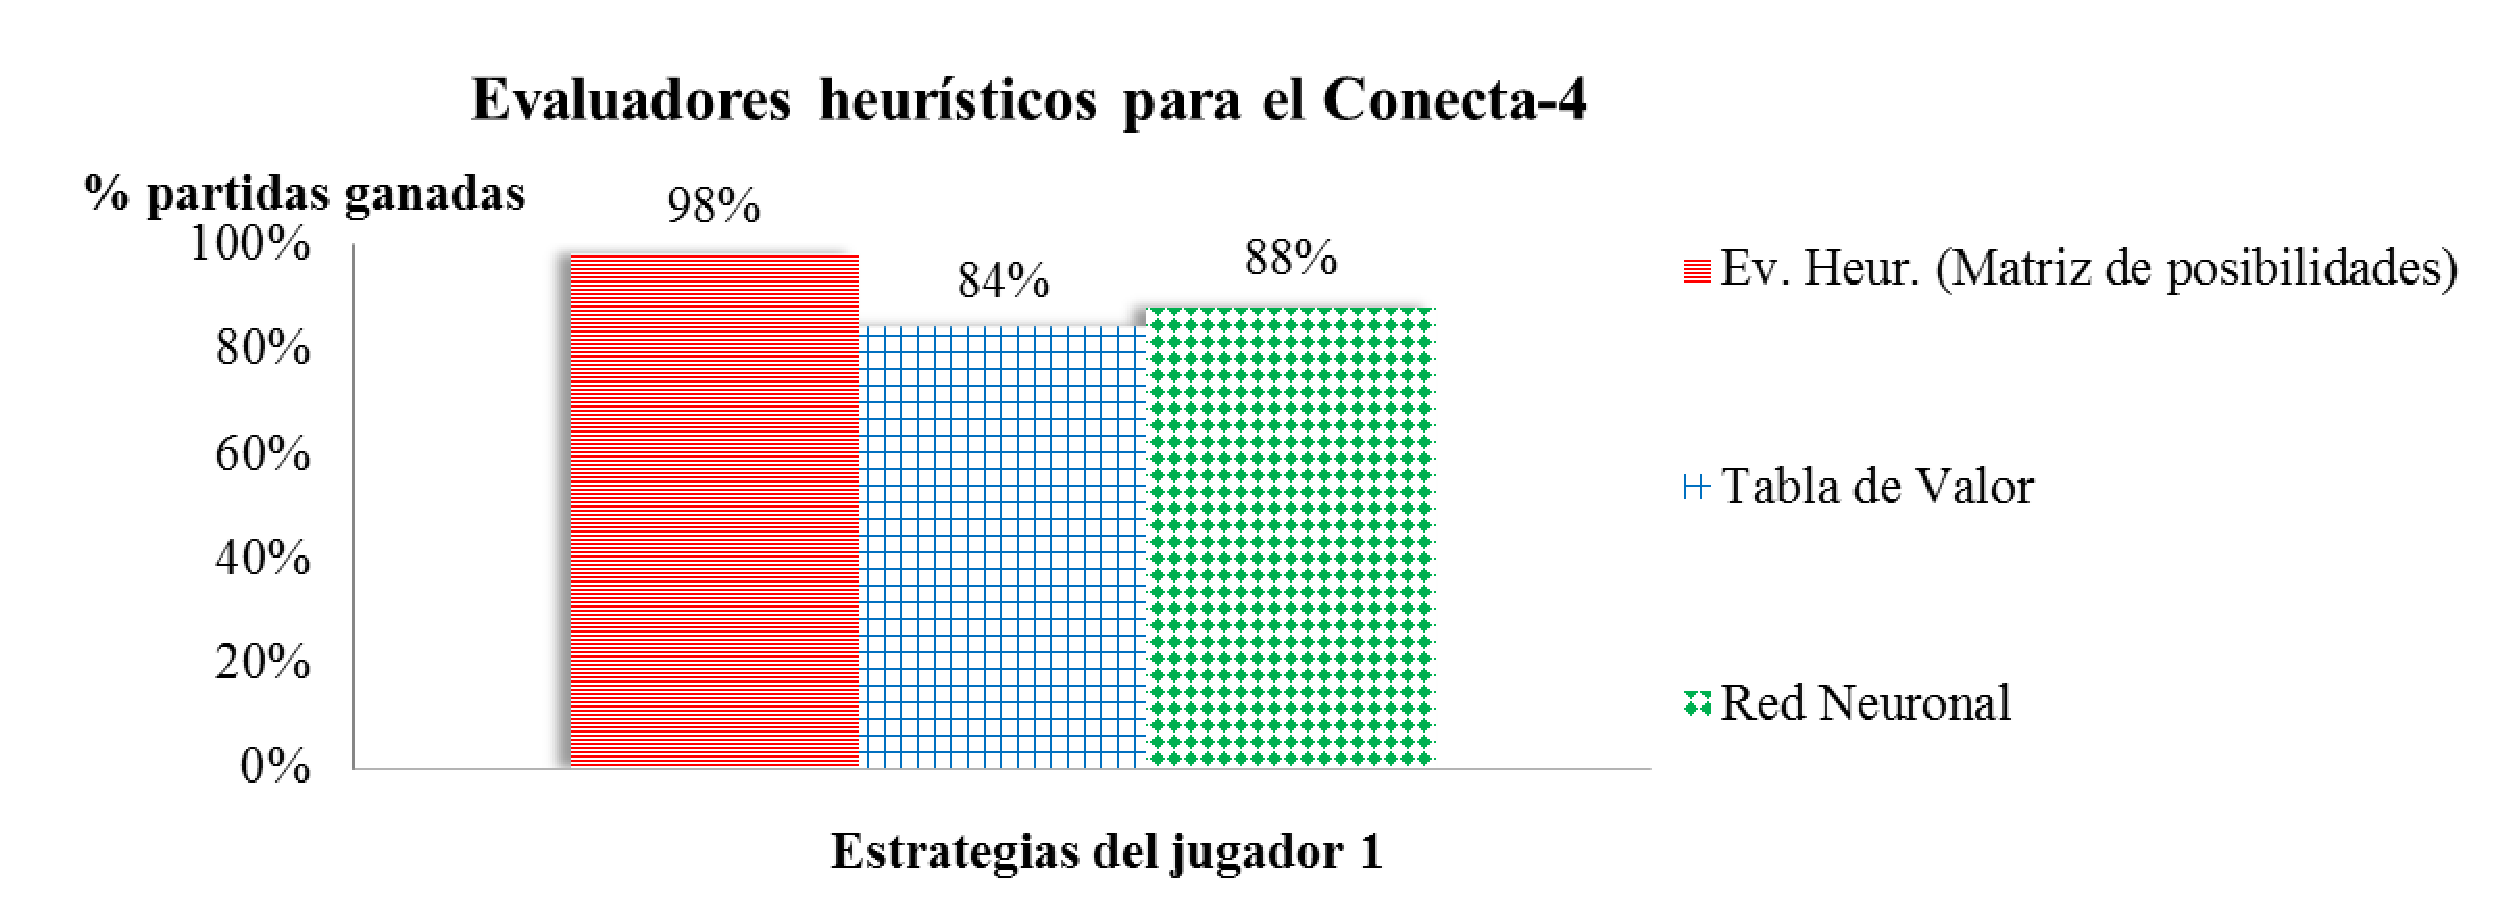
\includegraphics[scale=0.3]{contenido/cap7/imagenes/heuristicosConecta4jug1.eps}
	\caption[Comparativa de los evaluadores heurísticos del Conecta-4 (I)]{Gráfica comparativa de los evaluadores heurísticos del Conecta-4 para el primer jugador.}
	\label{fig:comparativa_heuristicos_conecta4_jug1}
\end{figure}

\begin{table}[!h]
\centering
\caption[Comparativa de los evaluadores heurísticos del Conecta-4 (II)]{Comparativa de los evaluadores heurísticos del Conecta-4 para el segundo jugador.}
\label{tab:comparativa_heuristicos_conecta4_jug2}
\begin{tabular}{lccc}
\hline
\textbf{Jugador 2:} & \textbf{Ev. Heur. (Matriz de posibilidades)} & \textbf{Tabla de valor} & \textbf{Red neuronal} \\
%\hline
\textbf{Gana} & 94\% & 78\% & 81\% \\
\textbf{Empata} & 0\% & 0\% & 1\% \\
\textbf{Pierde} & 6\% & 22\% & 18\% \\
\hline
\end{tabular}
\end{table} 

\begin{figure}[!h]
	\centering
	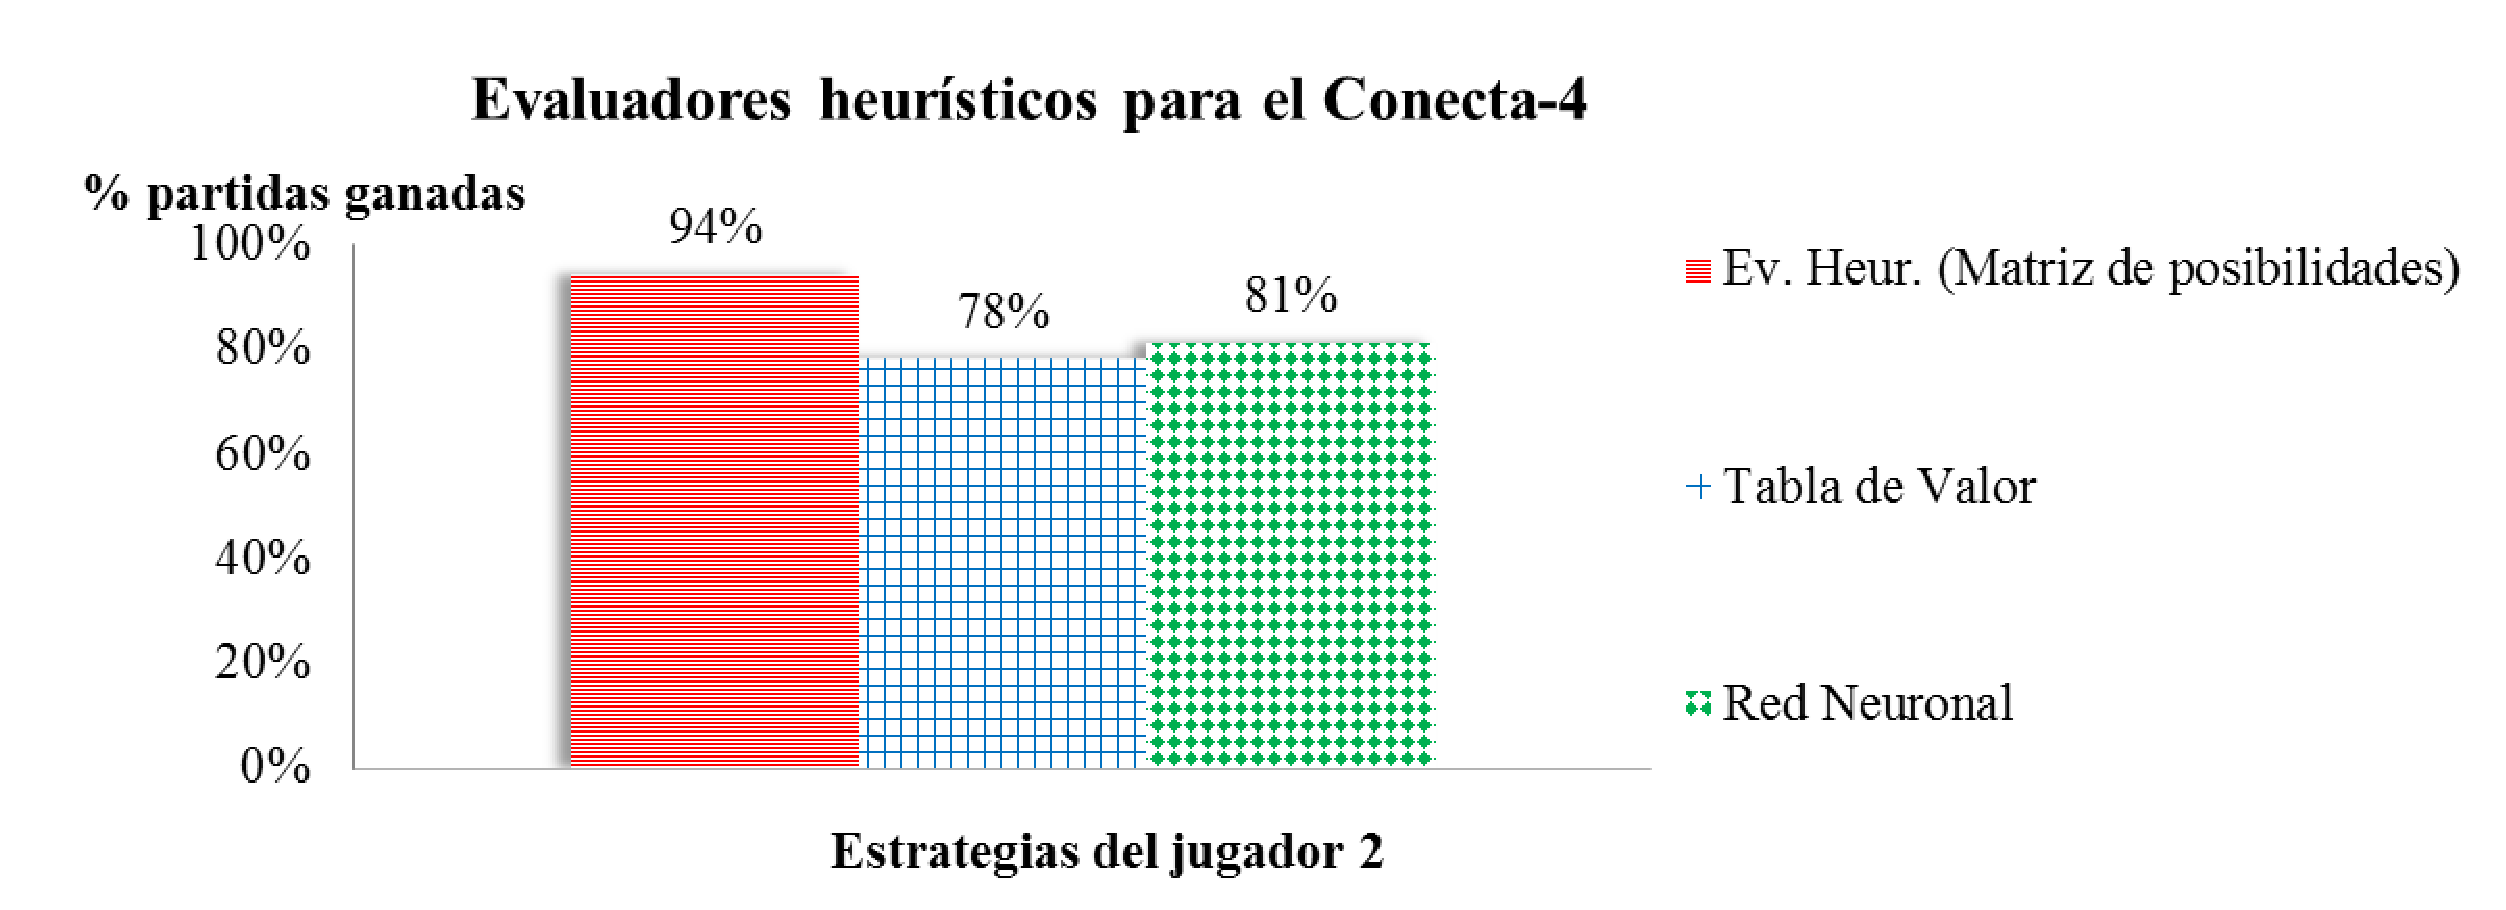
\includegraphics[scale=0.3]{contenido/cap7/imagenes/heuristicosConecta4jug2.eps}
	\caption[Comparativa de los evaluadores heurísticos del Conecta-4 (II)]{Gráfica comparativa de los evaluadores heurísticos del Conecta-4 para el segundo jugador.}
	\label{fig:comparativa_heuristicos_conecta4_jug2}
\end{figure} 
 
Se observa que un evaluador que utilice información de la situación actual del juego para realizar la evaluación ofrece mejores resultados que un evaluador que no tenga en cuenta esa información; aunque en este caso, con un número mayor de partidas de entrenamiento se pueden conseguir los mismos resultados.

\subsection{Evaluadores del Go}
\label{ssec:comparativa_evaluadores_go}
Para el juego del Go también también se han jugado 100 partidas entre un \texttt{JugadorEvaluar} y un jugador aleatorio para cada prueba.
Las pruebas se han realizado en un tablero de dimensiones 9x9, con las reglas de puntuación japonesas y sin puntos de ventaja para el segundo jugador.

Las tablas~\ref{tab:comparativa_heuristicos_go_jug1} y \ref{tab:comparativa_heuristicos_go_jug2} presentan los resultados de las pruebas para el juego del Go y las figuras~\ref{fig:comparativa_heuristicos_go_jug1} y \ref{fig:comparativa_heuristicos_go_jug2} muestran de forma gráfica los resultados. 
Los evaluadores heurísticos usados han sido un evaluador basado en el número de territorios (Territorios), uno basado en los puntos según las reglas chinas (P. CH), otro basado en los puntos según las reglas japonesas (P. JP), la tabla de valor y la red neuronal.
La tabla de valor y la red neuronal se han entrenado con 2.000 partidas frente a un jugador aleatorio, con los mismos parámetros de entrenamiento que en el experimento anterior.
La red neuronal cuenta con nueve neuronas en la capa intermedia.

% HEURISTICOS GO
\begin{table}[!h]
\centering
\caption[Comparativa de los evaluadores heurísticos del Go (I)]{Comparativa de los evaluadores heurísticos del Go para el primer jugador.}
\label{tab:comparativa_heuristicos_go_jug1}
\begin{tabular}{lccccc}
\hline
\textbf{Jugador 1:} & \textbf{Territorios} & \textbf{P. CH} & \textbf{P. JP} & \textbf{Tabla de valor} & \textbf{Red neuronal} \\
%\hline
\textbf{Gana} & 94\% & 100\% & 97\% & 72\% & 99\% \\
\textbf{Empata} & 0\% & 0\% & 0\% & 0\% & 0\% \\
\textbf{Pierde} & 6\% & 0\% & 3\% & 24\% & 1\% \\
\hline
\end{tabular}
\end{table} 

\begin{figure}[!h]
	\centering
	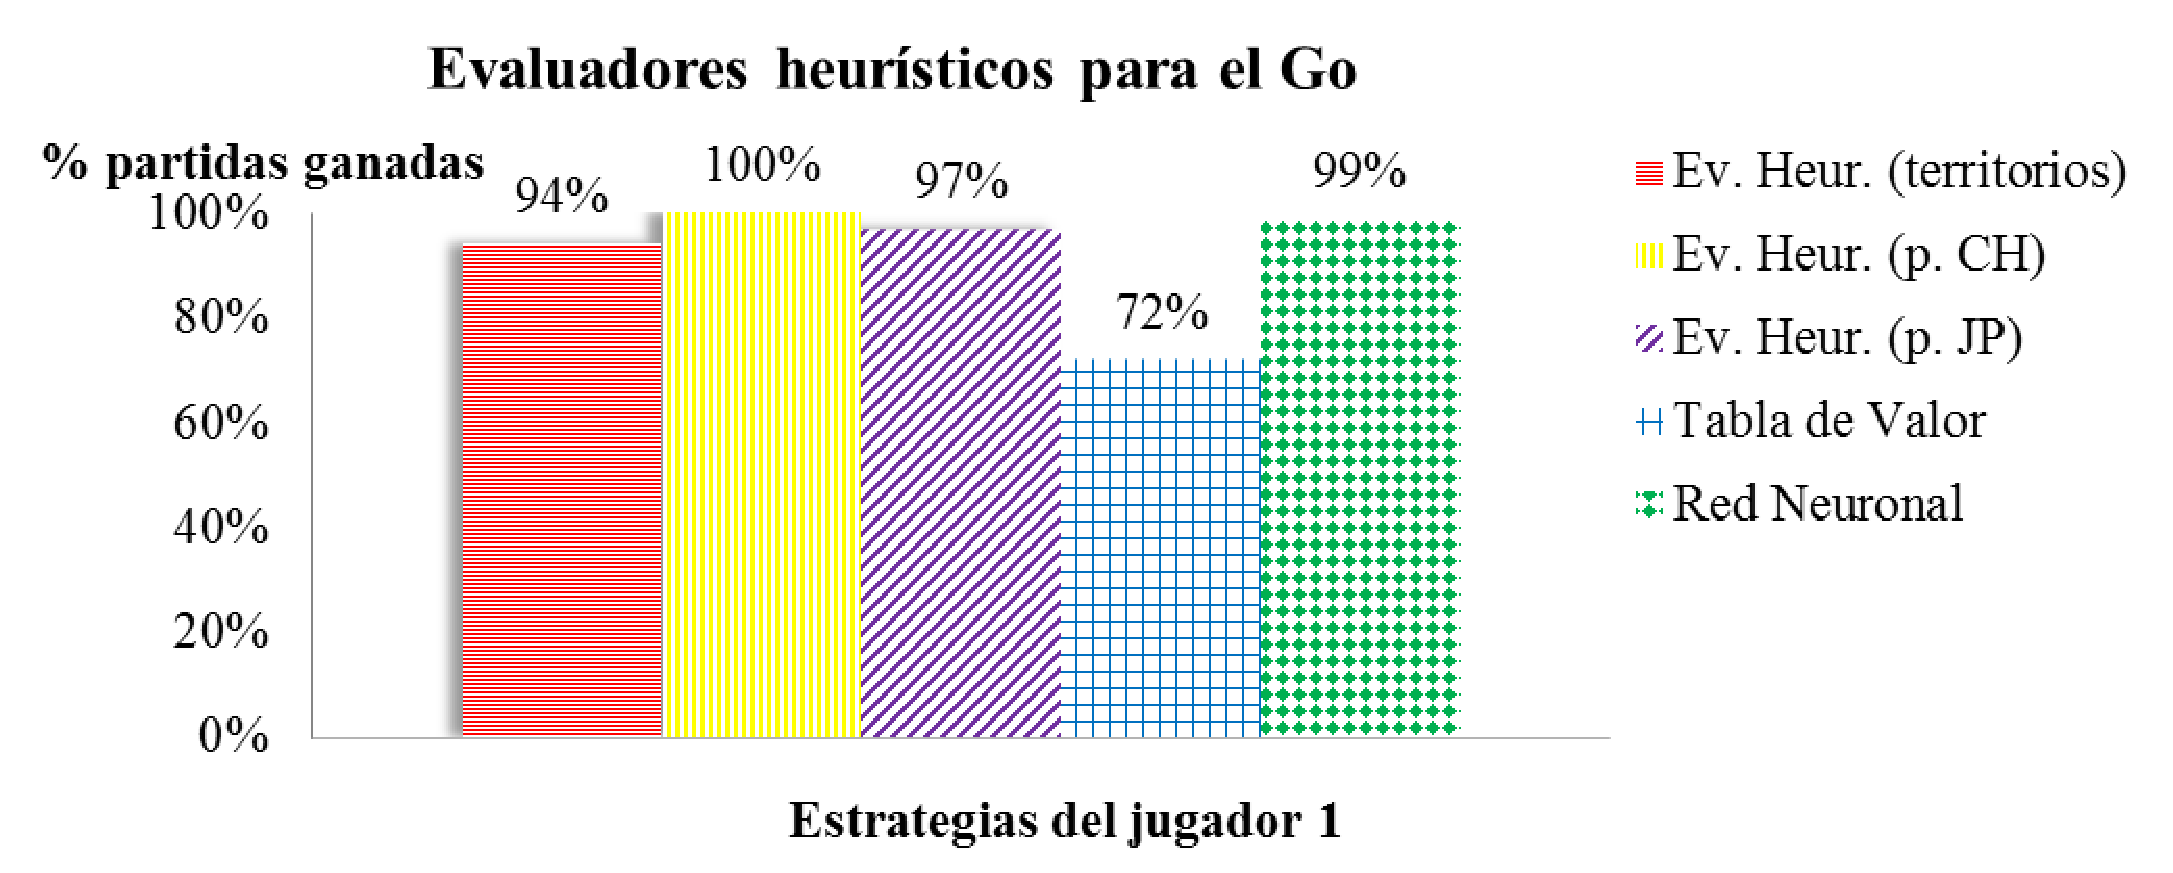
\includegraphics[scale=0.3]{contenido/cap7/imagenes/heuristicosGojug1.eps}
	\caption[Comparativa de los evaluadores heurísticos del Go (I)]{Gráfica comparativa de los evaluadores heurísticos del Go para el primer jugador.}
	\label{fig:comparativa_heuristicos_go_jug1}
\end{figure}

\begin{table}[b]
\centering
\caption[Comparativa de los evaluadores heurísticos del Go (II)]{Comparativa de los evaluadores heurísticos del Go para el segundo jugador.}
\label{tab:comparativa_heuristicos_go_jug2}
\begin{tabular}{lccccc}
\hline
\textbf{Jugador 2:} & \textbf{Territorios} & \textbf{P. CH} & \textbf{P. JP} & \textbf{Tabla de valor} & \textbf{Red neuronal} \\
%\hline
\textbf{Gana} & 93\% & 99\% & 95\% & 67\% & 65\% \\
\textbf{Empata} & 0\% & 0\% & 0\% & 1\% & 2\% \\
\textbf{Pierde} & 7\% & 1\% & 5\% & 32\% & 33\% \\
\hline
\end{tabular}
\end{table} 

\begin{figure}[!h]
	\centering
	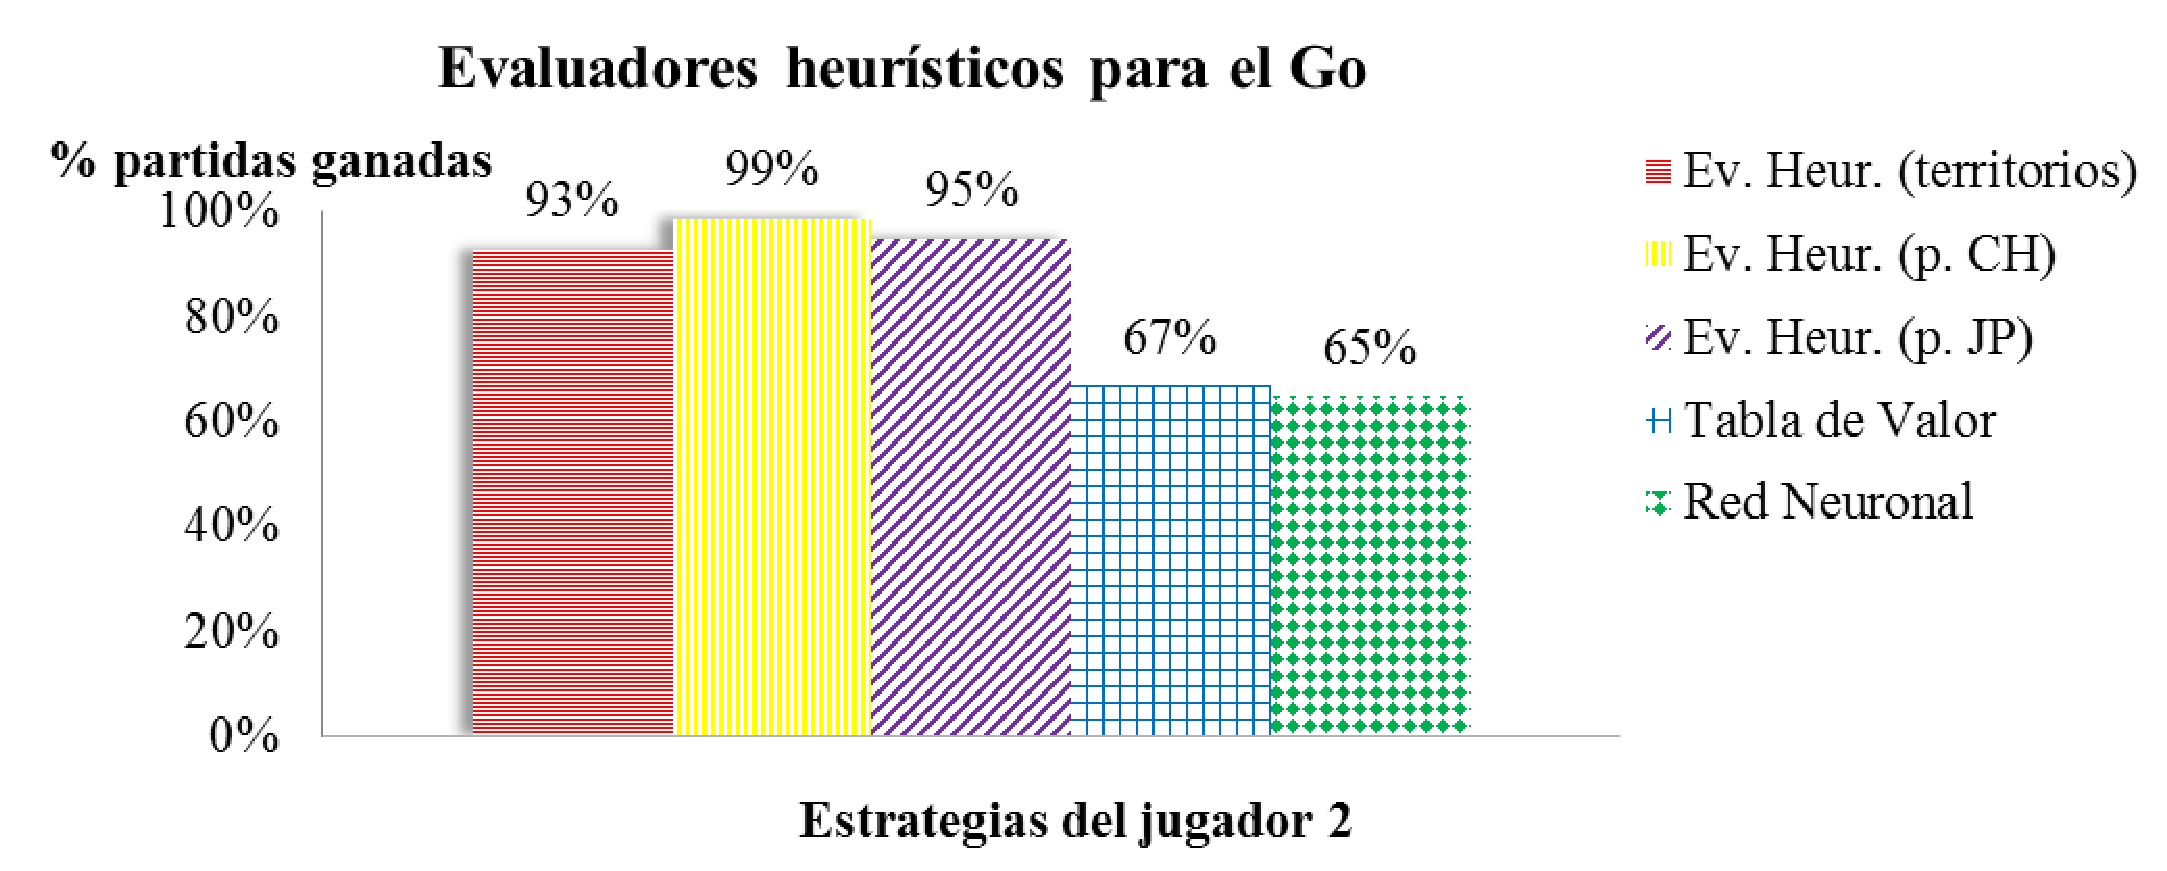
\includegraphics[scale=0.3]{contenido/cap7/imagenes/heuristicosGojug2.eps}
	\caption[Comparativa de los evaluadores heurísticos del Go (II)]{Gráfica comparativa de los evaluadores heurísticos del Go para el segundo jugador.}
	\label{fig:comparativa_heuristicos_go_jug2}
\end{figure} 

En el caso del Go la diferencia entre los evaluadores que usan información del dominio y los que no es más evidente, sobre todo para el segundo jugador; esto se debe a que el tamaño del espacio de estados del Go es mayor que el del Conecta-4, lo que además hace que una estrategia aleatoria sea muy fácil de vencer.
Los evaluadores entrenables también necesitan más partidas de entrenamiento para conseguir los mismos resultados que el resto de evaluadores.

\subsection{Entrenamientos}
\label{ssec:comparativa_entrenamientos}
En esta sección se estudian varias secuencias de entrenamiento en el juego del Go.
Se ha considerado un tablero 9x9 con las reglas de puntuación japonesas y sin ninguna ventaja para el segundo jugador.

Se entrenan cuatro jugadores diferentes con red neuronal (\texttt{JugadorEvaluar}): uno como primer jugador frente a una estrategia aleatoria (J1), otro como segundo jugador frente a una estrategia aleatoria (J2) y los otros dos jugadores se entrenan simultáneamente uno frente al otro (J3 y J4).
En todos los casos la red neuronal dispone de nueve neuronas en la capa intermedia y los pesos iniciales son aleatorios, la tasa de aprendizaje para ajustar la velocidad a la que aprende la red tiene un valor de 0.1 y el momento de entrenamiento que indica la influencia que tiene la iteración anterior sobre la actual es de 0.8.

Las tablas~\ref{tab:secuencia1}, \ref{tab:secuencia2} y \ref{tab:secuencia2} muestran cómo evoluciona el aprendizaje de la red neuronal para cada uno de los casos.
Las tres secuencias de entrenamiento constan de 2.000 partidas, mostrándose cada 100 los resultados de 100 partidas sin aprendizaje.
En todos los casos se toman las últimas redes, es decir, las obtenidas después de los entrenamiento completos de 2.000 partidas, independientemente de los resultados obtenidos durante el proceso.
Esto puede dar lugar a un sobreaprendizaje, como se observa en la secuencia 3.

Las figuras~\ref{fig:secuencia1}, \ref{fig:secuencia2} y \ref{fig:secuencia3} muestran de forma gráfica la evolución del aprendizaje para cada secuencia de entrenamiento.

\begin{table}[t]
	\centering
	% Primera imagen
	\begin{minipage}[t]{0.4\linewidth}
		\centering
		\caption[Secuencia de entrenamiento 1]{Secuencia 1.}
		\label{tab:secuencia1}
				{\footnotesize
				\begin{tabular}{rrrr}
\hline
\textbf{Nº partidas} & \textbf{J1} & \textbf{Empate} & \textbf{Aleatorio} \\
%\hline
0	& 42\% &	4\%	& 54\% \\
100	& 41\% &	3\%	& 56\% \\
200	& 24\% &	8\%	& 68\% \\
300	& 37\% &	3\%	& 60\% \\
400	& 21\% &	5\%	& 74\% \\
500	& 25\% &	4\%	& 71\% \\
600	& 63\% &	3\%	& 34\% \\
700	& 67\% &	1\%	& 32\% \\
800	& 43\% &	3\%	& 54\% \\
900	& 61\% &	0\%	& 39\% \\
1000 &	57\% &	0\%	& 43\% \\
1100 &	87\% &	0\%	& 13\% \\
1200 &	87\% &	0\%	& 13\% \\
1300 &	73\% &	0\%	& 27\% \\
1400 &	94\% &	0\%	& 6\% \\
1500 &	99\% &	0\%	& 1\% \\
1600 &	98\% &	0\%	& 2\% \\
1700 &	97\% &	0\%	& 3\% \\
1800 &	98\% &	0\%	& 2\% \\
1900 &	98\% &	0\%	& 2\% \\
2000 &	96\% &	0\%	& 4\% \\
\hline
\end{tabular}
}
	\end{minipage}
	\hspace{1cm}
	% Segunda imagen
	\begin{minipage}[t]{0.4\linewidth}
		\centering
		\caption[Secuencia de entrenamiento 2]{Secuencia 2.}
		\label{tab:secuencia2}
			{\footnotesize
				\begin{tabular}{rrrr}
\hline
\textbf{Nº partidas} & \textbf{Aleatorio} & \textbf{Empate} & \textbf{J2} \\
%\hline
0	& 50\% &	0\% &	48\% \\
100	& 35\% &	0\% &	61\% \\
200	& 43\% &	0\% &	51\% \\
300	& 53\% &	0\% &	45\% \\
400	& 37\% &	0\% &	61\% \\
500	& 35\% &	0\% &	65\% \\
600	& 49\% &	0\% &	51\% \\
700	& 51\% &	0\% &	47\% \\
800	& 8\% &	0\%	 &92\% \\
900	& 6\% &	0\%	 &94\% \\
1000 &	14\% &	0\%	 & 85\% \\
1100 &	17\% &	0\%	 & 82\% \\
1200 &	33\% &	0\%	 & 65\% \\
1300 &	15\% &	0\% &	85\% \\
1400 &	11\% &	0\% &	89\% \\
1500 &	15\% &	0\% &	85\% \\
1600 &	12\% &	0\% &	88\% \\
1700 &	18\% &	0\% &	82\% \\
1800 &	16\% &	0\% &	84\% \\
1900 &	7\%	&   0\%	 & 93\% \\
2000 &	33\% &	0\% &	67\% \\
\hline
\end{tabular}
}
	\end{minipage}
\end{table}

\begin{table}[t]
\caption[Secuencia de entrenamiento 3]{Secuencia 3.}
\label{tab:secuencia3}
\centering
{\footnotesize
\begin{tabular}{rrrr}
\hline
\textbf{Nº partidas} & \textbf{Aleatorio} & \textbf{Empate} & \textbf{J2} \\
%\hline
0	& 0\% &	0\% &	100\% \\
100	&0\% &	0\% &	100\% \\
200	&0\% &	0\% &	100\% \\
300	&100\% &	0\% &	0\% \\
400	&100\% &	0\% &	0\% \\
500	&100\% &	0\% &	0\% \\
600	&100\% &	0\% &	0\% \\
700	&100\% &	0\% &	0\% \\
800	&0\% &	0\% &	100\% \\
900	&100\% &	0\% &	0\% \\
1000 &	0\% &	0\% &	100\% \\
1100 &	100\% &	0\% &	0\% \\
1200 &	0\% &	0\% &	100\% \\
1300 &	0\% &	100\% &	0\% \\
1400 &	0\% &	100\% &	0\% \\
1500 &	0\% &	100\% &	0\% \\
1600 &	0\% &	100\% &	0\% \\
1700 &	100\% &	0\% &	0\% \\
1800 &	0\% &	100\% &	0\% \\
1900 &	100\% &	0\% &	0\% \\
2000 &	100\% &	0\% &	0\% \\
\hline
\end{tabular}
}
\end{table} 

En el aprendizaje pueden presentarse oscilaciones, por lo que puede ser necesario cierto grado de experimentación antes de obtener una red correctamente entrenada.

Los valores de la secuencia número 3 pueden parecer extraños, esto se debe a que la red neuronal siempre devuelve el mismo movimiento para un estado dado y por lo tanto siempre se juegan las mismas partidas entre las dos redes neuronales; sin embargo, es más provechoso entrenar a dos jugadores simultáneamente (cada uno aprendiendo de su juego con el otro) que usando un jugador aleatorio.
A medida que se aumenta el tamaño del tablero de juego, el jugador aleatorio es menos eficaz para entrenar a los jugadores.

\begin{figure}[t]
	\centering
	% Primera imagen
	\begin{minipage}[t]{0.4\linewidth}
		\centering
		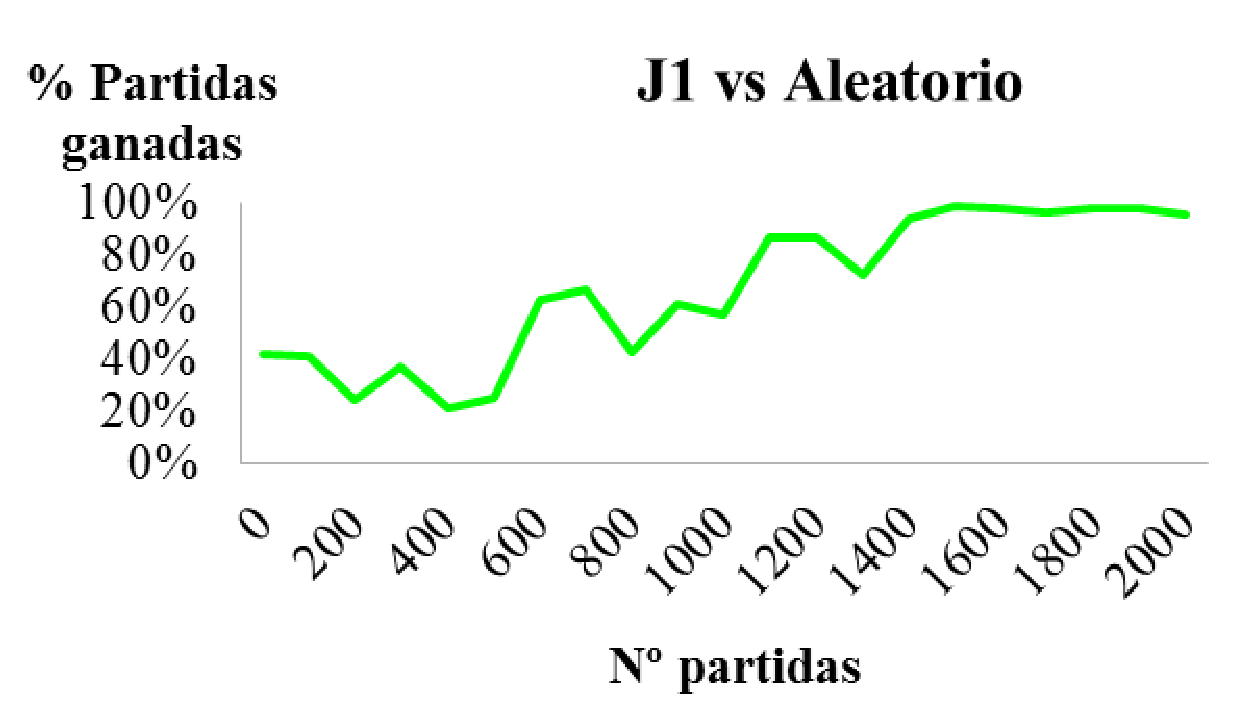
\includegraphics[scale=0.3]{contenido/cap7/imagenes/entrenamientoSecuencia1.eps}
		\caption[Secuencia de entrenamiento 1]{Secuencia 1.}
		\label{fig:secuencia1}
	\end{minipage}
	\hspace{1cm}
	% Segunda imagen
	\begin{minipage}[t]{0.4\linewidth}
		\centering
		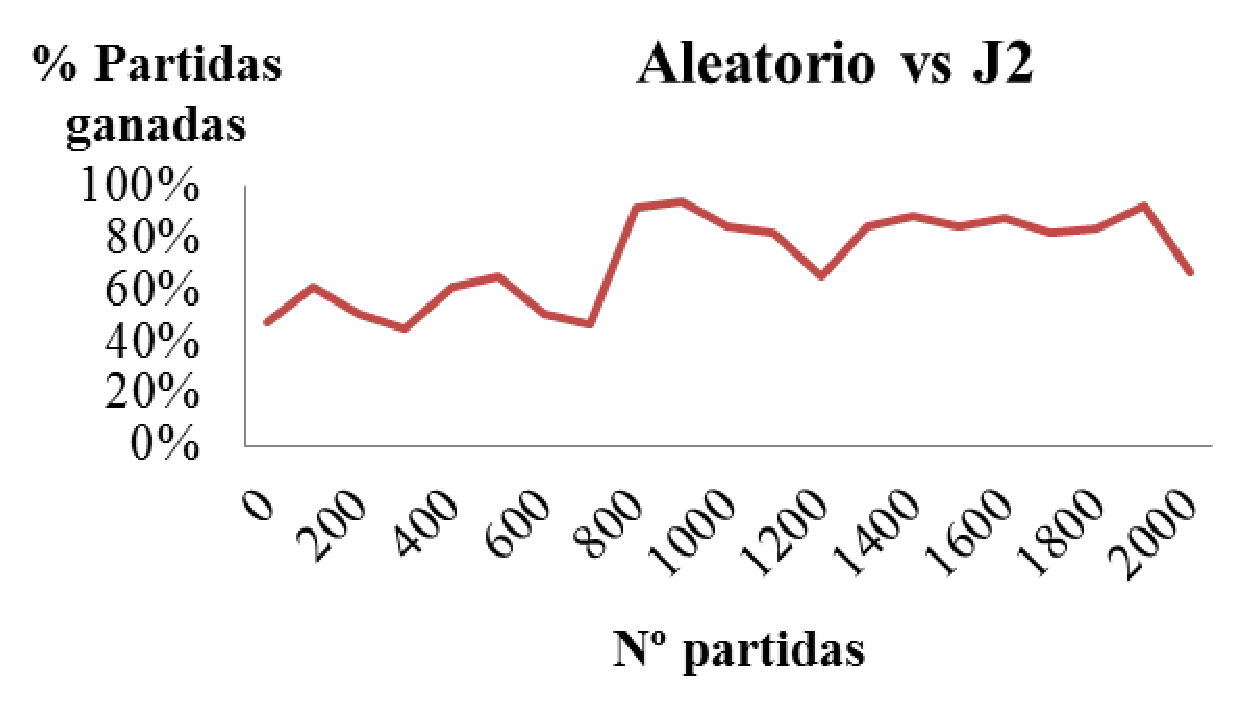
\includegraphics[scale=0.3]{contenido/cap7/imagenes/entrenamientoSecuencia2.eps}
		\caption[Secuencia de entrenamiento 2]{Secuencia 2.}
		\label{fig:secuencia2}
	\end{minipage}
\end{figure}

\begin{figure}[t]
	\centering
	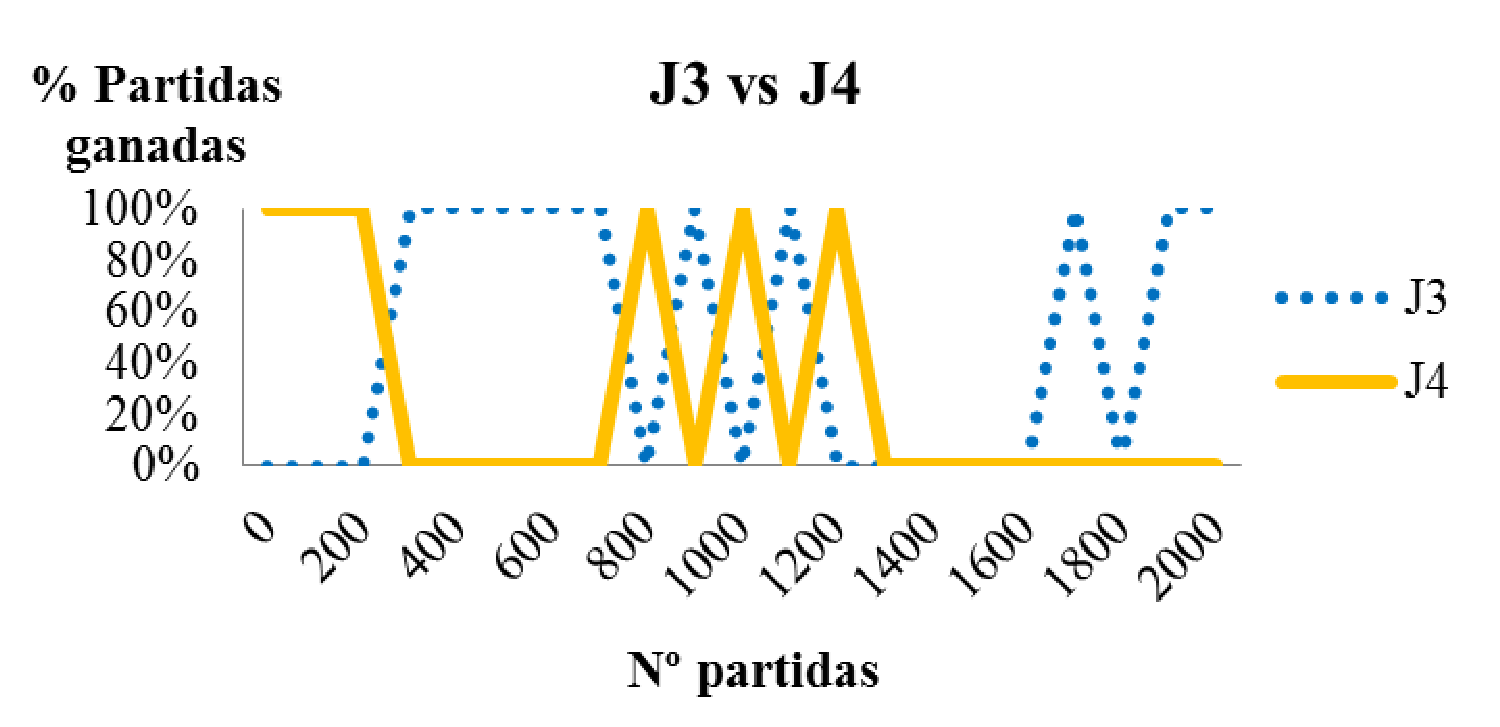
\includegraphics[scale=0.3]{contenido/cap7/imagenes/entrenamientoSecuencia3.eps}
	\caption[Secuencia de entrenamiento 3]{Secuencia 3.}
	\label{fig:secuencia3}
\end{figure} 

Con los jugadores entrenados, cada uno jugará 100 partidas frente a una estrategia aleatoria para comparar los resultados de los entrenamientos.
La tabla~\ref{tab:comparativa_resultados_entrenamientos} y la figura~\ref{fig:comparativa_resultados_entrenamientos} presentan los resultados de estas pruebas.
Se observa que en el caso del jugador J4 se han obtenido mejores resultados que para el jugador J2.
Recordemos que J4 entrena frente a otro jugador que aprende simultáneamente (J3), mientras J2 entrena frente a un jugador aleatorio.

\begin{table}[t]
\centering
\caption{Resultados frente a una estrategia aleatoria.}
\label{tab:comparativa_resultados_entrenamientos}
\begin{tabular}{lcccc}
\hline
\textbf{Jugador 1:} & \textbf{J1} & \textbf{Aleatorio} & \textbf{J3} & \textbf{Aleatorio} \\
\textbf{Jugador 2:} & \textbf{Aleatorio} & \textbf{J2} & \textbf{Aleatorio} & \textbf{J4} \\
%\hline
\textbf{Gana jugador 1} & 99\% & 33\% & 78\% & 7\% \\
\textbf{Empate} & 0\% & 2\% & 3\% & 1\% \\
\textbf{Gana jugador 2}  & 1\% & 65\% & 19\% & 92\% \\
\hline
\end{tabular}
\end{table} 

\begin{figure}[t]
	\centering
	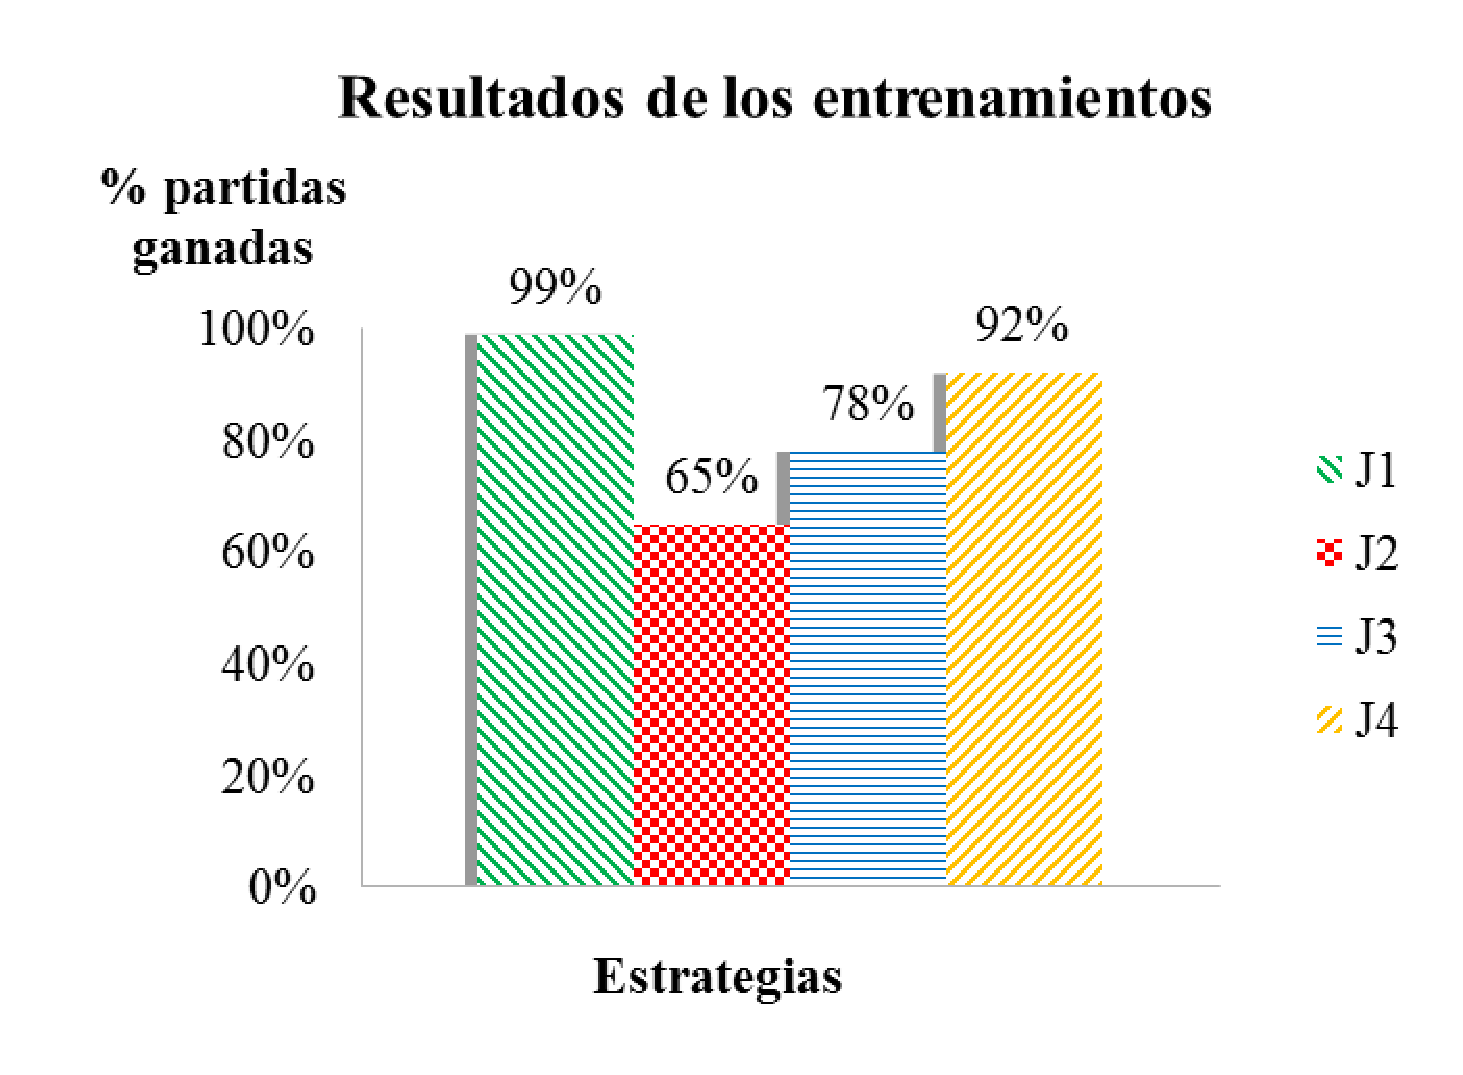
\includegraphics[scale=0.3]{contenido/cap7/imagenes/entrenamientosResultados.eps}
	\caption{Resultados de los entrenamientos.}
	\label{fig:comparativa_resultados_entrenamientos}
\end{figure} 

%\clearpage	% le dice a Latex que suelte todas las figuras en una página y comience una página nueva (detallado en los apuntes de los indios).

\section{Comparativa de estrategias}  
\label{sec:comparativa_estrategias}
En este sección se comparan algunas de las estrategias desarrolladas; para ello se analizan varios estados de los juegos y se realizan algunas simulaciones.

En primer lugar se compara la estrategia minimax frente a su versión mejorada con poda alfa-beta.
También se comparan las dos versiones desarrolladas del método de Monte-Carlo.
En estos casos se usará el juego del Conecta-4.
Por último se realizan varias pruebas en forma de simulaciones, donde cada estrategia juega frente a un jugador aleatorio en el juego del Go.

\subsection{Minimax y Alfa-Beta}
\label{ssec:comparativa_minimaxVSalfabeta}
A continuación se compara la eficacia de un jugador con poda alfa-beta frente a un jugador con el algoritmo minimax en su versión simple.
Se estudian dos estados del juego del Conecta-4 en un tablero 6x7: un estado inicial del juego y un estado intermedio en el que ya se han realizado varios movimientos.

\bigskip
Dado el estado inicial del juego del Conecta-4 (figura~\ref{fig:comparativa_minimax_alfabeta1}) se realiza una búsqueda en el árbol de juegos mediante las estrategias minimax y alfa-beta para obtener el mejor movimiento.
En ambos casos se limita la profundidad máxima de búsqueda al nivel 7.

\begin{figure}[b]
	\centering
	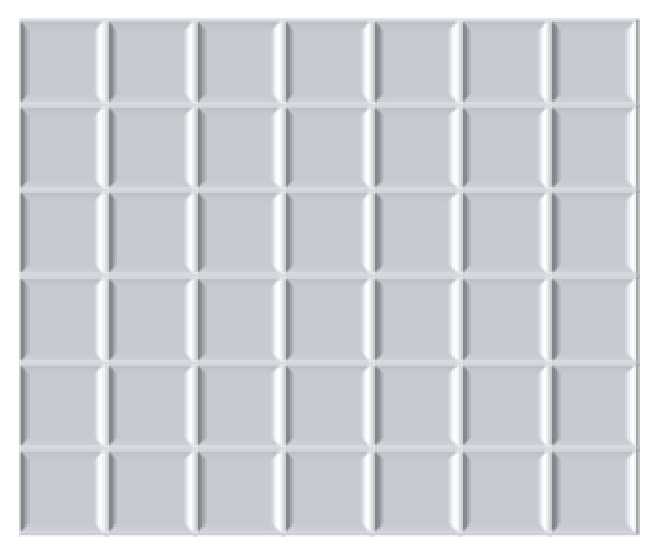
\includegraphics[scale=0.4]{contenido/cap7/imagenes/ckEstadoInicial.eps}
	\caption{Estado inicial del Conecta-4.}
	\label{fig:comparativa_minimax_alfabeta1}
\end{figure} 

En la tabla~\ref{tab:comparativa_minimax_alfabeta1} se muestran las estadísticas sobre la búsqueda del mejor movimiento posible.
Para cada nivel (desde 0 hasta la profundidad máxima) se muestra el número de nodos examinados en ese nivel por cada estrategia.
También se muestra el tiempo empleado en realizar la búsqueda.

\begin{table}[b]
\centering
\caption{Estadísticas de las estrategias minimax y alfa-beta.}
\label{tab:comparativa_minimax_alfabeta1}
\begin{tabular}{c|l|l}
\hline
& \multicolumn{1}{c|}{\textbf{Minimax}} & \multicolumn{1}{c}{\textbf{Alfa-Beta}}\\
\textbf{Profundidad} & \textbf{Nº nodos examinados} & \textbf{Nº nodos examinados} \\
%\hline
0 & 1 & 1 \\
1 & 7 & 7 \\
2 & 49 & 27 \\ 
3 & 343 & 118 \\
4 & 2.401 & 427 \\
5 & 16.807 & 1.621 \\
6 & 117.649 & 5.908 \\
7 & 823.536 & 22.103 \\
\hline
\textbf{Total:} & 960.793 nodos & 30.212 nodos \\
\textbf{Tiempo:} & 12,32 segundos & 1,10 segundos \\
\hline
\end{tabular}
\end{table} 

El mejor movimiento devuelto por ambas estrategias se muestra en la figura~\ref{fig:comparativa_minimax_alfabeta1Movimiento}, que corresponde a soltar una ficha en la columna central; obviamente tanto minimax como alfa-beta devuelven el mismo movimiento.
Se observa el importante ahorro de tiempo usando la poda alfa-beta; en algunos casos se llegan a podar ramas completas del árbol de juegos.

\begin{figure}[t]
	\centering
	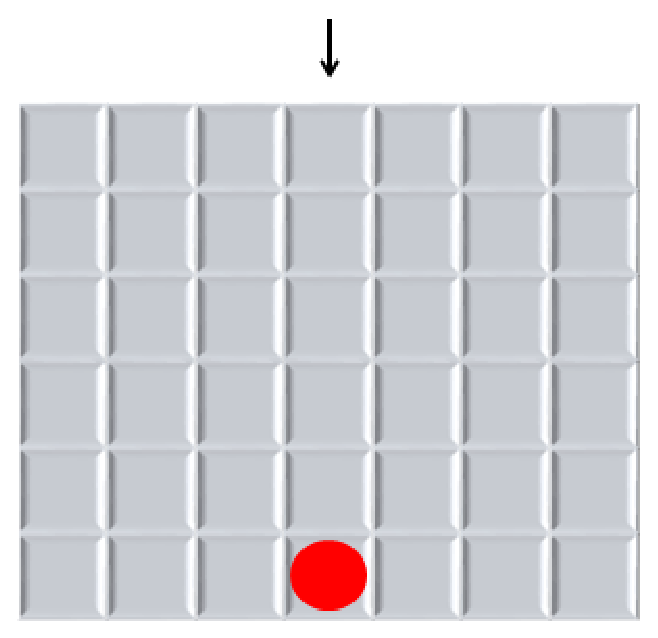
\includegraphics[scale=0.4]{contenido/cap7/imagenes/ckEstadoInicialMovimiento.eps}
	\caption[Mejor movimiento de minimax y alfa-beta en el Conecta-4 (I)]{Mejor movimiento devuelto por las estrategias minimax y alfa-beta para el estado inicial del Conecta-4.}
	\label{fig:comparativa_minimax_alfabeta1Movimiento}
\end{figure} 

\bigskip
En el siguiente ejemplo se considera un tablero ya inicializado correspondiente al estado mostrado en la figura~\ref{fig:comparativa_minimax_alfabeta2}. 
Le toca mover al primer jugador (\textit{MAX}) que juega con \textit{O}.
En este caso las estrategias minimax y alfa-beta disponen de un límite de tiempo de un segundo para realizar la búsqueda del mejor movimiento.

\begin{figure}[!h]
	\centering
	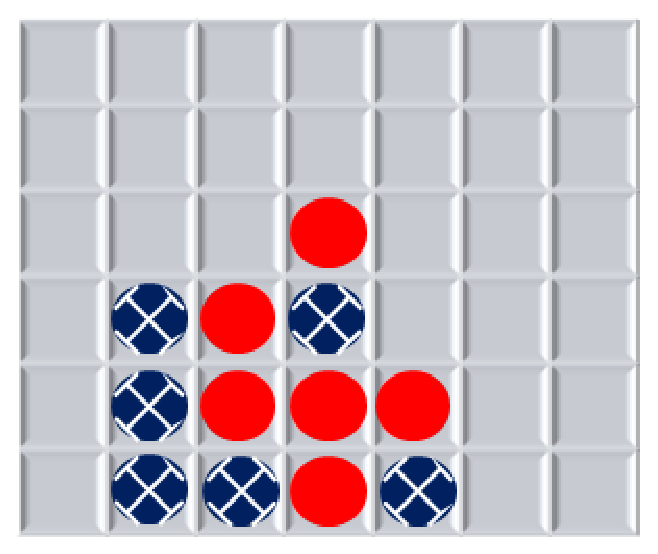
\includegraphics[scale=0.4]{contenido/cap7/imagenes/ckEstadoActual.eps}
	\caption{Estado inicializado del Conecta-4.}
	\label{fig:comparativa_minimax_alfabeta2}
\end{figure} 

La tabla~\ref{tab:comparativa_minimax_alfabeta2} presenta las estadísticas obtenidas en esta prueba.
Se muestra el número de nodos expandidos en cada iteración, teniendo en cuenta que las estrategias realizan una profundización progresiva.

\begin{table}[!h]
\centering
\caption[Estadísticas de minimax y alfa-beta con límite de tiempo]{Estadísticas de las estrategias minimax y alfa-beta con límite de tiempo.}
\label{tab:comparativa_minimax_alfabeta2}
\begin{tabular}{c|l|l}
\hline
& \multicolumn{1}{c|}{\textbf{Minimax}} & \multicolumn{1}{c}{\textbf{Alfa-Beta}}\\
\textbf{Iteración} & \textbf{Nº nodos expandidos} & \textbf{Nº nodos expandidos} \\
%\hline
0 & 1 & 1 \\
1 & 8 & 8 \\
2 & 57 & 37 \\ 
3 & 357 & 131 \\
4 & 2326 & 607 \\
5 & 14492 & 1721 \\
6 & 66420 & 2184 \\
7 &  & 13909 \\
8 &  & 57439 \\
\hline
\textbf{Total:} & 83661 nodos & 76037 nodos\\
\hline
\end{tabular}
\end{table} 

Mientras que minimax alcanza una profundidad máxima de búsqueda de 6 niveles, alfa-beta consigue llegar hasta una profundidad de 8 niveles en el mismo tiempo.
El número de nodos expandidos con la estrategia alfa-beta es sólo orientativo pues en cada profundización pueden expandirse más o menos nodos dependiendo de si se producen o no podas.


La figura~\ref{fig:comparativa_minimax_alfabeta2Movimiento} muestra el mejor movimiento devuelto por las dos estrategias, que en este caso es también el mismo, aunque ya no tienen por qué coincidir, pues cada estrategia evalúa los estados a diferente profundidad.
El estado dado era favorable para el segundo jugador (\textit{MIN}), de ahí que el mejor movimiento posible para \textit{MAX} sea obligado en la segunda columna para no perder la partida.
\textit{MIN} juega una partida perfecta y ganaría en la siguiente jugada si \textit{MAX} no moviera en la primera columna.

\begin{figure}[!h]
	\centering
	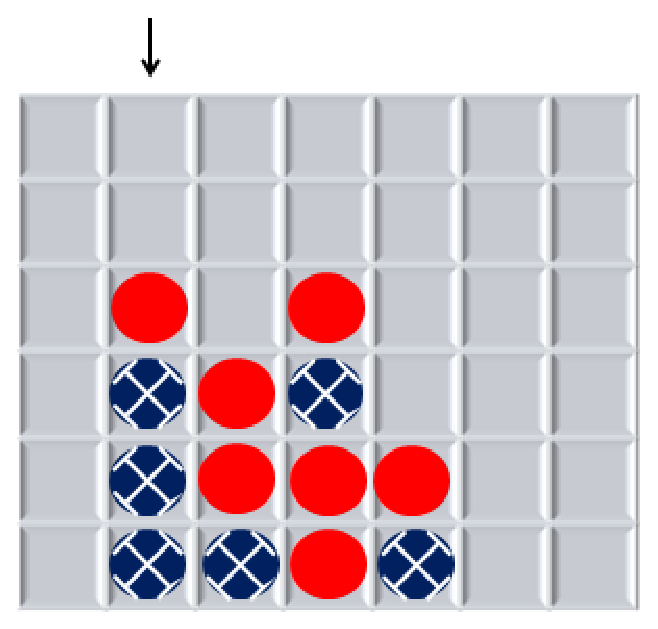
\includegraphics[scale=0.4]{contenido/cap7/imagenes/ckEstadoActualMovimiento.eps}
	\caption[Mejor movimiento de minimax y alfa-beta en el Conecta-4 (II)]{Mejor movimiento de minimax y alfa-beta para el estado de la figura~\ref{fig:comparativa_minimax_alfabeta2}.}
	\label{fig:comparativa_minimax_alfabeta2Movimiento}
\end{figure} 

\subsection{Monte-Carlo y Monte-Carlo Tree Search}
\label{ssec:comparativa_mcVSmctreesearch}
Este apartado compara las dos estrategias que usan el método de Monte-Carlo.
Para ello se estudian los resultados de enfrentar ambas estrategias en función del límite de tiempo disponible para decidir el mejor movimiento.

Se considera el juego del Conecta-4 en un tablero 6x7.
Cada prueba consiste en 100 partidas con un límite de tiempo para cada jugador a la hora de decidir los movimientos.
Para cada prueba se incrementa el límite de tiempo en un segundo, salvo para la última prueba que tiene un límite de 15 segundos.\footnote{Cada una de las pruebas puede durar varias horas, de ahí que se haya escogido el juego del Conecta-4 en lugar del juego del Go para realizar este experimento; incluso en el juego del Conecta-4 en un tablero 6x7 la duración media de cada prueba ha sido de 4 horas.}

En el primer caso, el jugador que mueve en primer lugar usa el método de Monte-Carlo básico y el segundo jugador el método Monte-Carlo Tree Search.
La tabla~\ref{tab:comparativa_montecarlo1} muestra los resultados de las pruebas realizadas.
La figura~\ref{fig:comparativa_montecarlo1} muestra estos datos de forma gráfica.

En el siguiente caso, el primer jugador usa el método Monte-Carlo Tree Search y el segundo jugador el método básico de Monte-Carlo.
Los resultados de esta pruebas se muestran en la tabla~\ref{tab:comparativa_montecarlo2} y en la figura~\ref{fig:comparativa_montecarlo2}.

En ambos casos, jugando como primer jugador o como segundo jugador, se observa claramente que el método Monte-Carlo Tree Search obtiene mejores resultados que el método Monte-Carlo basado simplemente en las simulaciones.

\begin{table}[!h]
\centering
\caption[Comparativa de los métodos de Monte-Carlo (I)]{Comparativa del método Monte-Carlo frente a Monte-Carlo Tree Search.}
\label{tab:comparativa_montecarlo1}
\begin{tabular}{cccc}
\hline
\textbf{Límite de tiempo (s)} & \textbf{Gana jug.1 (MC)} & \textbf{Empate} & \textbf{Gana jug.2 (MC Tree Search)}\\
%\hline
1 & 16\% &	5\% &	79\% \\
2 & 12\% &	1\% &	87\% \\
3 & 11\% &	1\% &	88\% \\
4 & 3\% &	0\% &	97\%  \\
5 & 3\% &	1\% &	96\%  \\
6 & 4\% &	2\% &	94\%  \\
7 & 4\% &	0\% &	96\%  \\
8 & 3\% &	1\% &	96\% \\
9 & 3\% &	1\% &	96\%  \\
10 & 3\% &	3\% &	94\% \\
15 & 1\% &	0\% &	99\% \\
\hline
\end{tabular}
\end{table} 

\begin{figure}[!h]
	\centering
	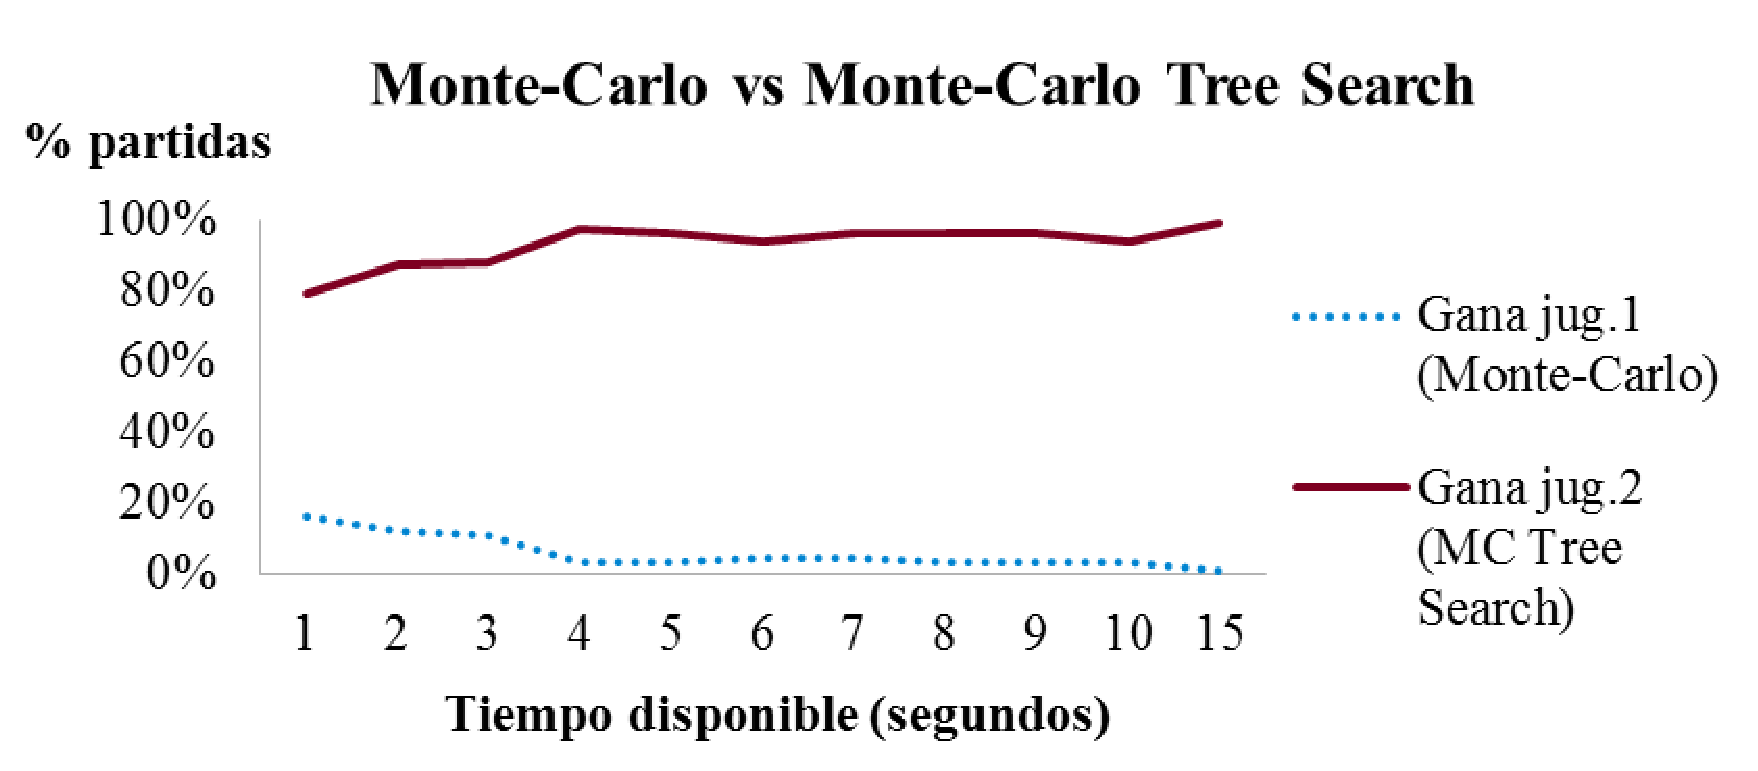
\includegraphics[scale=0.4]{contenido/cap7/imagenes/montecarlo1.eps}
	\caption[Comparativa de los métodos de Monte-Carlo (I)]{Gráfica comparativa de los métodos de Monte-Carlo (datos de la tabla~\ref{tab:comparativa_montecarlo1}).}
	\label{fig:comparativa_montecarlo1}
\end{figure} 

\begin{table}[!h]
\centering
\caption[Comparativa de los métodos de Monte-Carlo (II)]{Comparativa del método Monte-Carlo Tree Search frente a Monte-Carlo.}
\label{tab:comparativa_montecarlo2}
\begin{tabular}{cccc}
\hline
\textbf{Límite de tiempo (s)} & \textbf{Gana jug.1 (MC Tree Search)} & \textbf{Empate} & \textbf{Gana jug.2 (MC)}\\
%\hline
1 & 79\% &	3\% &	18\% \\
2 & 83\% &	6\% &	11\% \\
3 & 90\% &	7\% &	3\% \\
4 & 87\% &	6\% &	7\% \\
5 & 96\% &	4\% &	0\% \\
6 & 94\% &	4\% &	2\% \\
7 & 95\% &	2\% &	3\% \\
8 & 95\% &	3\% &	2\% \\
9 & 98\% &	2\% &	0\% \\
10 & 98\% &	1\% &	1\% \\
15 & 99\%	& 1\%	 & 0\% \\
\hline
\end{tabular}
\end{table} 

\begin{figure}[!h]
	\centering
	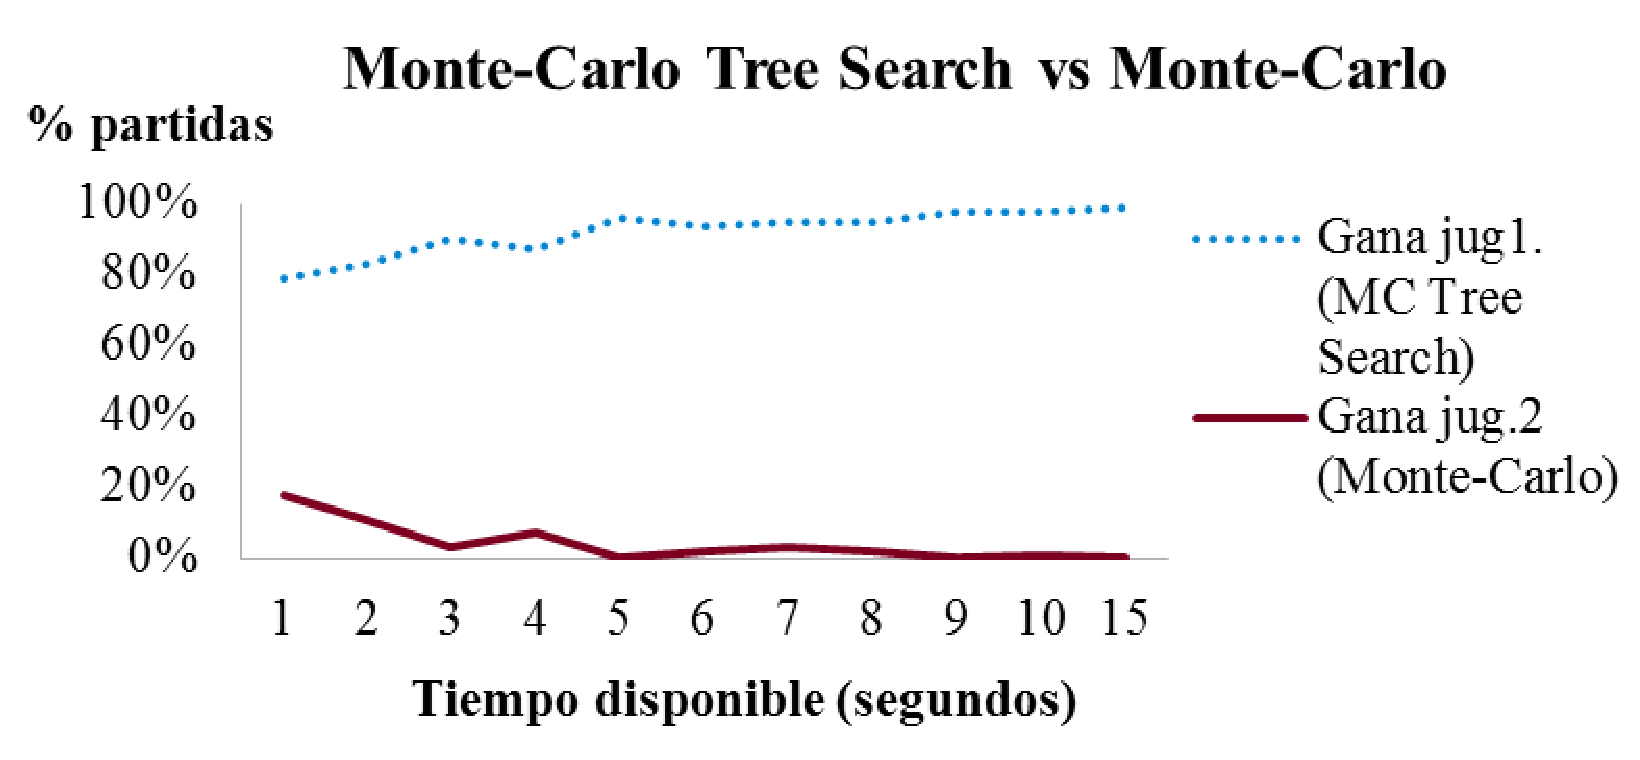
\includegraphics[scale=0.4]{contenido/cap7/imagenes/montecarlo2.eps}
	\caption[Comparativa de los métodos de Monte-Carlo (I)]{Gráfica comparativa de los métodos de Monte-Carlo (datos de la tabla~\ref{tab:comparativa_montecarlo2}).}
	\label{fig:comparativa_montecarlo2}
\end{figure} 


\subsection{Comparativa de estrategias en el Go}
\label{ssec:comparativa_estrategias_go}
A continuación se realiza una comparativa de varias estrategias en el juego del Go.

Se considera un tablero 9x9 inicialmente vacío, con las reglas de puntuación japonesas y sin puntos de ventaja para el segundo jugador.
Las estrategias a comparar son un jugador aleatorio, un jugador evaluador heurístico (\texttt{JugadorEvaluar}), un jugador minimax, un jugador con poda alfa-beta, un jugador Monte-Carlo y otro Monte-Carlo Tree Search.
El heurístico empleado tanto para el jugador evaluador heurístico como para minimax y alfa-beta ha sido el evaluador basado en la puntuación según las reglas japonesas.
Todas las estrategias (salvo el \texttt{JugadorEvaluar}) disponen de un segundo para encontrar el mejor movimiento.

La tabla~\ref{tab:comparativa_estrategias1} presenta los resultados de las pruebas para el caso en el que las estrategias juegan como primer jugador.
Cada estrategia ha jugado 100 partidas frente a un jugador aleatorio.
La figura~\ref{fig:comparativa_estrategias1} muestra de forma gráfica los resultados obtenidos.

Los resultados de las estrategias cuando son usadas por el segundo jugador se muestran en la tabla~\ref{tab:comparativa_estrategias2}.
La figura~\ref{fig:comparativa_estrategias2} muestra de forma gráfica estos resultados.
En este caso también se han jugado 100 partidas con cada estrategia frente a un jugador aleatorio.

\begin{table}[t]
\centering
\caption[Comparativa de estrategias en el Go (I)]{Comparativa de las estrategias usadas por el primer jugador en el Go.}
\label{tab:comparativa_estrategias1}
\begin{tabular}{lcccccc}
\hline
\textbf{Jugador 1:} & \textbf{Aleatorio} & \textbf{Ev. Heur.} & \textbf{Minimax} & \textbf{Alfa-Beta} & \textbf{MC} & \textbf{MC Tree Search} \\
%\hline
\textbf{Gana} & 47\% & 98\% & 89\% & 96\% & 83\% & 88\% \\
\textbf{Empata} & 4\% & 1\% & 0\% & 0\% & 1\% & 2\% \\
\textbf{Pierde} & 49\% & 1\% & 11\% & 4\% & 16\% & 10\% \\
\hline
\end{tabular}
\end{table} 

\begin{figure}[!h]
	\centering
	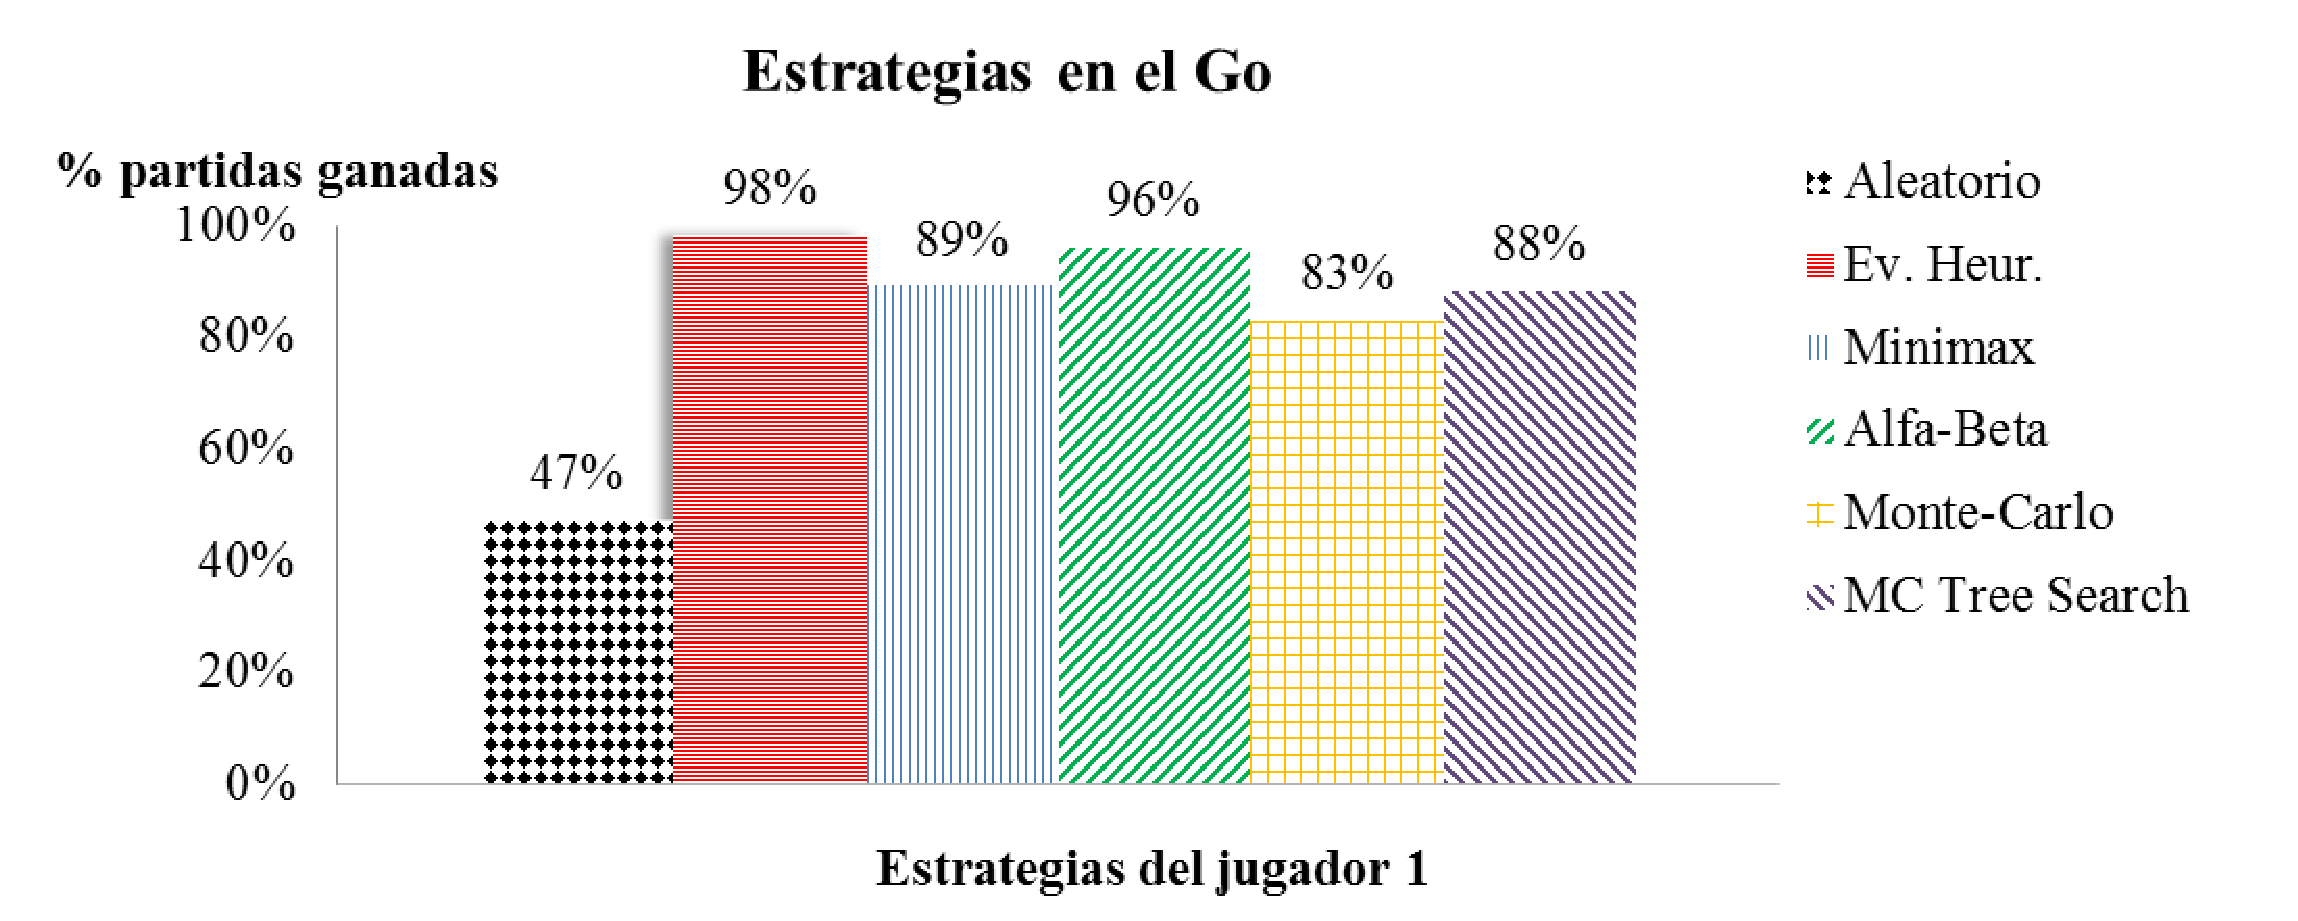
\includegraphics[scale=0.3]{contenido/cap7/imagenes/estrategiasGo1.eps}
	\caption[Comparativa de estrategias en el Go (I)]{Gráfica comparativa de las estrategias del primer jugador en el juego del Go.}
	\label{fig:comparativa_estrategias1}
\end{figure} 

\begin{table}[t]
\centering
\caption[Comparativa de estrategias en el Go (II)]{Comparativa de las estrategias usadas por el segundo jugador en el Go.}
\label{tab:comparativa_estrategias2}
\begin{tabular}{lcccccc}
\hline
\textbf{Jugador 2:} & \textbf{Aleatorio} & \textbf{Ev. Heur.} & \textbf{Minimax} & \textbf{Alfa-Beta} & \textbf{MC} & \textbf{MC Tree Search} \\
%\hline
\textbf{Gana} & 49\% & 94\% & 87\%  & 89\% & 80\% & 64\% \\
\textbf{Empata} & 4\% & 0\% & 1\% & 0\% & 0\% & 2\% \\
\textbf{Pierde} & 47\% & 6\%  & 12\% & 11\% & 20\% & 34\% \\
\hline
\end{tabular}
\end{table} 

\begin{figure}[!h]
	\centering
	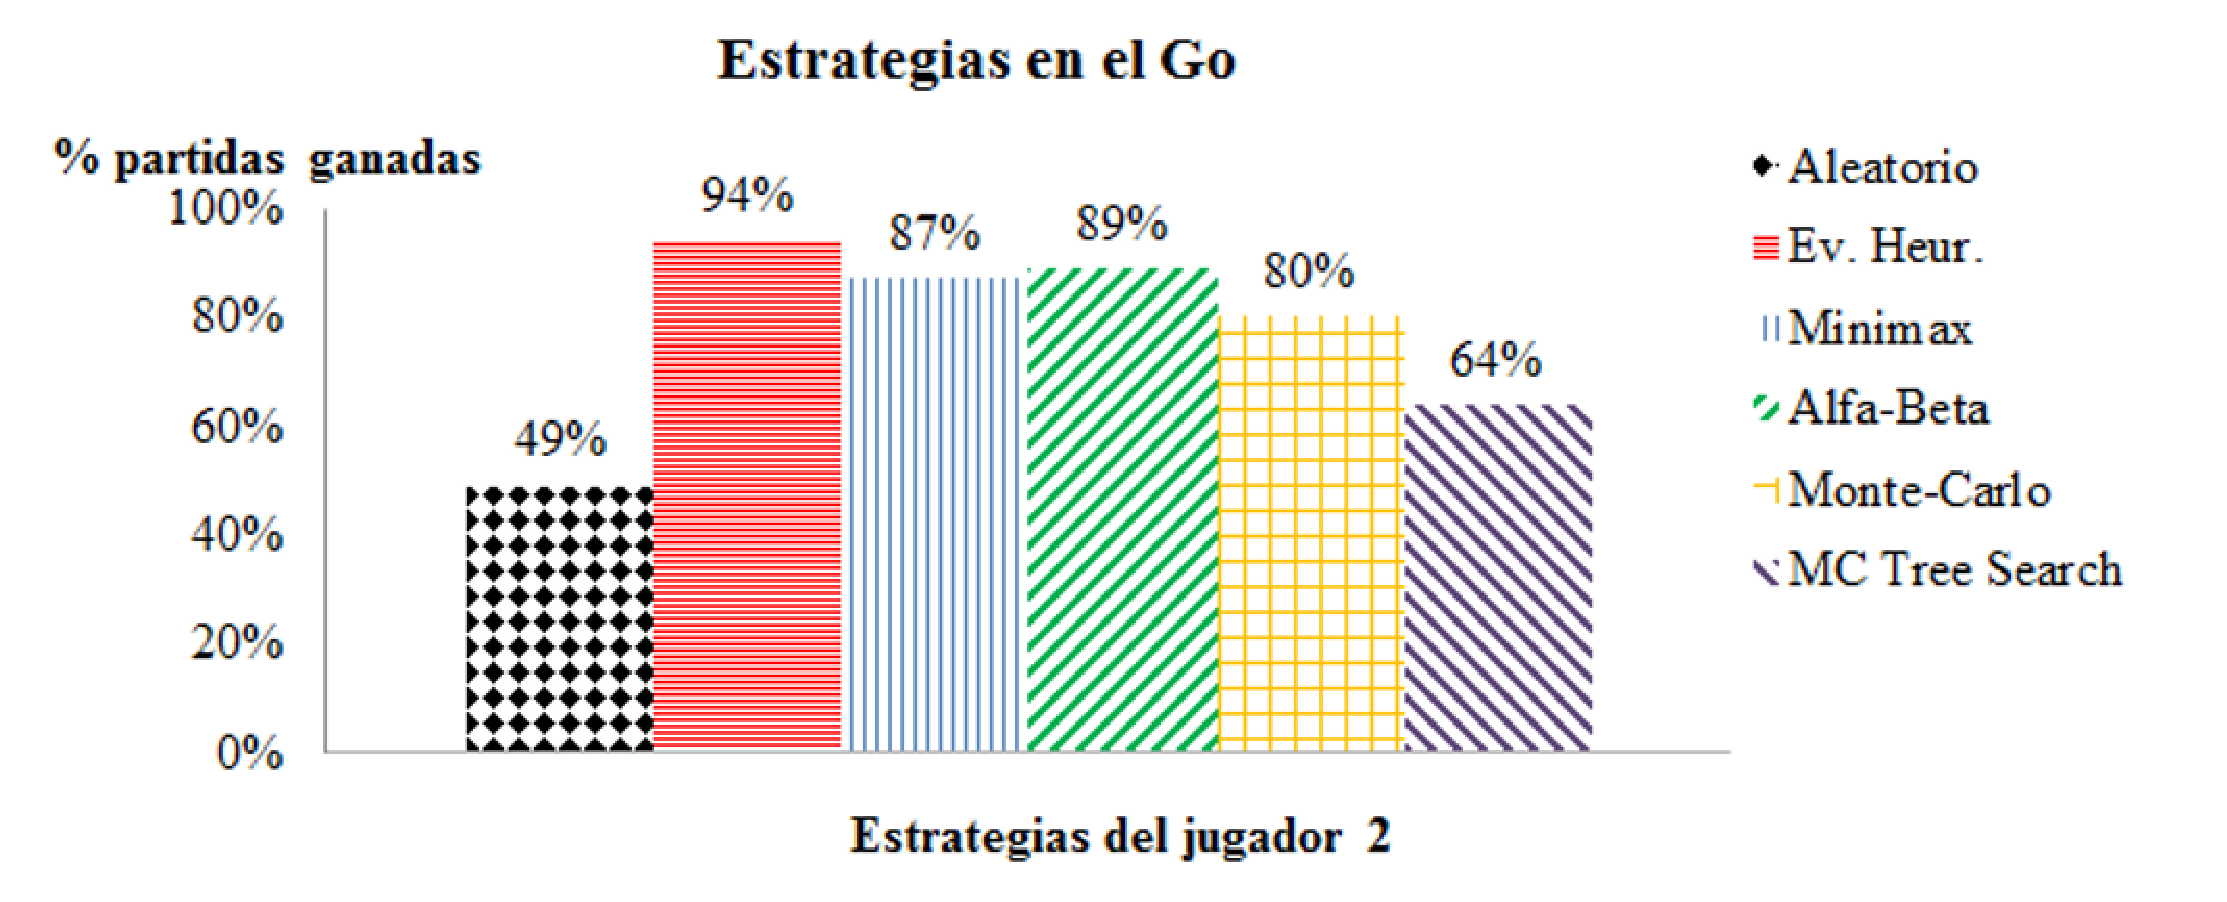
\includegraphics[scale=0.3]{contenido/cap7/imagenes/estrategiasGo2.eps}
	\caption[Comparativa de estrategias en el Go (II)]{Gráfica comparativa de las estrategias del segundo jugador en el juego del Go.}
	\label{fig:comparativa_estrategias2}
\end{figure} 

El evaluador heurístico (\texttt{JugadorEvaluar}) obtiene mejores resultados que minimax y alfa-beta porque examina completamente el primer nivel del árbol de estados.
Minimax y alfa-Beta realizan la búsqueda del mejor movimiento primero en profundidad y en un sólo segundo no les da tiempo a examinar el primer nivel completo.

El método de Monte-Carlo básico obtiene mejores resultados en este caso que Monte-Carlo Tree Search.
Esto se debe a que las simulaciones de Monte-Carlo Tree Search tardan más en ejecutarse que las simulaciones simples de Monte-Carlo.
Un único segundo es muy poco tiempo para realizar las simulaciones de Monte-Carlo Tree Search en un juego como el Go, ya que tanto el árbol de búsqueda como el árbol que se genera son enormes.
Aumentando el tiempo disponible se mejora esta estrategia igual que ocurría en el experimento de la sección~\ref{ssec:comparativa_mcVSmctreesearch}.


% 7. Conclusiones y trabajo futuro
\chapter{Conclusiones y trabajo futuro}
\label{cap:conclusiones}
Este capítulo presenta las conclusiones obtenidas tras el desarrollo del proyecto.
También describe el trabajo futuro relacionado con el proyecto como posibles extensiones o aplicaciones en otros campos de la IA.

\section{Conclusiones}
\label{sec:conclusiones}
Se han alcanzado plenamente los objetivos del proyecto: desarrollar un entorno interactivo para estudiar las estrategias de IA en los juegos.
La aplicación desarrollada permite ver en funcionamiento las estrategias de juegos, pudiendo jugar contra ellas y simplificando la tarea de analizarlas y compararlas.
Se trata, por lo tanto, de una herramienta didáctica que puede resultar muy útil de cara a la docencia, tanto para los alumnos como para los profesores.

La búsqueda de una estrategia óptima en juegos es un problema intratable en la mayoría de los casos, todos los algoritmos deben hacer algunas suposiciones y aproximaciones.
Los algoritmos vistos son solamente algunas formas de aproximarse a la estrategia óptima.
Cada estrategia tiene sus ventajas e inconvenientes, por ejemplo minimax garantiza una estrategia ganadora si pudiera aplicarse al árbol de juegos completo, pero como esto no es posible en la práctica, da lugar a varios inconvenientes como el \textit{efecto horizonte}\footnote{Efecto que ocurre cuando se evalúa como buena o mala una posición sin saber que en la siguiente jugada la situación se revierte.} cuando la condición de corte del algoritmo está basada sólo en una profundidad fija.

Se han desarrollado y estudiado en detalle los algoritmos clásicos en sus versiones más básicas (minimax, alfa-beta y tablas de transposición), dejando de lado posibles mejoras más sofisticadas de estos como la búsqueda de la quietud (\textit{quiescence search}), los números de conspiración (\textit{conspiracy numbers}), la búsqueda con ventana cero (\textit{zero window search}) o las bases de datos de aperturas y de finales,\footnote{Puede obtenerse más información sobre estos conceptos en~\citeref{IAICJMHA}.} aunque el proyecto permite agregar estas estrategias de forma sencilla.

También se han estudiado otros métodos más recientes como Monte-Carlo Tree Search, basado en el clásico método de Monte-Carlo.
A su vez, se han visto una rama de la IA como es el aprendizaje en máquinas, aplicado a los agentes de juegos; permitiendo entrenar redes neuronales capaces de aprender a jugar al Conecta-4 y al Go.

Como curiosidad mencionar una pequeña experiencia que tuve durante el proyecto en mi búsqueda de empleo: una empresa británica relacionada con las apuestas deportivas por Internet me propuso como ejercicio de evaluación el desarrollo del juego del 3 en raya junto con un jugador inteligente, usando el lenguaje Java.
No había ninguna restricción en cuanto a la estrategia del jugador, pero la única condición que debía cumplir es que nunca perdiera frente a la estrategia propuesta por ellos.
La estrategia Monte-Carlo en su versión básica con 1.000 simulaciones por movimiento fue suficiente para cumplir el objetivo.

\section{Trabajo futuro}
\label{sec:trabajo_futuro}
Como trabajo futuro se presentan algunas extensiones y mejoras del proyecto realizado que pueden dar lugar a otros proyectos de investigación en el ámbito de la IA y la ingeniería del software.

\subsection{Extensiones del proyecto}
\label{ssec:extensiones_proyecto}
A parte de la extensión natural del proyecto incorporando nuevos juegos, estrategias y heurísticos como se muestra en el apéndice~\ref{cap:desarrollo_juegos_estrategias_heuristicos}, el proyecto queda abierto a otro tipo de extensiones y mejoras de mayor envergadura.
A continuación se exponen algunas de ellas ordenadas de mayor a menor relevancia:

\begin{itemize}
	\item Adaptación del módulo de razonamiento a otras clases de juegos: multijugador, de suma no cero, de información imperfecta e indeterministas.

	Aunque el proyecto esta enfocado a los juegos clásicos de tablero, la extensión más natural del mismo es extender su aplicación a otros tipos de juegos con diferentes características.
	
	Esta extensión requiere rediseñar el módulo de razonamiento además de adaptar todas las estrategias a las nuevas características de los juegos; teniendo en cuenta que no todos los algoritmos vistos son generalizables para las nuevas características. 
	Esta extensión puede considerarse un proyecto aparte debido a su alcance y complejidad.		
	
	\item Mejoras de los algoritmos con versiones concurrentes de los mismos.

	Con la consolidación de la tecnología Grid y los procesadores paralelos se dispone de mayores recursos (cómputo y almacenamiento) para mejorar las decisiones de los algoritmos clásicos; además de desarrollar nuevos algoritmos basados en la programación distribuida.
	
	\item Modificación de la aplicación interactiva para incorporar nuevos juegos, estrategias y heurísticos en tiempo de ejecución.
	
	Esta modificación, aunque pueda parecer una mejora obvia y deseada en la aplicación, supone una tarea compleja de llevar a cabo, debido a que se debe dividir las diferentes partes del módulo de razonamiento de forma que puedan compilarse por separado y después conectarse a la aplicación.
	Se trata de un desarrollo basado en componentes.	

	Dentro de esta extensión también puede considerarse la posibilidad de que los nuevos componentes sean desarrollados con diferente tecnología o que sean independientes del lenguaje de programación.
	% Esto supone cambiar el diseño arquitectónico del proyecto por un desarrollo basado en componentes.
		
\end{itemize}

Personalmente la primera extensión es la más atractiva, pues expande el ámbito de los juegos con las nuevas características de los mismos, sobre todo con el auge actual de los juegos modernos de tablero (\textit{modern board-games} o \textit{Eurogames}); esto obliga a estudiar e investigar nuevas estrategias o modificar las existentes para ajustarse a dichas características.

\subsection{Aplicación a otras áreas}
\label{ssec:aplicacion_areas}
Los juegos se han representado como problemas de búsqueda con adversarios y los algoritmos estudiados están enfocados a ese tipo de problemas.
Sin embargo, estos algoritmos se pueden extender a otras áreas de la Inteligencia Artificial o de la Investigación Operativa como por ejemplo la generación de planes o los problemas de decisión.

También ocurre el proceso inverso, es decir, que se adapten algoritmos de otras áreas al ámbito de los juegos, como es el caso del método de Monte-Carlo, usado en infinidad de campos (economía, finanzas \citeref{glasserman2004monte}, física médica, procesamiento de gráficos \citeref{GPUMonteCarlo} o incluso para calcular el número \textit{pi}). 
En \citeref{george1996monte} puede encontrarse más aplicaciones del método de Monte-Carlo.

En ambos casos, las continuas innovaciones en el ámbito de los juegos generan entusiasmo y resultan relevantes para las investigaciones en IA.

% Apéndices
% A. Manual de usuario
\appendix
\clearpage % o \cleardoublepage
\addappheadtotoc
\appendixpage

\chapter{Manual de usuario}
\label{cap:manualUsuario}
Este apéndice es el manual de usuario del entorno interactivo.
Muestra la instalación de la aplicación y explica el funcionamiento de la misma.

\section{Instalación}
\label{sec:instalacion}
\par
El entorno interactivo no necesita de un proceso de instalación.
Se trata de un archivo \textit{JAR} (\textit{Java Archive}), lo que facilita la distribución de la aplicación.

\subsection{Requisitos mínimos}
\label{ssec:requisitos_minimos}
El requisito mínimo para la ejecución de la aplicación es:
\begin{itemize}
  \item Tener instalada la Máquina Virtual de Java (JVM) en su versión 1.6 o superior.\\
	Se puede obtener gratuitamente en: \texttt{http://www.java.com/es/download/index.jsp}
\end{itemize}

\section{Ejecución}
La aplicación se puede ejecutar simplemente haciendo doble clic sobre el fichero \textit{JAR}.
También es posible ejecutarlo desde un terminal de línea de comandos con la siguiente instrucción:
\texttt{java -jar <<aplicación.jar>>}

\section{Funcionamiento}
\label{sec:funcionamiento}
Tanto el aspecto de la aplicación como su funcionamiento son fáciles de entender. 
Todas la ventanas de la aplicación contienen en su parte inferior una zona dedicada a mostrar información de ayuda sobre el componente de la ventana en el que se sitúa el usuario con el puntero del ratón.

El programa dispone de una pantalla principal dividida en tres partes: los juegos, las estrategias y las funciones principales.
La figura~\ref{fig:ventana_principal} muestra la ventana principal.

\begin{figure}[!h]
	\centering
	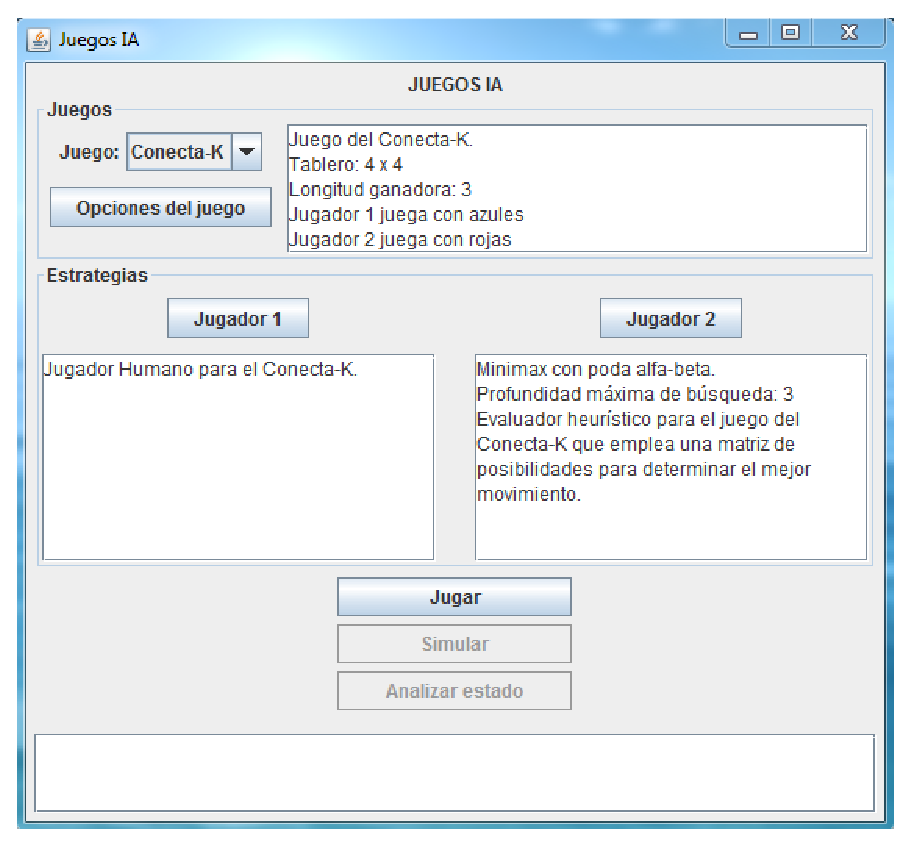
\includegraphics[scale=0.4]{contenido/apendiceA/imagenes/ventanaPrincipal.eps}
	\caption{Pantalla principal de la aplicación.}
	\label{fig:ventana_principal}
\end{figure}

La parte de los juegos nos permite seleccionar y configurar un juego; la parte de estrategias se encarga de seleccionar, configurar y entrenar si es necesario las estrategias de los dos jugadores y por último tenemos los tres modos de uso de la aplicación: jugar, simular y analizar estado.

Estas partes están organizadas de arriba a abajo, pues el orden de uso es importante: primero se debe elegir y configurar el juego, a continuación las estrategias de los dos jugadores y por último elegir la acción deseada.
Esto es así porque las estrategias pueden necesitar información del juego y este último debe estar configurado previamente.
Si seleccionamos un juego después de configurar las estrategias, las estrategias se restablecerán a sus valores por defecto.

\subsection{Selección y configuración del juego}
\label{ssec:funcionamiento_juegos}
Se puede seleccionar un juego directamente desde la pantalla principal de la aplicación; junto a él se muestra información del juego y su configuración por defecto.

Si se desea cambiar la configuración del juego debemos seleccionar la opción \texttt{``Opciones del juego''}.
Se accede a una nueva ventana con diferentes opciones de configuración que dependen del juego seleccionado.
Para obtener ayuda sobre estas opciones hay que situar el puntero del ratón sobre las mismas y se obtendrá información sobre ella en la parte inferior de la ventana.

\subsection{Selección y configuración de los jugadores}
\label{ssec:funcionamiento_jugadores}
La parte central de la ventana principal esta dividida a su vez en dos partes: una dedicada al primer jugador y otra al segundo jugador.
Cada una de ellas muestra información sobre la estrategia actual seleccionada para el jugador.
La estrategia por defecto es un jugador humano.
Pulsando los botones \texttt{``Jugador 1''} y \texttt{``Jugador 2''} podemos cambiar y configurar las estrategias para cada jugador.

La figura~\ref{fig:ventana_estrategia} muestra la ventana de configuración de las estrategias; esta ventana es idéntica para ambos jugadores.
Contiene una lista con las estrategias disponibles; al seleccionar una estrategia se muestra al lado información sobre la misma y la parte inferior de la ventana cambia para mostrar las opciones de configuración de esa estrategia.\footnote{No todas las estrategias son configurables.}

\begin{figure}[!h]
	\centering
	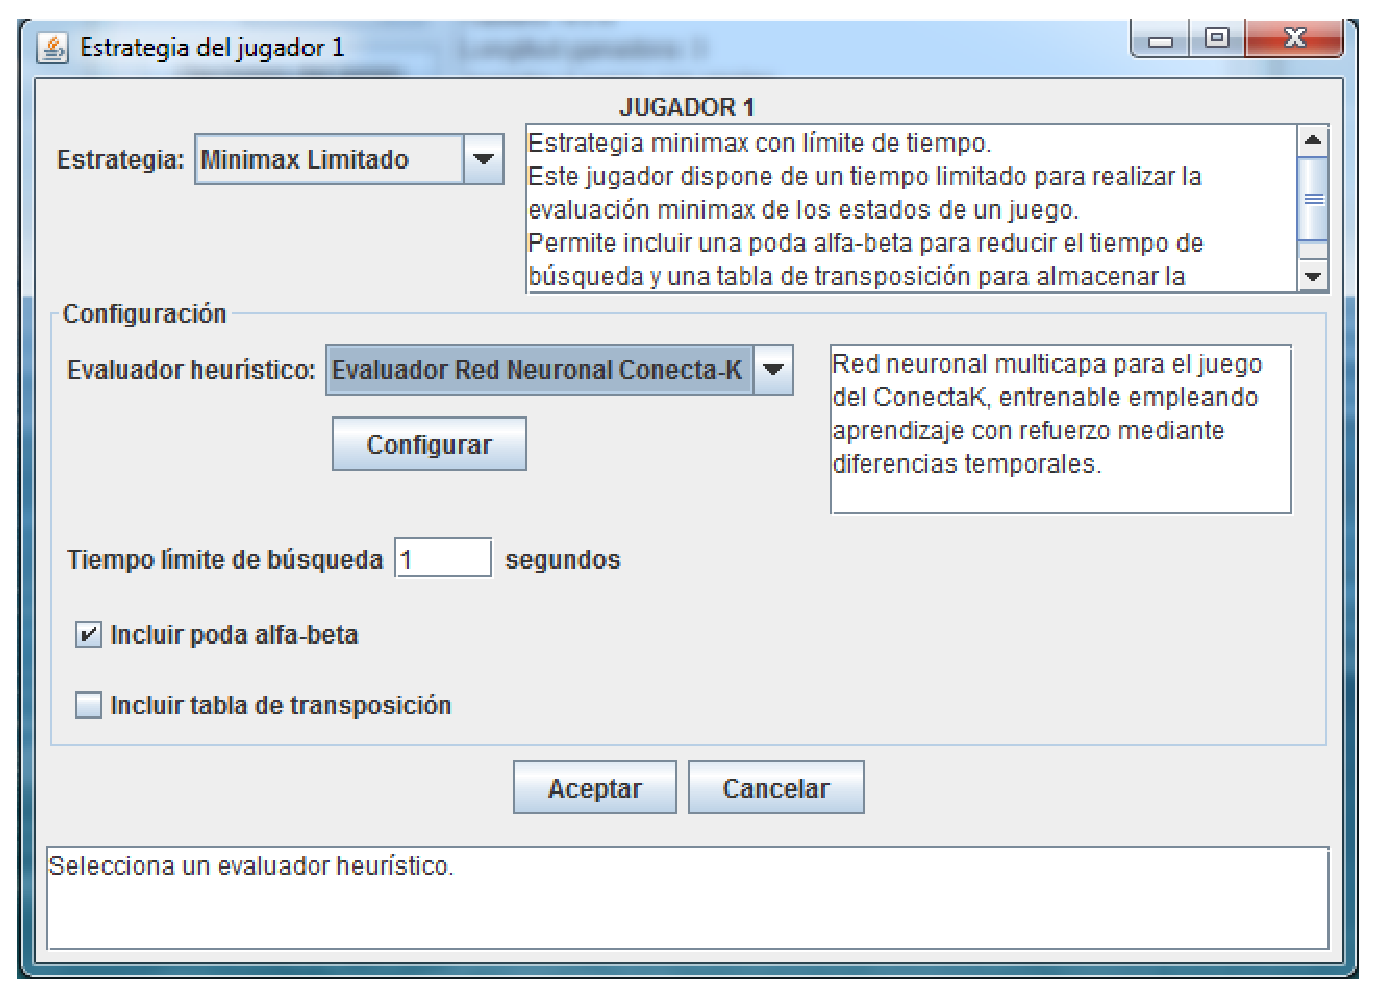
\includegraphics[scale=0.4]{contenido/apendiceA/imagenes/ventanaEstrategias.eps}
	\caption{Pantalla de selección y configuración de la estrategia.}
	\label{fig:ventana_estrategia}
\end{figure}

La opción más interesante es la selección y configuración de un evaluador heurístico para las estrategias.
Esta opción sólo estará disponible en las estrategias que necesiten de un heurístico para evaluar las posiciones de los juegos.
Por otro lado también hay heurísticos que no necesitan configurar sus parámetros.

En el caso de que el heurístico permita configurar sus parámetros se activa la opción \texttt{``Configurar''} debajo del heurístico seleccionado.
Esta opción da acceso a una nueva ventana como la que se muestra en la figura~\ref{fig:ventana_evaluador}.

\begin{figure}[!h]
	\centering
	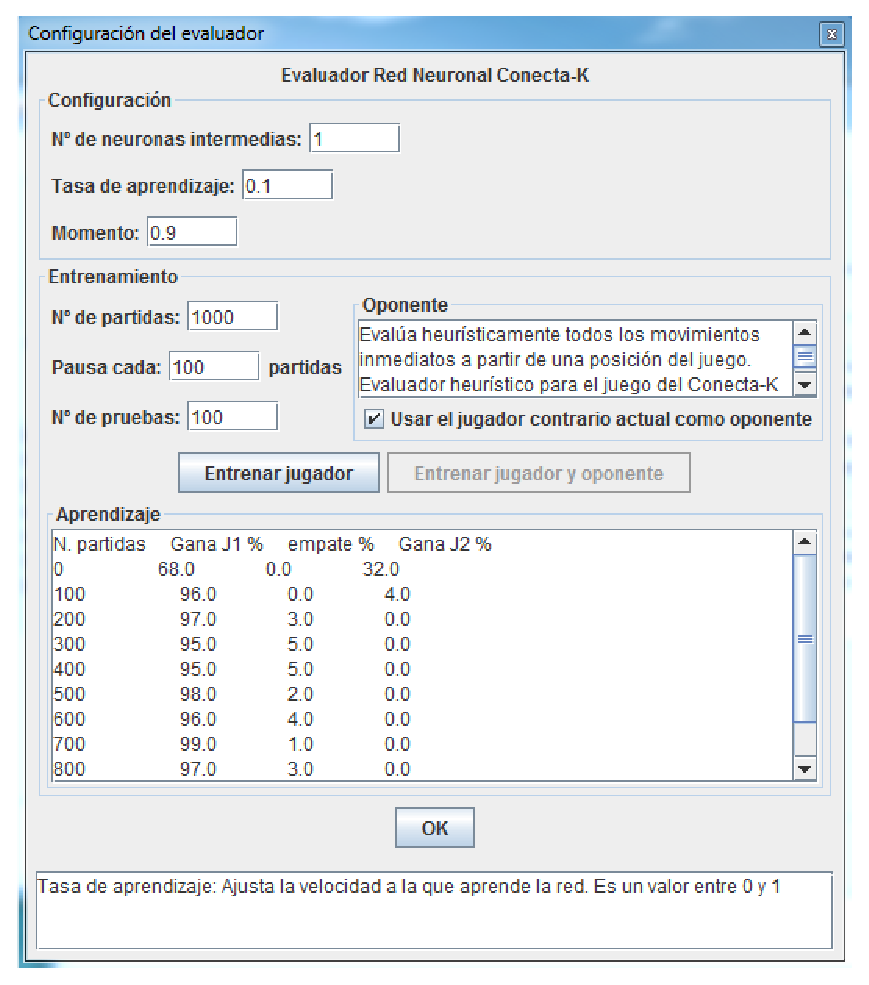
\includegraphics[scale=0.5]{contenido/apendiceA/imagenes/ventanaEvaluador.eps}
	\caption{Pantalla de configuración y entrenamiento de un evaluador heurístico.}
	\label{fig:ventana_evaluador}
\end{figure}

La parte superior muestra los parámetros de configuración del evaluador heurístico, mientras que la parte inferior permite entrenar el evaluador.
La parte de entrenamiento sólo se mostrará si el evaluador es entrenable; en caso contrario la ventana sólo mostrará los parámetros de configuración del evaluador.

\subsubsection{Entrenamiento del jugador}
\label{sssec:entrenamiento_jugador}
La ventana de configuración del evaluador permite entrenar al evaluador heurístico y por tanto al jugador usando aprendizaje por refuerzo.

La parte inferior de la ventana (figura~\ref{fig:ventana_evaluador}) muestra las opciones de entrenamiento.
Para entrenar al jugador se debe indicar el número de partidas de entrenamiento.
Los campos \texttt{``pausa cada \textit{n} partidas''} y \texttt{``número de pruebas''} permiten ver el desarrollo del aprendizaje.
Cada \textit{n} partidas de entrenamiento se realizará una pausa y se jugará el número de partidas de prueba indicado; el resultado de estas pruebas se irá mostrando en la parte inferior.

El entrenamiento se realiza por defecto frente a un oponente con estrategia aleatoria; pero también se puede entrenar frente al jugador contrario activando la opción \texttt{``Usar el jugador contrario actual como oponente''}.
Esta opción sólo se podrá activar si el jugador contrario es controlador por el ordenador, es decir, no es un jugador humano.

La misma ventana de entrenamiento también permite entrenar simultáneamente a los dos jugadores seleccionados.
Para ello el jugador contrario debe ser entrenable y debe activarse la opción \texttt{``Usar el jugador contrario actual como oponente''} comentada anteriormente.
Al activar esta opción aparece un nuevo botón \texttt{``Entrenar jugador y oponente''} que sólo estará activo si el jugador oponente también es entrenable.
Se entrenará simultáneamente a los dos jugadores, uno frente al otro, cada uno con su propia estrategia.

\subsection{Modos de uso de la aplicación}
\label{ssec:funcionalidad}
La aplicación tiene tres modos de uso básicos: jugar, simular y analizar estado.
A continuación se explica el funcionamiento de cada uno de estos modos.

\subsubsection{Jugar}
\label{sssec:jugar}
Esta opción nos permite jugar una partida al juego seleccionado.
Se puede jugar contra cualquier estrategia disponible o contra otro jugador humano.
En el caso de que ninguna de las estrategias sea un jugador humano, se mostrará el desarrollo de una partida entre los dos jugadores controlados por el ordenador.

La figura~\ref{fig:ventana_jugar} muestra el desarrollo de una partida de Go entre dos jugadores controlados por el ordenador.
La parte derecha muestra información sobre las estrategias y sobre el desarrollo de la partida (último movimiento, turno del jugador, puntuación,\ldots). La parte inferior muestra información sobre el movimiento actual, por ejemplo indicando si estamos sobre una posición sobre la que está prohibido mover.

\begin{figure}[!h]
	\centering
	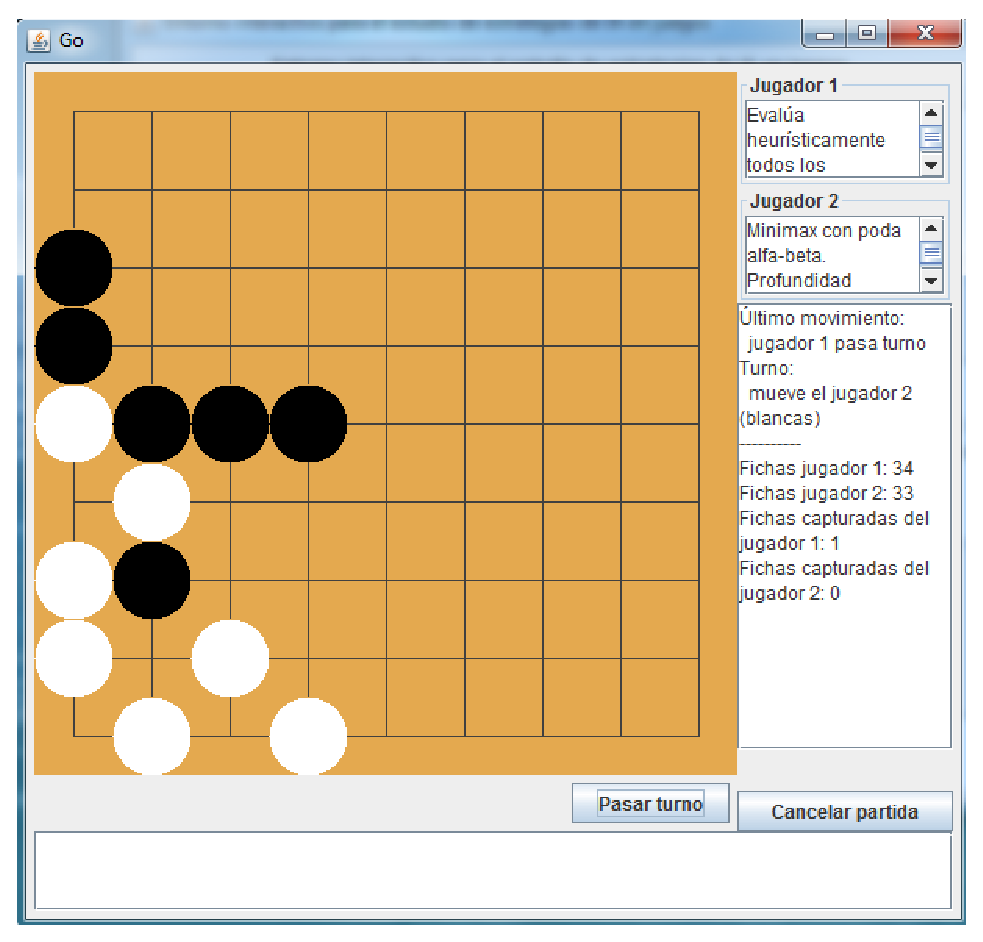
\includegraphics[scale=0.5]{contenido/apendiceA/imagenes/ventanaJuego.eps}
	\caption{Pantalla de juego.}
	\label{fig:ventana_jugar}
\end{figure}

Dependiendo de la estrategia usada, los movimientos de los jugadores pueden ser muy rápidos y el ojo humano no es capaz de seguir el desarrollo de la partida; para evitar esto se realiza una pequeña pausa de un segundo entre cada movimiento.
La partida puede cancelarse en cualquier momento, volviendo a la pantalla principal.

Cuando termina la partida se muestra la ventana de estadísticas con información acerca de la partida.

\subsubsection{Simular}
\label{sssec:simular}
La opción ``Simular'' consiste en realizar un número determinado de partidas entre dos jugadores controlados por el ordenador.
El desarrollo de estas partidas no es visible, pues el propósito de la simulación es comparar las estrategias con los resultados obtenidos a partir de todas las partidas jugadas.
La figura~\ref{fig:ventana_simulacion} muestra la ventana de simulación.

\begin{figure}[!h]
	\centering
	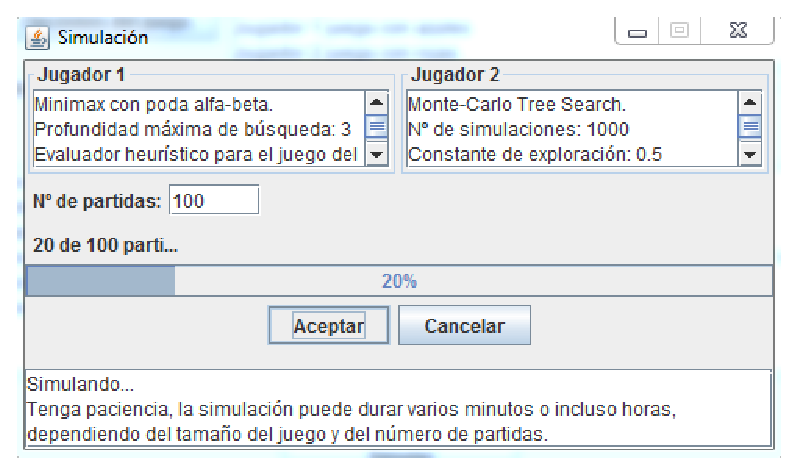
\includegraphics[scale=0.5]{contenido/apendiceA/imagenes/ventanaSimulacion.eps}
	\caption{Pantalla de simulación.}
	\label{fig:ventana_simulacion}
\end{figure}

Para realizar una simulación con éxito hay que tener en cuenta el tamaño del árbol de búsqueda del juego seleccionado y las estrategias elegidas porque una simulación puede durar desde segundos hasta horas, en función de estos factores y el número de partidas que se jueguen.
La simulación puede cancelarse en cualquier momento.
%En este caso no es posible detener la simulación una vez comenzada, pues se trata de un proceso intensivo en CPU y la interfaz queda deshabilitada.\footnote{Para cancelar una simulación se debe cerrar la aplicación desde un terminal de línea de comandos o mediante el administrador de tareas del sistema.}

Al finalizar la simulación se muestran las estadísticas de las partidas en una nueva ventana.

\subsubsection{Analizar estado}
\label{sssec:analizar_estado}
Esta opción permite al usuario construir un estado del juego seleccionado y a continuación estudiar el movimiento que realizaría cada uno de los jugadores en esa posición.

Para construir el estado el usuario debe realizar los movimientos oportunos de los dos jugadores, situando fichas en las posiciones deseadas pero siempre siguiendo las reglas del juego.
El usuario alternará los movimientos de ambos jugadores hasta conseguir el estado deseado.

La figura~\ref{fig:ventana_analisis} muestra la construcción de un estado para el juego del Conecta-4.
Una vez construido el estado deseado se debe pulsar la opción \texttt{``Analizar estado''} y los dos jugadores elegidos realizarán un movimiento; independientemente del turno del jugador, ambos jugadores realizan el mismo movimiento para comparar la decisión que toman las estrategias usadas por los jugadores.

\begin{figure}[!h]
	\centering
	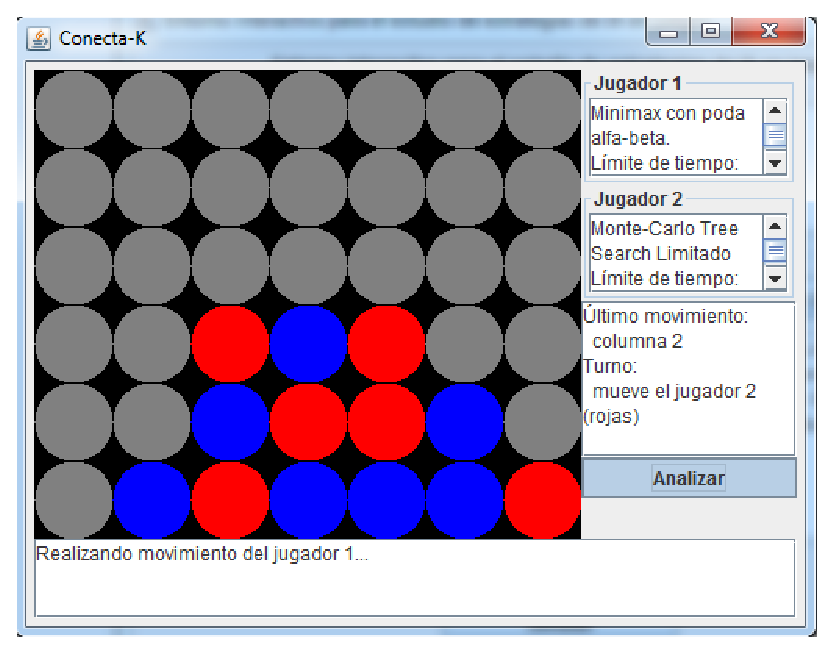
\includegraphics[scale=0.5]{contenido/apendiceA/imagenes/ventanaAnalisis.eps}
	\caption{Pantalla de análisis de estados.}
	\label{fig:ventana_analisis}
\end{figure}

Una vez finalizado el movimiento de los dos jugadores, se mostrará una nueva ventana con información de los movimientos realizados y estadísticas de las estrategias.

\subsection{Estadísticas}
\label{ssec:ventana_estadisticas}
Al finalizar cada uno de los modos de uso de la aplicación se mostrará una ventana con estadísticas.
La información mostrada en esta ventana depende del modo de uso elegido, aunque hay información común que es independiente del modo de uso y del jugador como el número de movimientos realizados o el tiempo medio de cada uno de los movimientos.

A continuación se describe brevemente la información mostrada para cada modo de uso de la aplicación:

\begin{description}
	\item[Jugar] (Figura~\ref{fig:subfig:ventana_estadisticas_jugar}) Al terminar de jugar una partida se muestra la situación del estado final, el último movimiento realizado, el resultado (el ganador), el tiempo de juego\footnote{El tiempo de juego incluye un segundo adicional por cada movimiento como se comentó en el apartado~\ref{sssec:jugar}.},\ldots
Los jugadores muestran estadísticas de sus estrategias para la partida completa.

	\item[Simular] (Figura~\ref{fig:subfig:ventana_estadisticas_simular}) En el caso de una simulación se muestra el porcentaje de partidas ganadas por cada jugador, el tiempo total de la simulación y el tiempo medio de cada partida.
Hay que prestar atención a la información mostrada por cada uno de los jugadores pues se trata de estadísticas acumuladas de todas las partidas.

	\item[Analizar estado] (Figura~\ref{fig:subfig:ventana_estadisticas_analizar}) Cuando termina el análisis se muestra el estado que ha sido analizado y los estados resultantes después de que los jugadores hayan movido.
	Cada estado puede mostrar información propia del mismo, aunque esta información depende del juego (último movimiento, puntuación actual de cada jugador,\ldots).
	Las estadísticas proporcionadas por los jugadores corresponden esta vez a un único movimiento.
	
\end{description}

\begin{figure}[h]
	\centering
	% Primera imagen
	\subfloat[]{
		\label{fig:subfig:ventana_estadisticas_jugar}
		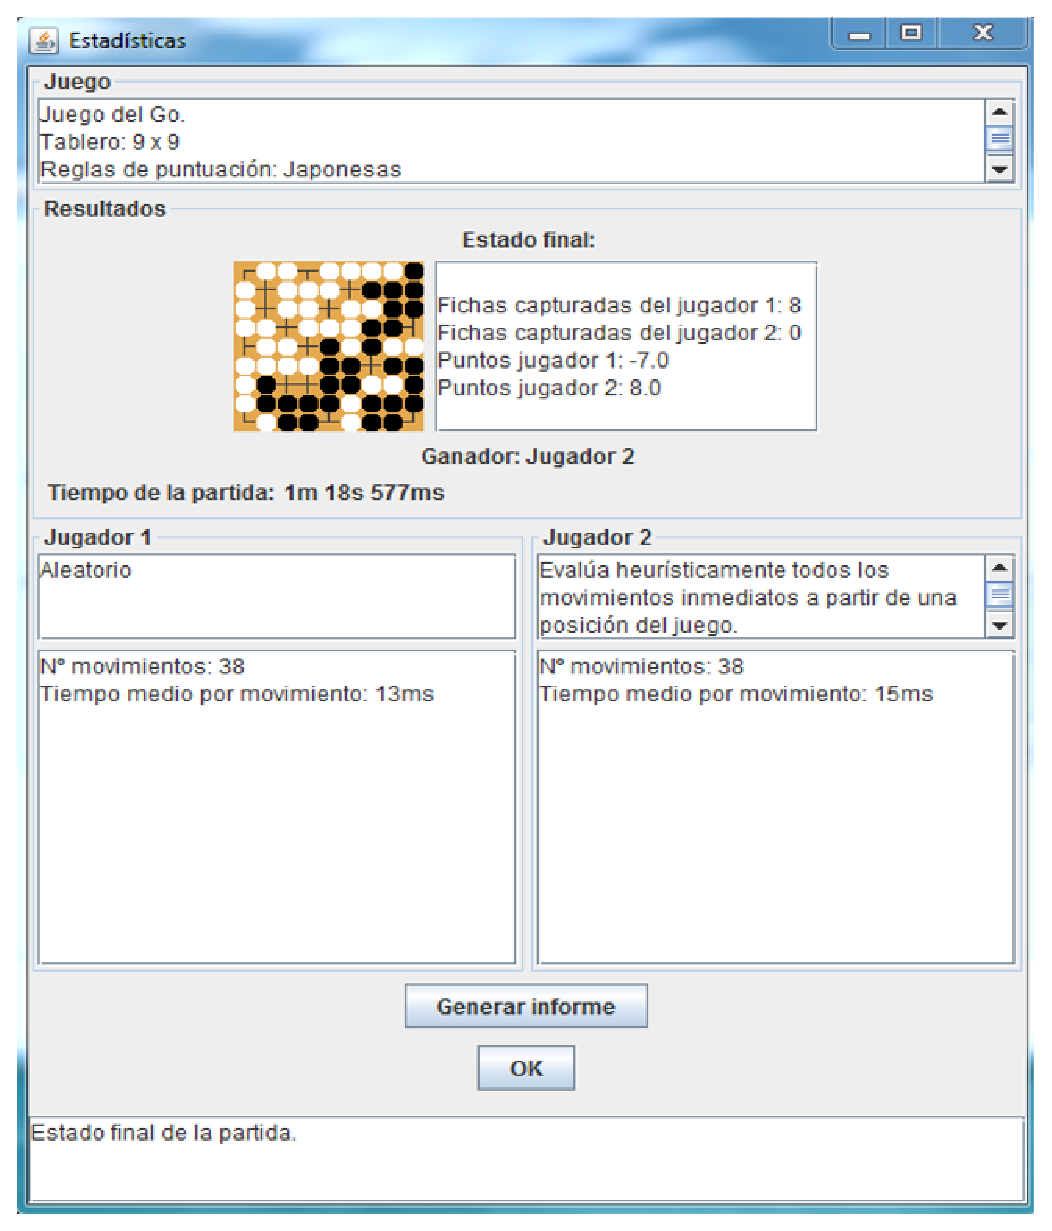
\includegraphics[scale=0.3]{contenido/apendiceA/imagenes/estadisticasJugar.eps}
	}
	\hspace{1cm}
	% Segunda imagen
	\subfloat[]{
		\label{fig:subfig:ventana_estadisticas_simular}
		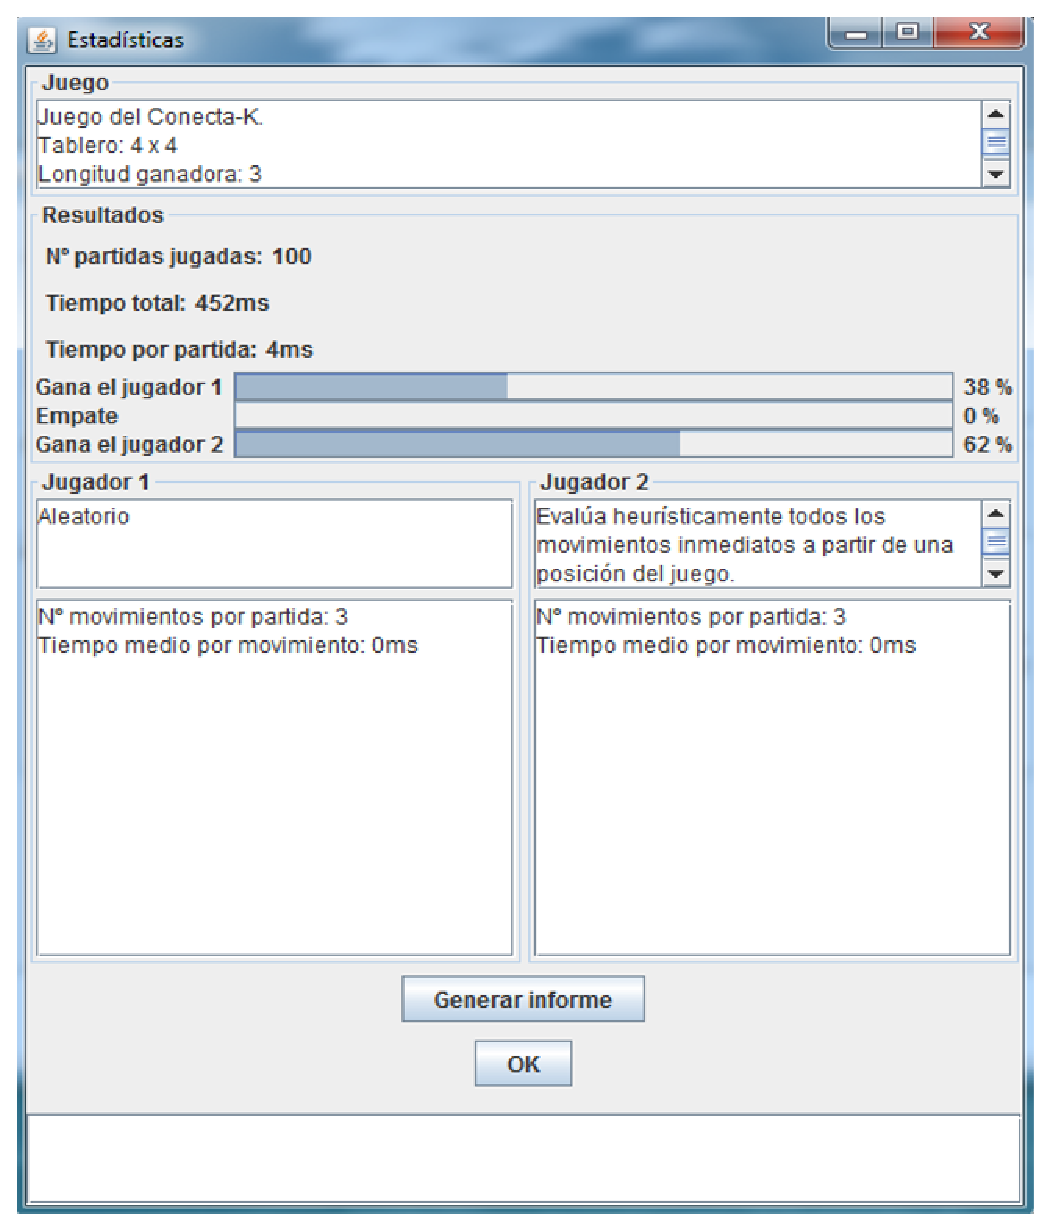
\includegraphics[scale=0.3]{contenido/apendiceA/imagenes/estadisticasSimulacion.eps}
	}
	\hspace{1cm}
	% Tercera imagen
	\subfloat[]{
		\label{fig:subfig:ventana_estadisticas_analizar}
		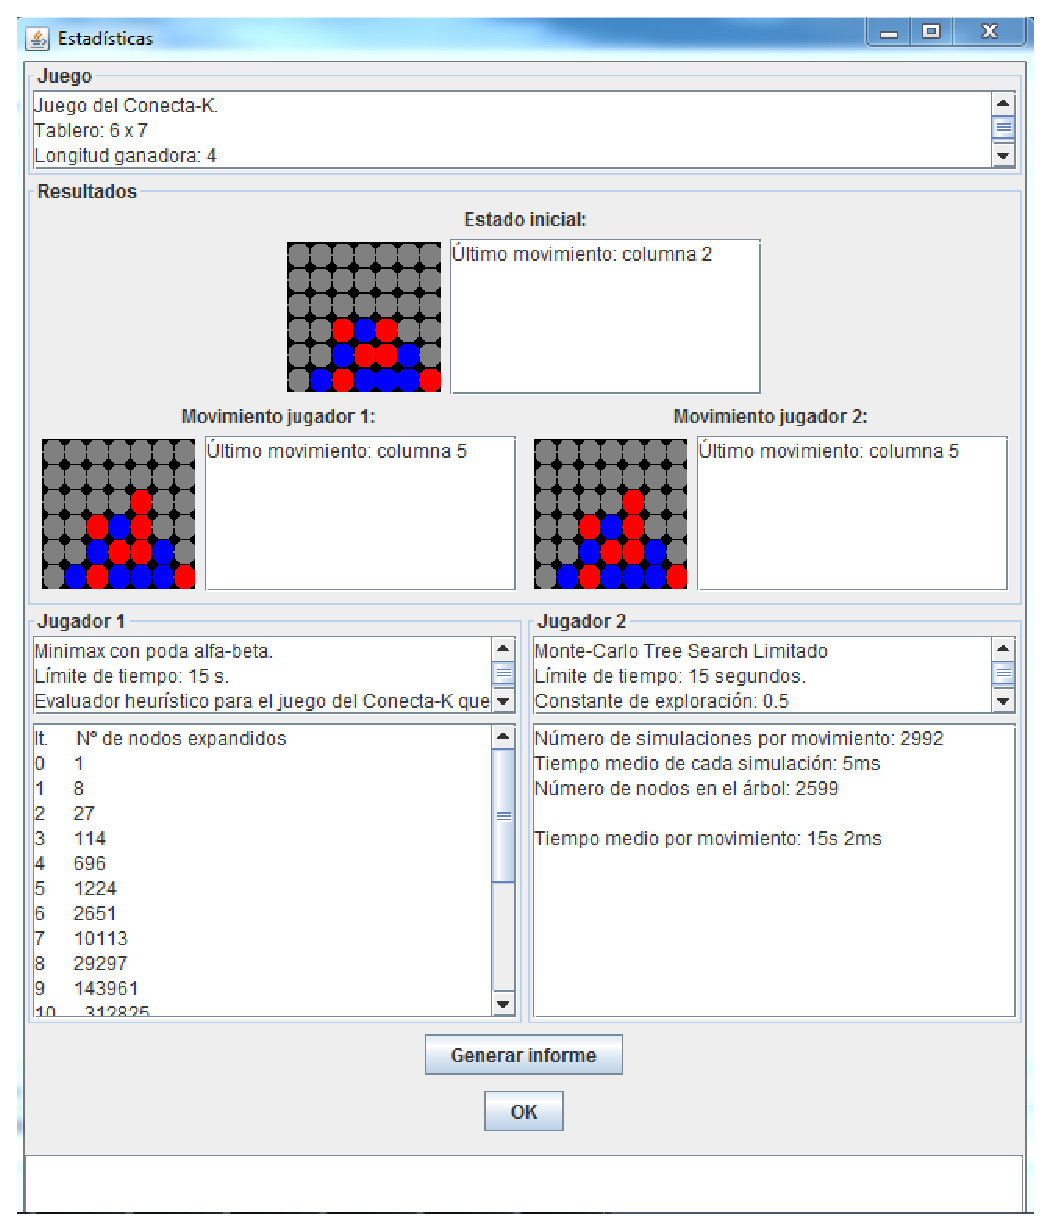
\includegraphics[scale=0.3]{contenido/apendiceA/imagenes/estadisticasAnalisis.eps}
	}
	\caption{Pantallas de resultados y estadísticas.}
	\label{fig:ventana_estadisticas}
\end{figure}

En todos los casos se puede generar un informe en formato texto plano con toda la información obtenida.
Para ello se debe seleccionar la opción \texttt{``Generar informe''}.











% B. Desarrollo de nuevos juegos, estrategias y heurísticos.
%\appendix
%\clearpage % o \cleardoublepage
%\addappheadtotoc
%\appendixpage

\chapter{Desarrollo de nuevos juegos, estrategias y heurísticos}
\label{cap:desarrollo_juegos_estrategias_heuristicos}
Este apéndice contiene información sobre cómo extender la aplicación, incorporando nuevos juegos, estrategias y heurísticos.
%En el capítulo~\ref{cap:diseno} se presentó la arquitectura de la aplicación junto con los diagramas de clases tanto del módulo de razonamiento como de la propia aplicación gráfica.
Se explica detalladamente como agregar nuevos elementos tanto al módulo de razonamiento como a la interfaz gráfica a partir del diseño propuesto en el capítulo~\ref{cap:diseno}.

\bigskip
Para llevar a cabo todas las extensiones que se proponen a continuación es necesario disponer del código fuente del proyecto.
Todo el código se encuentra en lenguaje Java (versión 1.6) y las únicas bibliotecas de clases externas que son necesarias son las pertenecientes a la implementación de las redes neuronales (\textit{Encog Machine Learning Framework}); estas se incluyen también en el directorio \texttt{lib} dentro del proyecto.
En \citeref{encog} puede obtenerse información sobre dicha biblioteca de clases.

\section{Desarrollo de juegos}
\label{sec:desarrollo_juegos}
Comenzaremos mostrando como agregar nuevos juegos.
Recordemos que los juegos deberán ser bipersonales, por turnos, de suma cero, de información perfecta y deterministas.

Se detallará primero cómo agregar un nuevo juego al módulo de razonamiento y posteriormente a la aplicación gráfica.

\subsection{Extensión del módulo de juegos}
\label{ssec:extension_modulo_juegos}
Teniendo en cuenta el diagrama de clases de la figura~\ref{fig:diagramaclases_juegos} presentado en el capítulo~\ref{cap:diseno}, 
toda clase que represente los estados de un juego debe implementar la interfaz \texttt{\textit{EstadoJuego}}; lo que significa que debemos representar los estados de nuestro juego con los siguientes métodos:

\bigskip
\begin{description}
	\item \texttt{hijos} \\
	Devuelve una lista con los estados sucesores, es decir, los estados directamente accesibles desde el actual.
	\item \texttt{ganador} \\
	Devuelve la ficha del jugador que ha ganado o \textit{null} si nadie ganó.
	\item \texttt{agotado} \\
	Verdadero si el estado es final y hay empate, falso en otro caso.
	\item \texttt{jug1?} \\
	Verdadero si es el turno del primer jugador, falso en otro caso.
	\item \texttt{clave} \\	
	Clave para indexar el estado en formato cadena de texto.
	\item \texttt{toString} \\
	Descripción del estado, como por ejemplo la situación del tablero, turno del jugador, etc.
\end{description}

Para ayudar a implementar esta clase se pueden utilizar las utilidades disponibles en el paquete \texttt{Util}.
Aunque no es obligatorio su uso, si es recomendable pues proporciona una implementación básica de las fichas, un tablero genérico o una posible representación de los movimientos.

Con esto ya tenemos un nuevo juego en el módulo al que poder aplicarle las estrategias disponibles.
Sin embargo, también necesitamos desarrollar un jugador humano que pida los movimientos mediante un dispositivo de entrada. 
Aunque este jugador no es obligatorio para el módulo de razonamiento, si lo será para el entorno gráfico, por lo que se explica en este apartado.

\subsubsection{Jugador humano}
\label{sssec:desarrollo_jugador_humano}
Para crear un jugador humano podemos extender la clase abstracta \texttt{\textit{JugadorHumano}} del paquete \texttt{Estrategias} o simplemente implementar la interfaz \texttt{\textit{Jugador}} del mismo paquete. En este último caso sólo hay un método que desarrollar:

\begin{description}
	\item \texttt{mueve} \\
	Dado el estado actual devuelve el estado resultante de mover en la posición indicada.
\end{description}

El dispositivo de entrada para los movimientos de los juegos en el módulo de razonamiento será normalmente el teclado, aunque para la interfaz gráfica lo normal será usar el ratón y el movimiento será proporcionado por el controlador de la propia interfaz del juego.

\bigskip
A continuación, para añadir el juego al entorno gráfico hay que desarrollar la interfaz gráfica del juego.

\subsection{Extensión de la aplicación para juegos}
\label{ssec:extension_aplicacion_juegos}
Para incorporar el juego a la aplicación hay que proporcionar un panel para configurar las opciones del juego (si fuera necesario), un panel de juego (tablero) y un controlador para guiar el desarrollo de la partida.

El paquete \texttt{Extensión Juego} del diagrama presentado en la figura~\ref{fig:diagramaclases_gui} muestra estos aspectos.
Se debe implementar la interfaz \texttt{\textit{Juego}} de dicho paquete que consta de los métodos:
\begin{description}
	\item \texttt{nombre} \\
	Nombre del juego.
	\item \texttt{estadoJuego} \\
	Devuelve el estado inicial del juego con la configuración por defecto.
	\item \texttt{información} \\
	Dado un estado proporciona información básica sobre el mismo como por ejemplo el tamaño del tablero. Esta información se mostrará en la ventana principal de la aplicación cuando se seleccione el juego.
	\item \texttt{informaciónDetalle} \\
	Dado un estado proporciona información detallada sobre el mismo (último movimiento, puntuación,\ldots). Esta información aparecerá en la ventana de estadísticas al final de la partida.
	\item \texttt{estrategiaHumana} \\
	Jugador humano para este juego.
	\item \texttt{panelOpciones} \\
	Proporciona un panel (\texttt{\textit{PanelOpcionesJuego}}) para configurar las opciones del juego; si no es necesario configurar nada devolverá \textit{null}.
	\item \texttt{panelJuego} \\
	Proporciona un panel a modo de tablero gráfico donde se desarrollará la partida (clase \texttt{\textit{PanelJuego}}). Incluye una representación gráfica de los elementos que intervengan en la partida, por ejemplo las fichas.
	\item \texttt{controladorJuego} \\
	Proporciona el controlador del juego (clase \texttt{\textit{ControladorJuego}}) que interactúa directamente con el panel de juego y controla el desarrollo de la partida.
\end{description}

El paquete contiene las tres clases abstractas que se deberán especializar y que son las que devuelven los tres últimos métodos presentados anteriormente.
Estas clases son:
\begin{itemize}
	\item \texttt{PanelOpcionesJuego} \\
	que define los métodos:
	\begin{description}
		\item \texttt{estadoJuego}\\
		Devuelve un estado inicial del juego configurado con las opciones elegidas en el panel.
		\item \texttt{registrarControlador} \\
		Registra un controlador para el panel (opcional).
	\end{description}

	\item \texttt{PanelJuego}\\
	con los métodos:
	\begin{description}
	\item \texttt{panelJuegoEstado}\\
	Dado un estado del juego devuelve la representación del mismo de manera gráfica a través de un panel.
	\item \texttt{registrarControlador}\\
	Registra el controlador de juego en los componentes interactivos del panel.
	\end{description}
	\item \texttt{ControladorJuego}\\
	cuyos principales métodos son:
	\begin{description}
	\item \texttt{jugar} \\
	Este el único método abstracto de esta clase y es llamado al iniciar una partida. Se encarga de controlar el desarrollo de la misma.
	\item \texttt{finJuego} \\
	Es el método que se deberá llamar al terminar la partida, indicando el valor de utilidad y un mensaje informativo.
	\end{description}
\end{itemize}

Una vez completado el desarrollo completo del juego se deberá indicar en un fichero de configuración representado mediante la clase \texttt{Juegos}, agregando una nueva línea con un identificador y una instancia de la clase que implementa la interfaz \texttt{\textit{Juego}}.

\bigskip
La siguiente sección describe la forma de incorporar nuevas estrategias, incluyendo una estrategia humana para los juegos.

\section{Desarrollo de estrategias}
\label{sec:desarrollo_estrategias}
A continuación se muestra la incorporación de nuevas estrategias al sistema.
Al igual que con los juegos, primero extenderemos el módulo de estrategias y después la aplicación gráfica.

\subsection{Extensión del módulo de estrategias}
\label{ssec:extension_modulo_estrategias}
Toda clase que represente un agente jugador debe implementar la interfaz \texttt{\textit{Jugador}} del paquete \texttt{Estrategias} (figura~\ref{fig:diagramaclases_estrategias}).
El método ha desarrollar es el mismo que para la estrategia humana presentada en~\ref{ssec:extension_modulo_juegos}:

\begin{description}
	\item \texttt{mueve} \\
	Devuelve el estado resultante de que el jugador mueva en el estado actual.
\end{description}

Para los jugadores que necesiten de un heurístico puede extenderse la clase \texttt{JugadorEvaluar} cuyo constructor recibe el evaluador heurístico a usar y dispone de un método ya implementado para evaluar los estados:

\begin{description}
	\item \texttt{evalua} \\
	Dado un estado y las fichas de los jugadores devuelve infinito si el estado es final y ganador para \textit{MAX}, infinito negativo si es final y perdedor para \textit{MAX} y el valor de la función heurística proporcionada por el evaluador en otro caso.
\end{description}

\bigskip
Para obtener información detallada sobre el rendimiento de la estrategia, la estrategia deberá proporcionar sus propias estadísticas.

\subsubsection{Estadísticas}
\label{ssec:estadisticas}
La estrategia debe proporcionar estadísticas básicas de su uso para poder compararlas con las demás.
Para ello deberá implementar la interfaz \texttt{\textit{Estadísticas}}:
\begin{description}
	\item \texttt{numTotalMovimiento}\\
	Número total de movimientos realizados por el jugador. Este número es independiente del número de partidas jugadas por el jugador. Es el número de veces que se ha llamado al método mueve.
	\item \texttt{tiempoMedioPorMovimiento}\\
	Tiempo medio por movimiento en milisegundos.\footnote{A pesar de que el número de movimientos y el tiempo medio por movimiento pueda obtenerse de forma independiente a la estrategia; se exigen estos datos porque la propia estrategia puede calcular estos valores de forma más precisa.}
	\item \texttt{getEstadisticas} \\
	Proporciona estadísticas propias de la estrategia en formato texto.
	\item \texttt{inicializarEstadísticas}\\
	Inicializa las estadísticas del jugador.
\end{description}


\subsection{Extensión de la aplicación para estrategias}
\label{ssec:extension_aplicacion_estrategias}
Incorporar la nueva estrategia desarrollada a la aplicación gráfica es más fácil que incorporar un nuevo juego, pues sólo se necesita proporcionar un panel para configurar la estrategia en caso de que necesite configuración.

El paquete \texttt{Extensión Estrategia} (figura~\ref{fig:diagramaclases_gui}) contiene la interfaz \texttt{\textit{Estrategia}} que se debe implementar.
Los métodos son:
\begin{description}
	\item \texttt{nombre} \\
	Nombre de la estrategia.
	\item \texttt{información} \\
	Proporciona una descripción de la estrategia que se mostrará al seleccionarla en la aplicación.
	\item \texttt{estrategia} \\
	Devuelve la estrategia (instancia de \texttt{\textit{Jugador}}) configurada con las opciones por defecto. Se proporciona el estado del juego seleccionado para el caso en el que la estrategia use un evaluador que necesite información del juego para su configuración.
	\item \texttt{panelConfiguración} \\
	Proporciona el panel de configuración de la estrategia, es decir, una instancia de la clase \texttt{\textit{PanelConfiguraciónEstrategia}} o \textit{null} si la estrategia no necesita ser configurada.
\end{description}

El panel de configuración extenderá la clase \texttt{\textit{PanelConfiguraciónEstrategia}} que contiene el método:

\begin{description}
	\item \texttt{estrategia} \\
	Devuelve la estrategia configurada con las opciones indicadas en el panel.
\end{description}

En el caso de necesitar un heurístico para la estrategia se puede utilizar a su vez el panel de selección del evaluador heurístico (clase \texttt{PanelSelecciónEvaluador}) que se incluye en módulo de la interfaz y que permite seleccionar un evaluador de entre los disponibles en la aplicación. Este panel filtra los heurísticos por el juego seleccionado.

\bigskip
Por último, al igual que ocurría en el caso de los juegos, es necesario especificar la nueva estrategia en un fichero de configuración, representado esta vez mediante la clase \texttt{Estrategias}.
Se debe agregar una nueva línea con un identificador para la estrategia y una instancia de la clase que implementa la interfaz \texttt{\textit{Estrategia}}.

\bigskip
La última sección muestra cómo incorporar nuevos heurísticos.

\section{Desarrollo de heurísticos}
\label{sec:desarrollo_heuristicos}
El desarrollo de un evaluador heurístico puede realizarse de manera independiente al juego, es decir, sin usar información del estado del juego; aunque en la mayoría de los casos el heurístico necesitará de esa información.
La forma de incorporar un nuevo heurístico al módulo de evaluadores es independiente de este aspecto.

\subsection{Extensión del módulo de evaluadores heurísticos}
\label{ssec:extension_modulo_heuristicos}
Para definir un objeto evaluador heurístico se debe implementar la interfaz \texttt{\textit{Evaluador}} del paquete \texttt{Heurísticos} (figura~\ref{fig:diagramaclases_heuristicos}).
Esta interfaz contiene únicamente un método:
\begin{description}
	\item \texttt{evaluación}\\
	Dado un estado y las fichas \texttt{fichaMAX} y \texttt{fichaMIN} de los jugadores, devuelve la evaluación del estado suponiendo que \textit{MAX} juega con \texttt{fichaMAX} y \textit{MIN} con \texttt{fichaMIN}.
	La evaluación será un valor positivo cuando el estado sea favorable para \textit{MAX}, negativo cuando sea desfavorable y cero cuando sea indiferente.
\end{description}

\subsubsection{Evaluadores entrenables}
\label{sssec:evaluadores_entrenables}
Si queremos que el evaluador pueda ser entrenado mediante aprendizaje con refuerzo debemos implementar además la interfaz \texttt{\textit{DiferenciasTemporalesDT}} disponible en el mismo paquete \texttt{Heurísticos}.
La interfaz consta de los siguientes métodos:
\begin{description}
	\item \texttt{estadoGanador}\\
	Enseña al evaluador que el estado dado es un estado ganador.
	\item \texttt{estadoPerdedor}\\
	Enseña al evaluador que el estado dado es un estado perdedor.
	\item \texttt{estadoEmpate}\\
	Enseña al evaluador que el estado dado es un estado final de empate.
	\item \texttt{actualizaDT} \\
	Dado los estados \texttt{e} y \texttt{e2}, entrena al evaluador empleando diferencias temporales y siendo \texttt{e2} sucesor de \texttt{e}.
\end{description}

\bigskip
Para desarrollar un evaluador con red neuronal para un juego concreto, solamente debemos extender la clase \texttt{\textit{EvaluadorRedNeuronal}} e implementar el método codifica:
\begin{description}
	\item \texttt{codifica} \\
	Dado un estado, devuelve la codificación del mismo empleando el número de neuronas de entrada que se necesiten.
\end{description}

\subsection{Extensión de la aplicación para heurísticos}
\label{ssec:extension_aplicacion_heuristicos}
Una vez desarrollado el evaluador heurístico, hay que integrarlo a la aplicación gráfica para que pueda ser seleccionado por alguna de las estrategias que usen heurísticos.

El paquete \texttt{Extensión Evaluador} (figura~\ref{fig:diagramaclases_gui}) contiene la interfaz \texttt{\textit{Heurístico}} que se debe implementar.
Los métodos son:
\begin{description}
\item \texttt{nombre} \\
	Nombre del evaluador heurístico.
	\item \texttt{información} \\
	Proporciona una descripción del evaluador. Esta información se mostrará al seleccionarlo en la aplicación.
	\item \texttt{entrenable} \\
	Indica si el evaluador es entrenable o no.
	\item \texttt{claseEstadoJuego} \\
	Indica la subclase de \texttt{\textit{EstadoJuego}} de la que depende el evaluador heurístico. Si el evaluador es independiente del tipo de juego debe devolver \textit{null}.	
	\item \texttt{evaluador} \\
	Devuelve una instancia del evaluador con los parámetros por defecto. Se proporciona el estado del juego para el caso en el que el evaluador necesite información del juego.
	\item \texttt{panelConfiguración} \\
	Proporciona el panel de configuración del evaluador heurístico, es decir, una instancia de la clase \texttt{\textit{PanelConfiguraciónEvaluador}} o \textit{null} si el evaluador no necesita ser configurado.
\end{description}

La clase abstracta \texttt{\textit{PanelConfiguraciónEvaluador}} deberá extenderse si se desea proporcionar un panel de configuración para el evaluador; sus métodos son:
\begin{description}
	\item \texttt{evaluador} \\
	Devuelve una instancia del evaluador configurado con los parámetros indicados en el panel.
	\item \texttt{registrarControlador} \\
	Registra un controlador para el panel (opcional).
\end{description}

\bigskip
También hay que especificar el nuevo heurístico en un fichero de configuración (al igual que ocurre con los juegos y las estrategias); en este caso el fichero de configuración es representado por la clase \texttt{Heurísticos}.
Se debe agregar una nueva línea con un identificador para el evaluador y una instancia de la clase que implementa la interfaz \texttt{\textit{Heurístico}}.

\bigskip
Todos los paneles presentados en las secciones anteriores para cada elemento (juegos, estrategias y heurísticos) pueden proporcionar información de ayuda al usuario mediante el sistema de ayuda del entorno interactivo.

\section{Sistema de ayuda}
\label{sec:sistema_ayuda}
Para proporcionar información de ayuda al usuario todos las ventanas y paneles de la aplicación implementan la interfaz \texttt{\textit{InformaciónAyuda}} (figura~\ref{fig:diagramaclases_gui}):
\begin{description}
	\item \texttt{infoComponente} \\
	Devuelve la información de ayuda perteneciente al componente indicado.
	\item \texttt{actualizarInfo} \\
	Actualiza la información del componente activo en este momento. Sólo es necesario si la ventana se encarga de mostrar la información ella misma.
	\item \texttt{registrarControladorInformacion} \\
	Registra en cada componente que desee proporcionar información un controlador específico para el sistema de presentación de la ayuda.
\end{description}

La información de ayuda siempre se muestra en la ventana activa en cada momento, por lo que los paneles internos sólo deben proporcionar la información.

%\selectbiblanguage{spanish}
%\setbtxfallbacklanguage{spanish}
%\bibsspanish

% Referencias
\nociteref{*}
\bibliographystyleref{estilo/miEstilo}
\addcontentsline{toc}{chapter}{Referencias}
\bibliographyref{contenido/referencias/referencias}

\pagebreak
% Bibliografía
\nocite{*}
\renewcommand{\refname}{Bibliografía}
%\bibliographystyle{unsrt}
\bibliographystyle{estilo/miEstilo}
\addcontentsline{toc}{chapter}{Bibliografía}
\bibliography{contenido/bibliografia/bibliografia}


\end{document}		% fin documento